\documentclass[a4paper,english]{report}

\usepackage{babel,duomasterforside}
\usepackage[backend=biber]{biblatex}
\usepackage{csquotes}
\usepackage{graphicx}
\usepackage{mathtools}
\usepackage{amsmath}
\usepackage{amssymb}
\usepackage{subcaption}
\usepackage[nottoc,numbib]{tocbibind}
\usepackage{titlesec}
\usepackage{listings}
\usepackage[export]{adjustbox}[2011/08/13]
\usepackage[toc,page]{appendix}

\usepackage[normalem]{ulem}
\useunder{\uline}{\ul}{}

%\usepackage{subfiles}
%\usepackage{pdfpages}
%\usepackage{subfiles}
%\usepackage[utf8]{inputenc}

\bibliography{library.bib}

%\titleformat{\chapter}{\normalfont\huge\bf}{\thechapter.}{20pt}{\huge\bf}

\title{Modular Transfer Learning in a Super Neural Network}
\subtitle{Exploring and exploiting PathNet structures}
\author{Martin J. Hovin}

\begin{document}
\duoforside[dept={Institute for informatics},
            program={Nanoelectronics and Robotics: Robotics and Intelligent Systems},
            long]


\newenvironment{acknowledgements}%
    {\cleardoublepage\thispagestyle{empty}\null\vfill\begin{center}%
    \bfseries Acknowledgements\end{center}}%
    {\vfill\null}
        \begin{acknowledgements}
            Who is your advisor? 
            Did anyone help you? 
            Who funded this work? 
            What's the name of your favorite pet?
        \end{acknowledgements}


\begin{abstract}
How is it that the human brain is capable of learning a seemingly endless amount of tasks? Could we construct our artificial minds to do the same? As machine learning becomes increasingly better at problem-solving, the logical step is to push the progress towards building systems capable of solving multiple tasks to a satisfactory level. 

In 2017, Google DeepMind presented their modular Deep Learning structure, PathNet, a structure capable of retaining solutions in parameter space to multiple problems at the same time, as well as providing the possibility of reusing segments of existing solutions to solve future problems. 

This thesis continues that work by exploring how the reuse of knowledge between problems can be improved. Three experiments are conducted. The first of which, a comparison between modular PathNet training and a classical Machine Learning approach,  shows knowledge is significantly more transferable when parameters are optimized in a modular training context.

The second and third experiments investigate the genetic algorithm initially used for optimizing the selection of parameters. By tweaking the algorithms ability to explore solutions, seven different search schemes are tested on a set of six classification problems, all within the image domains of handwritten digits and images of house numbers. While unable to show these algorithms affecting knowledge reuse differently, they show the higher reuse levels leading to quicker training and a higher convergence rate in the case of the lowest selection pressure algorithm.
\end{abstract}

\iffalse
    What is all this about? 
    Why should I read this thesis? 
    Is it any good? 
    What's new? 
\fi



\tableofcontents
\listoffigures
\listoftables
\addcontentsline{toc}{chapter}{Abbreviations}
\chapter*{Abbreviations}
\begin{table}[h]
    \centering
    \begin{tabular}{r|l}
    
AI     & Artificial Intelligence\\
NN     & Neural Network\\
ANN    & Artificial Neural Network\\
DNN    & Deep Neural Network\\
CNN    & Convolutional Neural Network\\
SNN    & Super Neural Network\\
MLP    & Multilayer Perceptron\\
ML     & Machine Learning\\
TL     & Transfer Learning\\
DL     & Deep Learning\\
RL     & Reinforcement Learning\\
EWC    & Elastic Weights Consolidation\\
PNN    & Progressive Neural Network\\
GA     & Genetic Algorithm\\
MWW    & Mann-Whitney-Wilcoxon

    \end{tabular}
\end{table}





\chapter{Introduction}

Biology and nature have always been imitated in art and science, and over the years the imitations are growing increasingly better. Artificial Intelligence (AI) and its sub-field of Machine Learning (ML) is one of these areas. While ML is a valuable tool in itself, the ultimate goal of AI is to build what is referred to as \textit{Artificial General Intelligence}: A system capable of not only human-level performance in one field but able to generalize across task-domains and teach itself multiple new skills. 

As we again draw upon nature for inspiration and insights into how such a system might be constructed, the brains capability of learning new skills based on old ones is one ability it seems necessary our future artificial minds possess. Who of us can recall something they learned that was without any previous knowledge to base it on? Before children learn to multiply, they learn how to add, and the time before that is spent counting fingers. Even riding a bike requires a level of balance and understanding of locomotion developed in infancy.

The walnut-shaped learning machine inside our skulls consists of billions of neurons. These transmit information in the form of energy through a vast network of synaptic connections and cause all forms of brain activity from contemplation to fight-or-flight responses. Drawing upon the structure of this cell, the Artificial Neuron was constructed in an attempt to model and imitate the learning ability of the human mind. Where the stimulation of a neuron causes it to activate and pass on the stimuli through its \textit{axon}, the artificial neuron is fed numbers through its inputs. These are processed arithmetically and output through its artificial synapses. Structuring these artificial neurons in a network, where the output of one neuron is fed as input to other, creates a \textit{Artificial Neural Network}\footnote{Often just called Neural Network or NN in the context of Machine Learning.} (ANN). 

The learning in such an ANN is achieved by every input to an artificial neuron being weighted by a tunable parameter, the amount of which governs the networks \textit{capacity}\footnote{A networks capacity describes the amount of knowledge it can retain and is set by the number of parameters in the network.}. These parameters are optimized in such a way that the output of the entire network has the smallest error possible. This way of representing knowledge in parametric space has proved itself quite useful for problem-solving, but the troubles arise when applying the artificial neural network to multiple problems at the same time.

\section{Motivation}
Our brains are capable of learning something based on previous knowledge without distorting that reused knowledge. A standard Artificial Neural Network, on the other hand, would have to change its parameters to learn a task, which distorts the state they were already in. This distortion, as discussed in section \ref{background:catastrophicforgetting}, is called \textit{catastrophic forgetting}.

Multiple types of solutions are proposed to this problem. \emph{Orthogonalization techniques}\cite{Orthogonal} puts restrictions on the learning algorithm and encourage sparse activation of hidden layers. Similarly, \emph{Elastic Weight Consolidation}\cite{ewc} (EWC) makes sure learning is slowed down in parameters important to old tasks. This is to keep the parameters in areas of high performance for all problems. \emph{Interleaved learning}\cite{interleavedlearning} approach the problem of catastrophic forgetting differently. By training on old examples in-between and during training on new data, old knowledge can be retained. However, this requires storing old input-output pairs if challenges are faced concurrently.

Other solutions resolve the problem by using different network architectures. Ellefsen et. al\cite{kai} used biologically inspired algorithms to evolve small networks that for two types of input, learn to adopt a \textit{modular} structure. This structure was capable of retaining knowledge that was not forgotten as training scenarios changed during experiments. 

Another approach where invulnerability to catastrophic forgetting is achieved by architectural design is the \emph{Progressive Neural Network}\cite{progressiveneuralnetworks} (PNN). By scaling the network with new parameters for each problem, PNN has no restrictions on the type of tasks applied to the network, since each problems parameters can occupy the most suitable parameter-space. By allowing the reuse of parameters previously optimized while not allowing them to change, each new problem might be solved by leaning on old experiences. However, the scaling of such a network can quickly create a large, unwieldy structure only usable with computationally capable machines. To ensure enough parameter resources for each new task, the amount of network capacity needed is usually overestimated, which only compound the problem. 

Building on the PNN work, DeepMind proposed a new solution to catastrophic forgetting in 2017, the \emph{PathNet} structure\cite{pathnet}. Similarly to PNN, PathNet solves catastrophic forgetting by allocating new parameters for each task, while allowing the unaltered reuse of previously trained parameters. Which sets of parameters allocated for each task is determined by a search through all permutations of trained and untrained modules of parameters.

\section{Goal}
Both the strength and weakness of PNN is its scaling. While it does not cap the number of tasks the structure can learn, it can keep growing indefinitely it allowed. The PathNet, on the other hand, is instantiated with a capacity that is kept constant, meaning new tasks does not change the structure. Each new tasks allocates parameters to its cause, causing the available capacity to shrink. Optimizing PathNet's ability to reuse as much of the capacity it needs for a task instead of training it from scratch would directly increase the number of problems it can solve. 

The focus of this thesis will be to introduce new insights into the reuse of knowledge in a modular learning scenario with the PathNet structure\cite{pathnet} without placing limitations on the performance of each solution. Reusing knowledge for the sake of reuse is in itself, is not beneficial to the cause of Machine Learning. Parameters can always be chosen arbitrarily if its effect on accuracy is of no importance. The goal can be formulated as 

\begin{center}
    \emph{Limiting the wasted training effort spent on realearning "memetic"\footnote{Memetic is used here to describe a quantification of knowledge in the same way "meme" is used by Richard Dawkins\cite{selfishGene} to describe a unit of cultural knowledge, here as a unit of knowledge used to solve a task.} knowledge already retained in a network, by proposing a search scheme or algorithm optimal for parameter reuse.} 
\end{center}
\noindent
Addressing this goal, three experiments in chapter \ref{exp1}, \ref{exp2}, and \ref{exp3} raise questions about how the search for optimal parameter-permutations affect the reuse of those parameters and the performance of the permutation. Figure \ref{fig:research_questions} shows what types of questions are raised in each experiment, and how they are related to each other. 

\begin{figure}[t]
    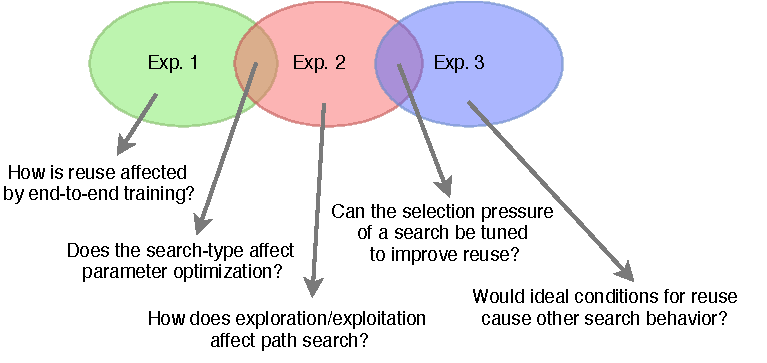
\includegraphics[width=\textwidth]{Chapters/1.Introduction/figures/All_experiments.pdf}
    \caption[Thesis questions]{Visualization of how the questions raised in this thesis is separated across the three experiments.}
    \label{fig:research_questions}
\end{figure}

Chapter \ref{exp1} investigate the possibility of arbitrarily selecting the first set of parameters for end-to-end training, instead of performing a time-consuming search through randomly initialized weights. This might save time in future experiments as there is no knowledge to reuse when the first task is learning. However, the end-to-end training might affect the optimization of the selected weights and increase the difficulty of reusing them in future tasks. A more general statement of this goal is to test if different search types and parameter training contexts affect parameter \textit{reuse}. If the results from this experiment indicate that there is no difference in parameter reuse between the two training schemes for the first task, subsequent experiments will be performed using this arbitrarily selecting of the first parameter set. 

Experiment two in chapter \ref{exp2} share the research goal of testing if different search schemes affect learning, but under a more extensive multi-task scenario with six tasks. The experiment explores how the knowledge reuse is affected by different search types, and if a search scheme can be selected to optimize this reuse. Seven algorithms are tried, where the \textit{selection pressure}(see section \ref{background:GA}) of each algorithm is different. 

The last experiment in chapter \ref{exp3} deploy the same search algorithms used in chapter \ref{exp2} in a scenario optimal for knowledge reuse. By learning the same tasks two times, all the necessary knowledge for solving the second problem is present in the PathNet. As an ideal search algorithm should be able to find the best-suited parameters for each task, this scenario might unveil interesting differences between the algorithms. The seven algorithms are tried with four different termination limits to the search to investigate if the knowledge reuse follows other patterns at different points during the search. 


\section{Thesis Outline}
\subsubsection{Chapter 1. Introduction}
Providing an introduction to the thesis as well as the motivation behind it.
\subsubsection{Chapter 2. Theoretical Background}
Lays the theoretical foundation drawn upon in this thesis. The previous work done on the PathNet structure is mentioned her.
\subsubsection{Chapter 3. Implementation}
Information about code implementation and what data is used.
\subsubsection{Chapter 4. Experiment 1: Selection versus search}
The first experiment where module permutation is done in an empty PathNet structure. The experiment explores the possibility of not performing a full path search for the first path, but rather selecting the first modules arbitrarily.
\subsubsection{Chapter 5. Experiment 2: Selection pressure}
Exploring search algorithms used for optimal module selection. Multiple searches are performed where the selection pressure of the search algorithms are different. 
\subsubsection{Chapter 6. Experiment 3: Relearning a task}
Searching for an optimal path through a PathNet to solve a task which the structure already knows. Testing if the different algorithms have search properties which provide better or worse knowledge reuse.
\subsubsection{Chapter 7. Discussion and conclusion}
Concluding the thesis is a summary of observations and conclusions drawn from the experiments.

\iffalse

\section{Motivation}
Our brains are capable of learning something based on previous knowledge without distorting that reused knowledge. This distortion, as discussed in section \ref{background:catastrophicforgetting}, is called catastrophic forgetting and is a problem addressed and to some degree solved by technologies such as EWC\cite{ewc}, PNNs\cite{progressiveneuralnetworks} and the PathNet structure\cite{pathnet}. These introduce the ability to retain parameters optimized for a previously learned task while a new task is introduced. 

However, these three solutions have limitations. EWC optimize the same set of parameters to multiple tasks, which puts restrictions on which area in parameter-space the model can occupy. PNN and PathNet both are theoretically unlimited in the number of tasks they can retain. In practice, however, restrictions on hardware and feasible training time governs the number of tasks and parameters in these structures. 

Optimizing the reuse of parameters between tasks can reduce the overall need for new capacity for each task. Efficiently applying old knowledge to new problems could, therefore, be a step towards creating vast multi-task learning systems. 

\section{Goal}
To investigate the possibilities of effective knowledge reuse, this thesis explores the PathNet structure. A Super Neural Network which forgoes the monolithic architecture of traditional machine learning models in favor of a modular approach to parameter optimization. The three experiments will address how the modular training affects the transferability of knowledge between tasks and in what area of the exploration/exploitation landscape a search algorithm should be focused.
\fi





\iffalse
\section{Problem/hypothesis}

where do i start?
Question DeepMind left unanswered is how different GAs influence task learning and module reuse. 
Exploration vs exploitation\ref{background:GA}

why this? broad answers first, specify later. 
We know PN works. would it work better for different algorithms?
logical next step from original paper "unit of evolution"




* What do modular PN training do with the knowledge? 
- More/less accuracy?
- More/less transferability? 
Test by learning in end-to-end first then PN search. 
Difference in performance or reuse?

* Can we make reuse easier by shifting focus of search algorithm?
- PN original: Naive search. Higher exploitation improve on module selection?

\section{How to answer?}
- Set up simple multitask scenarios and try. 
* 2 tasks where first are end to end vs PN
* List algorithms with different selection pressure and try on multiple tasks. 


    What is the use of a Nifty Gadget? 
    What is the problem? 
    How can it be solved? 
    What are the previous approaches? 
    What is your approach? 
    Why do it this way? 
    What are your results? 
    Why is this better? 
    Is this a new approach? 
    Why haven't anyone done it before? 
    or
    Why do you reiterate previous work? 
    What is your contribution to the field of Nifty Gadgets? 
    
    \section{What should this chapter contain?}
    Presentation of the problem or phenomenon to be addressed, the situation where the problem or phenomenon occurs, and references to earlier relevant research. 
    \subsection{Common errors}
    Problem is not properly specified or formulated; insufficient references to earlier work.  
    
    \section{Purpose}
    What can be gained by more knowledge about the problem or phenomenon. 
    \subsection{Common errors}
    The purpose is not mentioned, not connected to earlier research, or not in line with what the actual contents of the thesis.  
    
    \section{Problem/Hypothesis} 
    Questions that need to be answered to reach 
    the goal and/or hypothesis formulated be means of 
    underlying theories. 
    \subsection{Common errors}
    Missing problem description; deficiencies in the connections between questions; badly formulated 
    hypothesis.  
    
    \section{Method} 
    Choice of an adequate method with respect to the 
    purpose and problem/hypothesis. 
    
    \subsection{Common errors}
    An inappropriate method is used, for example due to lack of knowledge about different methods; 
    erroneous use of chosen method.  
\fi
\chapter{Theoretical Background}
Since Turing wrote about the imitation game\cite{imitationgame} and Rosenblatt about the perceptron\cite{perceptron}, learning machines have stayed in the minds of computer scientists and science fiction writers. 
Improvements in computation and algorithms have since then taken machine learning(ML) past human level performance in multiple areas such as image recognition\cite{youtubecats}\cite{deepface}, board games like chess\cite{alphazero} or go\cite{alphago}, TV game-shows like Jeopardy\cite{jeopardy} or e-sports such as DOTA2\cite{dota2}.

\section{Machine Learning}
\label{background:ML}
 
In machine learning, the fields of statistics, mathematics, and data analysis are combined and applied to automatic modeling of data. Its three main sub-fields, supervised, unsupervised and reinforcement learning covers a vast number of structures and techniques. However, this thesis will focus on the flag-ship of machine learning, the artificial neural network,  set it in a supervised learning scenario where it is applied to a classification problem.

\begin{figure}[ht] 
\centering
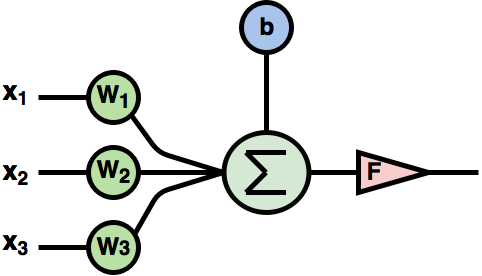
\includegraphics[width=0.7\linewidth]{Chapters/2.Background/figures/artificial_neuron.png}
\caption[Visualization of a artificial neuron]{Visualization of a artificial neuron. Each input \(x_{i}\) is multiplied with a corresponding trainable weight \(W_{i}\) before the products are all summed together with a bias \(b\). The resulting value is then passed through a activation function \(F\)}
\label{fig:artificialneuron}
\end{figure}

Supervised learning is a way to teach some machine learning system patterns in annotated data. In a dataset \(\left [X, Y \right] \), each data-point \(x_{i}\) corresponds to a label or ground truth \(y_{i}\). In the context of an Artificial Neural Network, each \(x_{i}\) is fed through the network and fitted against the target \(y_{i}\) using some optimization algorithm. 

Inspired by the structure of the brain, the \textit{Artificial Neural Network} or \textit{Neural Network} (NN) consists of layers of artificial neurons like the one visualized in figure \ref{fig:artificialneuron}. Each neuron has a number \(n\) of inputs \(x_{i}\) where each input is scaled by a tunable parameter or \textit{weight} \(w_{i}\) and summed together including a bias \(b\) before it is passed through a activation function \(F\).

\begin{equation}
    F(\sum_{i=1}^{n}W_{i}x_{i} + b) = output
\end{equation}

Two of the most commonly used activation functions are the rectified linear unit function (ReLU) and the softmax function, which is the generalization of binary logistic regression to multiple classes. ReLU merely evaluates to the maximum of neuron output and 0, which sets zero if the output is negative and keeps positive outputs. Softmax, on the other hand, approximates a probability by scaling the output of a set of neurons to have a sum between 0 and 1 and are used in classification. These two activation functions will play a role in the later experiments (see \ref{exp1:implementation} and \ref{exp2:implementation}) in this thesis, where softmax will be used as the final activation layer to be the basis of classification. ReLU is used as activation function throughout the rest of the neural networks. 

These types of systems \textit{learn} to approximate a function based on the data provided to the network. Each data point x consist of multiple features (\(x_{i}\)'s), which is fed through one or more layers of neurons that output a prediction \(\hat{y}_{i}\). This prediction is then compared to the ground truth with a loss function\footnote{Also called cost function, error function or objective function} which calculates the difference between expected output \(y_{i}\) and observed output \(\hat{y}_{i}\).
For this thesis, the loss function used is cross-entropy which is well suited for classification with softmax activation\cite{softmaxcrossentropy}.

The goal of the training is to minimize the loss function for a given data set. To accomplish this, the loss is backpropagated through the neural network, and an optimization algorithm is used to calculate the gradient of the weights with regards to the layer output and then to adjust the weights. The optimizers used in the experiments \ref{exp1} and \ref{exp2} are stochastic gradient descent(SGD)\cite{sgd} and Adaptive Moment Estimation (Adam)\cite{adam}. 

The function approximation properties of neural networks are used as a regression tool in data analysis and prediction, reward signal estimation for reinforcement learning among other areas, but is as mentioned, applied to classification in this thesis.

The final softmax layer outputs an estimated probability for each label given some input where the label given highest probability is selected as the model's prediction. As long as the input features to the network is correlated to the label in some way and there is enough training data, the neural network will adapt to the patterns in input features and learn one or more classification rules. In the case of an image classifier, the network is provided with the raw pixel values in the image. A normal, fully connected neural network\footnote{Also called affine, or dense networks.} is badly suited for this type of classification since attributes in images often change location or scale in the images \ref{exp1:implementation}. E.g., a picture of a dog is still a picture of a dog if the image is rotated upside down, rescaled, or framed differently. To account for all these cases, the dataset used would have to contain enough examples of all these variations.
\begin{figure}[ht] 
    \centering
    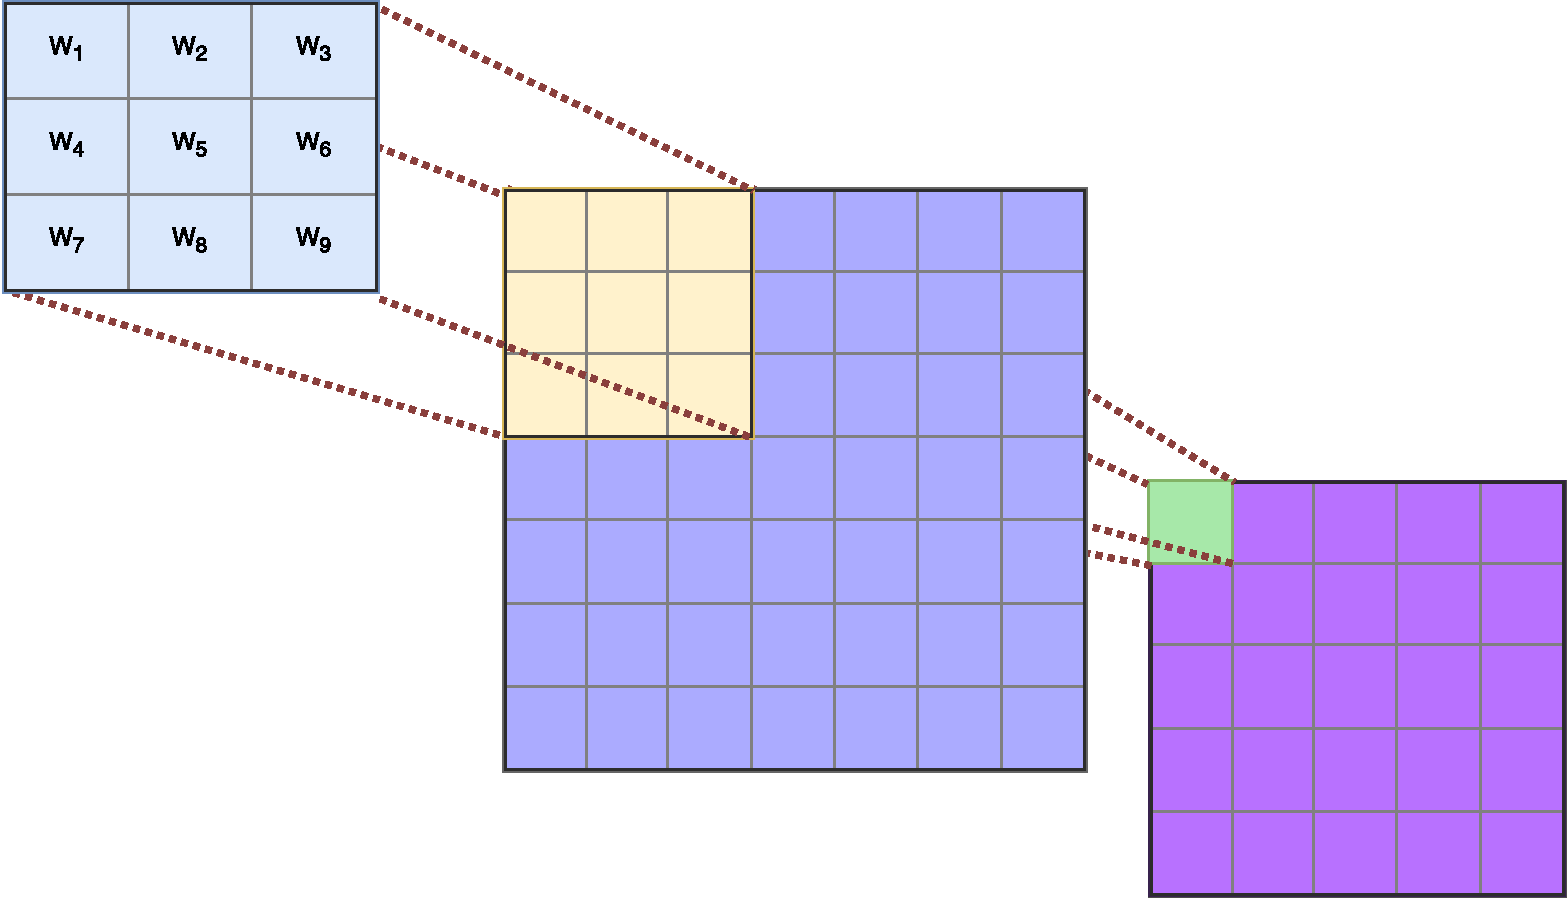
\includegraphics[width=\linewidth]{Chapters/2.Background/figures/convolution.pdf}
    \caption[Illustration of convolutional operation.]{Illustration of convolutional operation. The teal matrix contains convolutional parameters. These are element-wise multiplied by the overlapping (yellow) pixels in the image (blue) and added together. The resulting value is placed in the corresponding location in the output feature map (purple). The convolutional operation is completed by sliding or \textit{striding} the yellow window across the original image.}
    \label{fig:conv}
\end{figure}
To remedy this, image classifiers usually contains convolutional layers which are invariant to scale, rotation or translation. In a convolutional layer, a \textit{kernel} of trainable weights are convolved with the input image. This results in what is called a feature map, where the image size is reduced by some number of pixels\footnote{In some cases we would want to keep the image dimensions, in which case the input image can be padded to keep its original form.} depending on the size of the kernel. However, the depth of the image is increased, the intent is to raise the level of abstraction in the feature map for each convolutional layer. 

In a convolutional operation, a kernel is slid across an image, and for every overlap between the kernel and a image section, the kernel weights are multiplied with its corresponding pixel and summed (see \ref{fig:conv}). As with fully connected layers, the operations performed in each step is multiplication and summation, but here, each pixel in the output feature map contains some spatial information.
This spatial area covered by each feature can be controlled by the kernel size and how much the kernel is moved (called stride) between each kernel multiplication.
Networks consisting of multiple layers of convolution is called Convolutional Neural Networks (CNNs)\footnote{These are the types of modules used in implementing the quinary MNIST classification in \ref{exp1}, and the whole of \ref{exp2}}.

\begin{figure}[ht] 
    \centering
    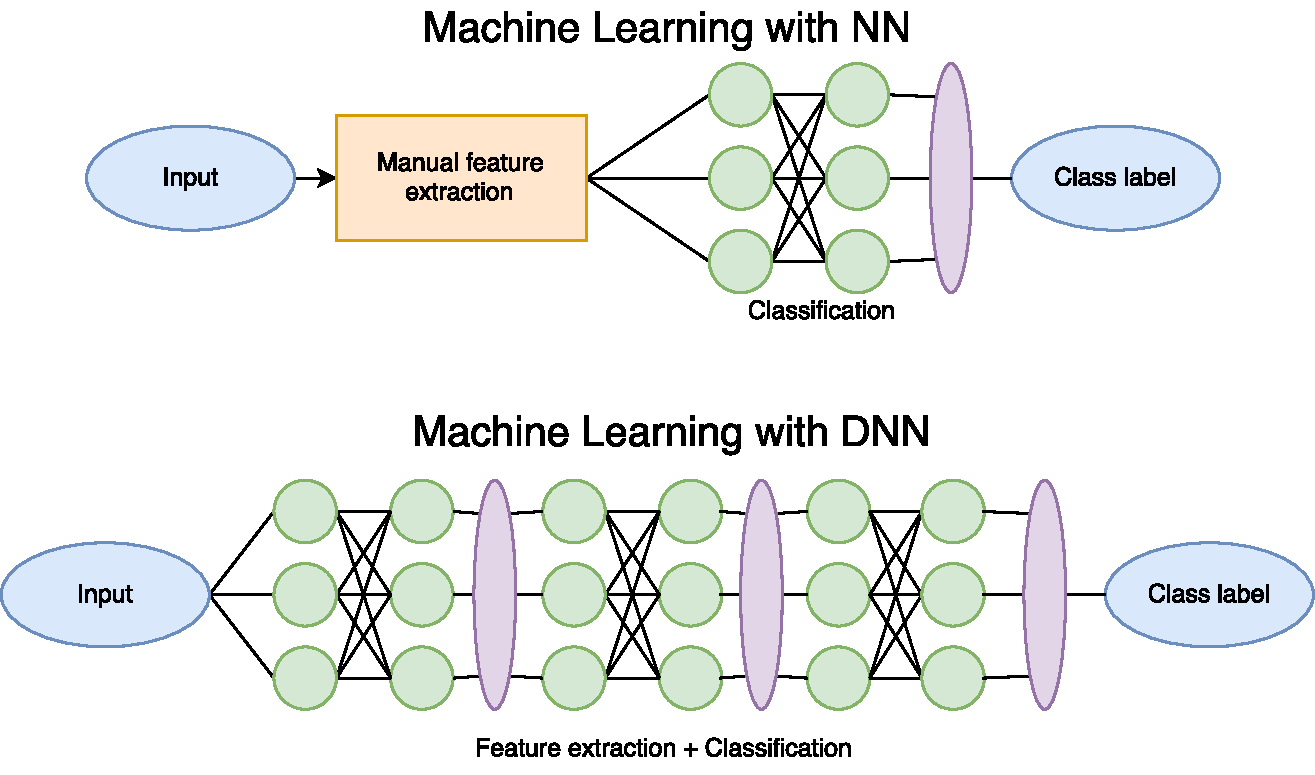
\includegraphics[width=0.8\linewidth]{Chapters/2.Background/figures/NNvsDNN.pdf}
    \caption[NN vs DNN]{Figure visualizes the difference between traditional Neural Networks and Deep Neural Networks. Artificial neurons (\textit{green}) are fully connected in both cases, and an activation layer (\textit{purple}) is set after every two layers. Where classical NN depends on being provided with high order features, the DNN performs its own feature extraction in its first layers.}
    \label{fig:NNvsDNN}
\end{figure}

\section{Deep Learning}
Usually, when talking about CNNs, the line is crossed into Deep Learning. In each layer of convolution, the spatial size is reduced while the number of channels increases. This means the information processed in step gradually shifts from a spatially encoded "image" to an encoding in feature space, making a CNN capable of turning raw image input into a higher order feature representation. That is why deep Convolutional Neural Networks can be said to be performing feature extraction on its own.

\begin{figure}
    \begin{subfigure}[h]{0.49\linewidth}
        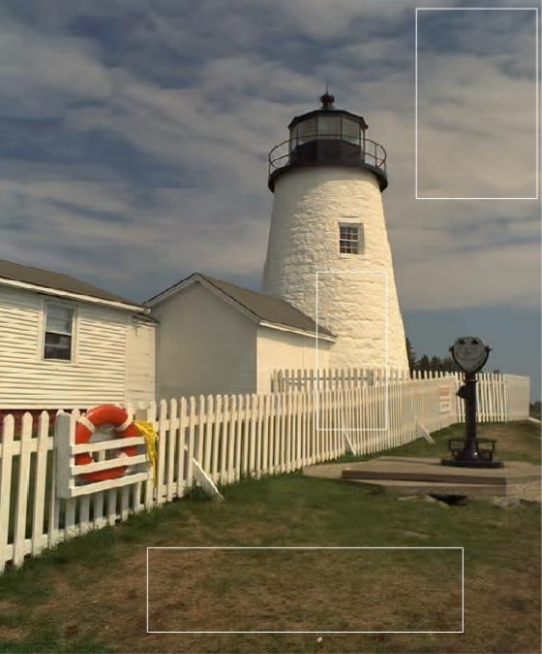
\includegraphics[width=\linewidth]{Chapters/2.Background/figures/original.png}
        \caption{Original image}
    \end{subfigure}
    \hfill
    \begin{subfigure}[h]{0.49\linewidth}
        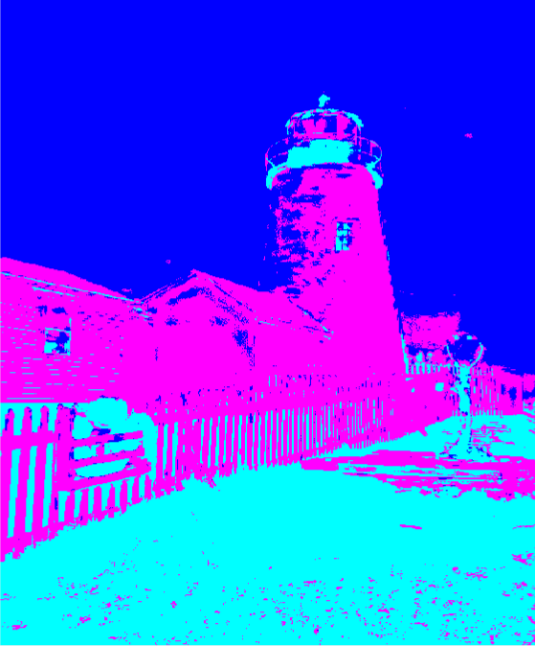
\includegraphics[width=\linewidth]{Chapters/2.Background/figures/segmentation.png}
        \caption{Segmented image}
    \end{subfigure}
    \caption[Image segmentation]{Example of image segmentation. Original image have been segmented into three classes: \textit{sky}(blue), \textit{ground}(teal) and \textit{building}(pink). The three boxes in the original image is pixels used as training data for each class.}
    \label{fig:semanticsegmentation}
\end{figure}

How \textit{deep} a DNN is made depends on the task at hand. Take for example a complicated task such as \textit{semantic segmentation}. Semantic segmentation is a variation of image classification where each pixel in an input image is assigned a class label, and the whole of the image is segmented into its parts (see figure \ref{fig:semanticsegmentation}). In a CNN performing this task, the spacial information in the original image cannot be entirely removed since we want to create a new image with the original dimensionality and spatial locations of objects. Such a neural network would need to have enough \textit{capacity} to retain all needed knowledge to complete the task. The capacity of a NN is how much information can be stored in its weights, and is a measure highly correlated to the network's number of parameters. Managing capacity needs of a NN is part of the motivation behind encouraging module reuse in experiments 1, 2 and 3 (see chapters \ref{exp1}, \ref{exp2} and \ref{exp3}).

Intuitively, the difference between NNs and Deep neural networks (DNN) is just the number of layers in the model, but functionally we can view the DNN as a collection of \textit{shallow} learning models, defined through the use of activation functions as seen in \ref{fig:NNvsDNN}. Complex Deep Learning models have been effective at such tasks as image classification\cite{imageclassification}, natural language processing\cite{deepnlp} and Reinforcement Learning\cite{deepreinforcementlearning}. The architecture and use of each of these types of DNNs are dependent on the input type and problems they are applied to as well as resource limitations.

\textbf{Edit note: Need more about DL?}

The considerable number of trainable parameters in Deep Learning increase the data resources needed. If the amount of available labeled training data is restricted, one solution is to train on a similar task for which there is a significant amount of data and apply the patterns learned to the original task. It is shown that this reuse of knowledge as a basis for further learning yields better results than what was possible with the original data set\cite{pathnet, progressiveneuralnetworks, tradaboost}. 

\subsection{Transfer Learning}
\label{background:TL}
The approach of Transfer Learning (TL) is to use generalized knowledge in one domain as a basis for future learning in another. With the goal of achieving more effective learning in the target domain or even reaching a lower convergence point for the loss, TL shares some common ground with the field of multi-task learning, where the same model is applied to multiple tasks. 

We can define transfer learning as trying to learn a target conditional probability distribution \(P(Y_{t}|X_{t})\) within a domain \(\mathcal{D}_{t}\), based on information gained from learning a source task \(\mathcal{T}_{s}\) in the source domain \(\mathcal{D}_{s}\) where \(\mathcal{D}_{s} \neq \mathcal{D}_{t}\) and \(\mathcal{T}_{s} \neq \mathcal{T}_{t}\). A domain \(\mathcal{D}\) would then, in a typical classification example, be given as \(\mathcal{D} = \{X, P(X)\}\) where \(X = x_{1},x_{2}, \dotsc ,x_{n}\) are sampled from the feature space \(\mathcal{X}\) and \(P(X)\) is a probability distribution over that space. The task \(\mathcal{T}\) in that domain would then consist of a label space \(\mathcal{Y}\) and the conditional probability distribution \(P(Y|X)\) which usually is approximated during training on a set of \(x_{i}, y_{i}\) pairs where \(x_{i} \in \mathcal{X}\) and \(y_{i} \in \mathcal{Y}\).
\newline\newline

Traditionally, transfer learning has been applied in three ways: 
\begin{enumerate}  
    \item Replacing the last layer in some trained neural network. For example, using the first layers of a CNN image classifier as feature extraction for some other image classification task 
    \item Fine tuning a trained NN by restarting a back propagation sequence for new data from a domain \(\mathcal{D}_{t}\)
    \item A combination of the prior techniques where the last layers of a network are replaced and trained from scratch, and the loss in these layers are back propagated through the rest of the already trained net.
\end{enumerate}


\begin{figure}[h] 
    \centering
    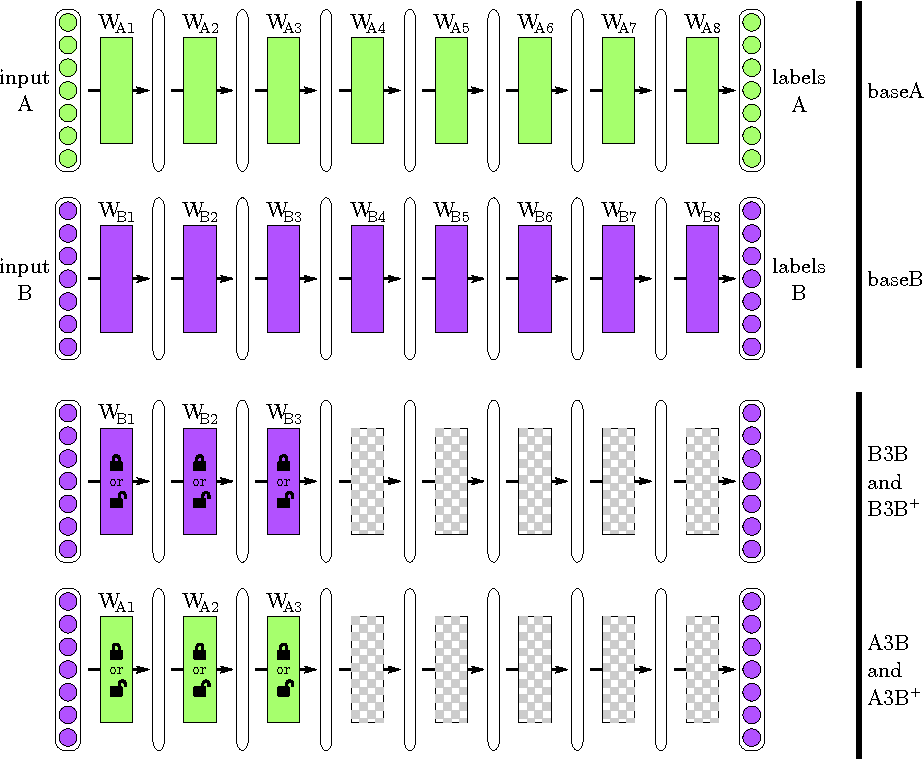
\includegraphics[width=\linewidth]{Chapters/2.Background/figures/transfer_experiment.png}
    \caption[Transfer learning experiment]{Illustration provided by Yosinski et al. in their paper\cite{yosinski2014transferable} in figure 1 to visualize their experimental process. The top two models, A (green) and B (purple), are trained first on data A then data B. The labeled rectangles represents each layer in the networks, i.e., \(W_{A_{1}}\) is the weights in layer 1 in model A, and the ellipsoids between each layer represents activation layers. The color of the stack of circles to the left of each model shows which partition of the dataset each model is trained on. The bottom two rows show the first three layers from A and B being transferred to new randomly initialized models. \cite{yosinski2014transferable} showed better accuracy in model A3B than every other model in this figure, even B3B.}
    \label{fig:transferexperiment}
\end{figure}

In a study by Yosinski et al. \cite{yosinski2014transferable}, results showed transferability in the first layers of an image classifier during an experiment proposed to measure generality and specificity in the layers as transfer performance. The study divided the data set\footnote{The study used the ImageNet dataset of 2012 which contained 1,281,167 labeled training images and 50,000 test images, each labeled with one of 1000 classes.} randomly in two subsets (A and B), and trained two identical models on each of the subsets. The first \(n\) layers in two randomly initialized models were replaced by the first trained layers from A and B. 

An additional training step, consisting of finetuning the first layers by allowing backpropagation through them, was done on data from subset B. The visualization of this in figure \ref{fig:transferexperiment} is a reconstruction of a figure in the original paper for a case with \(n=3\). The goal was to study the effects transferring had on accuracy when transferring layers from one classification case to another. 

The best results reached were achieved when training a model on subset A, transferring the first three layers to a new randomly initialized model and fine-tuning these transferred layers while using subset B to train those newly formed. This confirmed their expectation that the earlier layers in an image classifier learn to approximate Gabor-filters which are highly generalized. In section \ref{exp1:results} we see tendencies to this behavior. 

\subsection{Multi-task Learning}
Multi-task Learning and Transfer Learning both have the same ideology of sharing some parameter state between tasks to positively influence learning. Where Transfer Learning does not concern itself with performance on a seed task, multi-task learning tries to optimize parameters for multiple tasks. The most common ways of achieving this are by \textit{soft parameter sharing} and \textit{hard parameter sharing}. While both techniques have some weights unique to each task, \textit{hard parameter sharing} optimize the same parameters for all tasks. This is shown to reduce overfitting\cite{hardparametersharing} significantly. As the weights change values to optimize for a changing target, they never overly adapt to the training set. \textit{Soft parameter sharing} on the other hand have separate parameters for each task, but lateral connections between each tasks layers to minimize the distance between the parameters trained for each task.

\subsection{Curriculum Learning}
Both humans and animals learn better when examples provided are ordered and gradually increasing in difficulty. With this motivation, curriculum learning is introduced as a strategy for optimizing the learning process. This technique is shown to increase generalization to data\cite{curriculumlearning} and is the motivation for task ordering in the selection pressure experiments (see \ref{exp2:datasets}).

\section{Catastrophic Forgetting}
\label{background:catastrophicforgetting}
A problem that arises in systems where parameters are trained on multiple sequential tasks is what is called \textit{catastrophic forgetting}. Not discussed by Yosinski, but set in a transfer learning scenario, this effect manifests itself as moving parameters away from an area of low error for a previously trained task. This movement could, for instance, be because the parameters are fine-tuned for a new task. While the performance for the second task increase, performance for the first task decrease because the \textit{knowledge is forgotten} when the weights are re-adapted to the new data. This is not a problem in a scenario where the source task is considered a stepping stone to reach good performance for the target task, but might be if all tasks trained on are of the same importance.

\begin{figure}[h]
    \centering
    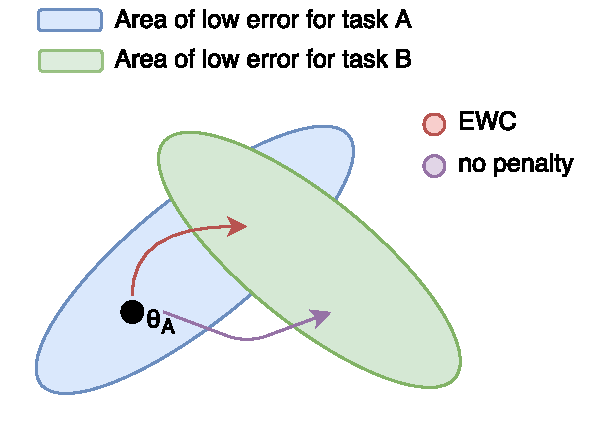
\includegraphics[width=0.7\linewidth]{Chapters/2.Background/figures/EWC.pdf}
    \caption[Elastic Weight Consolidation]{Figure from the paper on reducing catastrophic forgetting\cite{ewc}. The figure shows the parameter space \(\mathcal{P}\) and hypothetical areas of low error for two tasks A and B. The arrows indicate the direction EWC \textit{red} and normal training \textit{purple} takes the parameters.}
    \label{fig:ewc}
\end{figure}

\subsection{Elastic Weight Consolidation}
Elastic Weight Consolidation (EWC) is a novel algorithm proposed in January of 2017 by Kirkpatrick et al.\cite{ewc}. During the transfer of weights from task A to task B, over-parameterization makes it likely that a solution to problem B\footnote{A solution may be viewed as a set of parameters \(\bar{\theta}\). Neural Network training consists of adjusting these parameters through the process of backpropagation with the gradient descent algorithm. For multiple parameters in \(\bar{\theta}_{A}\), many configurations of those values will give the same performance for the NN.} lays close to the solution for task A in the parameter space \(\mathcal{P}\). During optimization of \(\bar{\theta}\) for task B, EWC makes sure the parameters stay within an area of low error for task A as seen in figure \ref{fig:ewc}

Using EWC, Kirkpatrick et al.\cite{ewc} was able to train the same NN on ten different Atari games without the effects of catastrophic forgetting between training tasks. With a human-normalized score of 1 for each game, giving a total possible score\footnote{where is 0 the same as a random agent, and 10 is at least human-level performance on all games.} of 10, the EWC driven training reached a score of around six after 500 million training frames. The control 
 never reached anything higher than 1.

\subsection{Progressive Neural Networks}
Rusu et al. published a paper in September of 2016\cite{progressiveneuralnetworks} where they addressed the problem of catastrophic forgetting during transfer learning with fine-tuning. Their proposed solution, Progressive Neural Networks (PNN) were shown to be able to learn multiple tasks sequentially without overwriting the previously trained weights. This was done by horizontally scaling the DNN with a new stack of layers for each new task.
\begin{figure}[h]
    \centering
    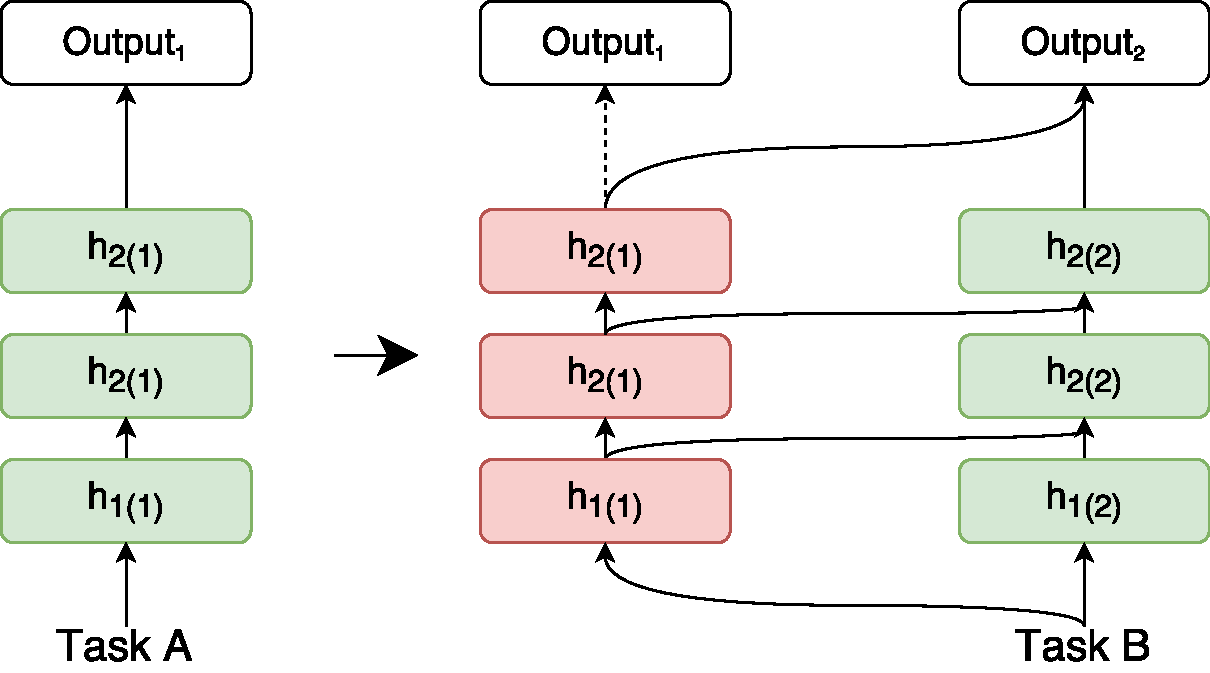
\includegraphics[width=0.8\textwidth]{Chapters/2.Background/figures/ProgressiveNeuralNet.pdf}
    \caption[Progressive Neural Network]{Example of a PNN. \textit{Left}: a three-layer NN is trained on task A. \textit{Right}: Adding another stack of three hidden layers that are being trained on task B. The weights in the first stack trained on A is now locked to the back propagation from task B, but its weights may still be used (shown by arrows between the layers). Green indicates layer is open to backpropagation, red indicates it is locked. Note that injection of a layer from an older task is not possible as lateral connections are only \textit{to} the new layer. The figure is a simplification of multiple figures from the article\cite{progressiveneuralnetworks}}
    \label{fig:pnn}
\end{figure}
After training a DNN on a task A\footnote{In the paper, the PNN was used in a Reinforcement Learning scenario.}, a new DNN was initialized with lateral connections (see fig. \ref{fig:pnn}) to the NN trained on task A and then trained on task B with back propagation only done through the newly initialized layers. This ensures that the new DNN can optimize freely on task B, but will be able to utilize the weights trained on task A, without catastrophic forgetting occurring in the first DNN. When a sufficient performance on task B is reached, the PNN can perform optimally on both tasks, given some selection of the output (i.e., if given data for a task within the domain A, the output from the weights trained on task B is not optimal). Multiple tasks can be trained using this method. For each new task, a new DNN is initialized, and the other DNNs in the PNN is connected laterally to each new layer. 

We can compare the way each new task is learned to a transfer learning scenario where backpropagation is locked in the transferred layers (see figure \ref{fig:transferexperiment}). The difference being the layer outputs are calculated in parallel for the two models, and multiple of these outputs may be introduced in the new model through what the paper calls \textit{adapters} (not visualized in \ref{fig:transferexperiment}). These \textit{adapters} performs dimensionality reduction as well as tunable scalars so the model can scale lateral connections as needed for the new task.

A problem with this scaling raised and addressed in the paper is that of quadratic growth of parameters for each new training task. Experiments show that there is a reduction in the new capacity utilized by the PNN for each new task added. This implies the growth of the PNN for each new task could decrease exponentially\footnote{Here the paper suggests pruning or online compression during learning.} without needing the new task to follow the same downward trend in complexity. 

\section{Genetic Algorithms}
\label{background:GA}
Genetic Algorithms (GA), a sub-category of evolutionary algorithms,  are biologically inspired algorithms that generate high-quality solutions to optimization and search problems. By mimicking natural operators like \textit{crossover} and \textit{mutation}, GAs views its possible solutions as individual genomes in a population and applies these natural operators on the population in a simplification of how evolution works. 

A vital driving force of GAs is the fitness-function, which maps a genome to a fitness value that can be used to rank solutions (genotypes) by how well they perform. In a real-world example of the fitness function, a \textit{strong} animal of some sort, able to acquire nourishment and fend off potential predators, is given a higher fitness value than a similar animal not as well suited for its environment. The famous term \textit{survival of the fittest} is valid in both this example and the \textit{in silico} representation of evolution. The strongest animal has a higher probability to survive and reproduce, and GAs are implemented to favor solutions that yield high fitness values.  
When a population is ranked by its fitness, different selection schemes can be applied to simulate the natural selection of strongest genomes. This selection function has a direct influence on how diverse the population is in its solutions. While we intuitively would like to remove poor solutions and keep the strong, this might guide the population only to sustain one genotype, at which point we say the population has \textit{converged}. This causes the search to get stuck in a \textit{local optima}, where the space of possible solutions have not been explored thoroughly, and we are not able to say the solution we found is among the best. Instead, the selection function varies which genomes are removed, where the more fit genotypes typically have the highest probability of survival. 

A commonly used way of ordering and discussing genetic algorithms is by the properties \textit{exploration} and \textit{exploitation}. A search with high exploration tries to keep a diverse population where many possible solution types are evaluated to find an area in solution space with high fitness. On the other hand, algorithms with high exploitation will usually find the locally best solution. A way of achieving this is by keeping a uniform population with only small differences in the genomes.

Some recombination of genomes is usually performed with a \textit{crossover} algorithm to keep the population size from shrinking each generation.  The crossover function takes a set of \textit{parent} genomes and outputs a set of offspring with the goal of controlling the population size.  Typically, a child genome is then mutated under some probability to further maintain genetic diversity. This mutation applies some small genome change.

\begin{figure}[h]
    \centering
    \begin{subfigure}[h]{0.25\linewidth}
        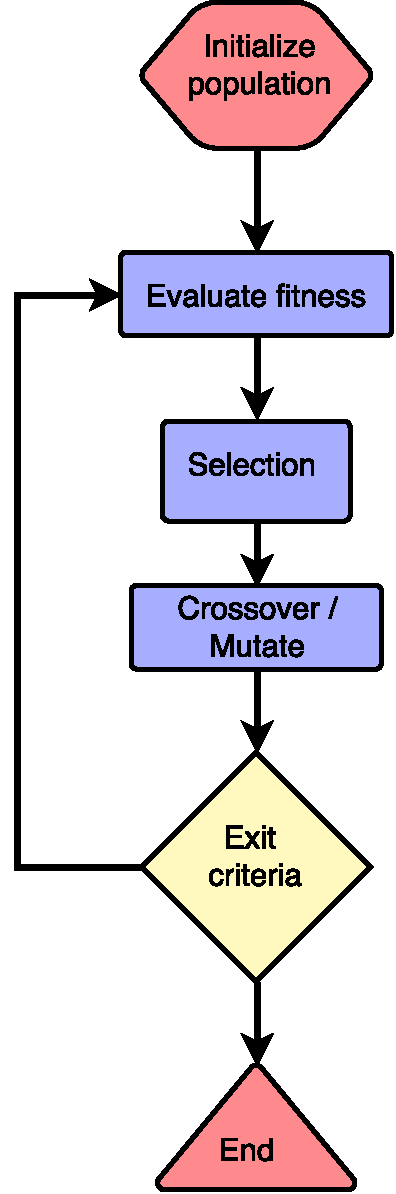
\includegraphics[width=\linewidth]{Chapters/2.Background/figures/ga_flowchart.pdf}
        %\caption{Genetic Algorithm}
    \end{subfigure}
    \hspace{0.25\textwidth}
    \begin{subfigure}[h]{0.25\linewidth}
        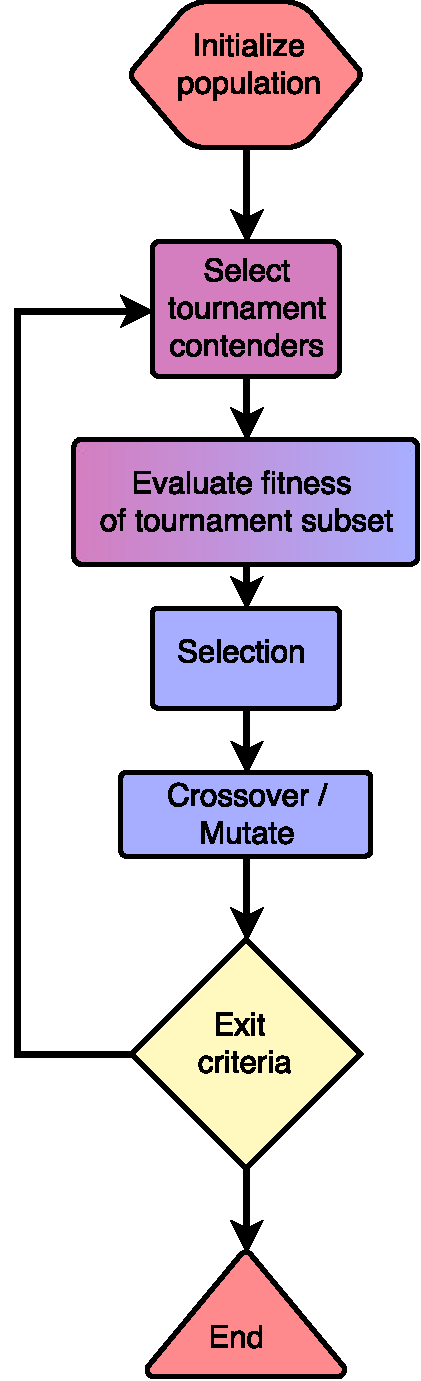
\includegraphics[width=\linewidth]{Chapters/2.Background/figures/tournamentsearch_flowchart.pdf}
        %\caption{Tournament Search}
    \end{subfigure}
    \caption[Algorithm flowcharts]{Flowcharts of the general Genetic Algorithm (left) and Tournament Search (right). The color blue indicates the operation is standard in a GA, while purple is special to a tournament search}
    \label{fig:algorithmflowcharts}
\end{figure}

\subsection{Tournament search}
One implementation of a genetic algorithm is the \textit{Tournament Search} or \textit{Tournament Selection}. True to the name, in every generation, a subset of the population is selected as contenders in a tournament. The genotypes are evaluated with a fitness function, and some selection scheme chooses genomes to be reinserted back into the population based on the fitness ranking. The selection probability is given as 
\begin{equation}
    \label{eq:tournamentsearch}
    P_{i} = p(1-p)^{i-1}
\end{equation}
where \(i\) is the fitness-ranking achieved during the tournament (1 being first place and so on) and \(p\) is the probability of selecting the first place as survivor.  

In the search implementation used in the experiments in this thesis (see \ref{exp1:implementation}, \ref{exp2:implementation}, and \ref{exp3:implementation}), a version of the tournament search is used. For every generation, a subset of the total population, given by the tournament size, is selected and evaluated. The winner then replaces each of the other contestants, making this implementation what is called a \textit{Deterministic Tournament Selection}, e.g., \(p=1\). Before the winner and its duplicate(s) are inserted back into the population, each copy of the winner is mutated under some probability to keep the diversity. 

A benefit of the tournament search, except for its efficiency in implementing and ability to work in parallel architectures, is that the \textit{selection pressure} of the search can easily be adjusted(see \ref{exp2:algorithms}). By increasing the tournament size, the winner of the tournament influence the future generations more.

\subsection{Population Diversity}
\label{background:diversity}
Population diversity is a metric assigned to a population that describes its internal difference between genomes and is mentioned here because of its importance in the experiment in chapter \ref{exp2} and \ref{exp3}. This diversity value translates to how efficiently a search explores the solution space, as the more similar the genomes in a population is, the more restricted is the search space. The goal of this metric is to provide a scalar value corresponding to the spread of genomes in genotypic space. 

Take for instance two binary genomes a and b as a population.
\begin{equation*}
    \begin{split}
        a = [0, 1, 1, 0, 0, 1, 1]\\
        b = [0, 0, 0, 1, 0, 1, 0]\\
        F_{\textit{Diversity}}(a, b)=x_{1}
    \end{split}
\end{equation*}
The diversity function \(F_{\textit{Diversity}}(a, b)\) gives a scalar diversity value \(x_{1}\). If we change the genome \(b\) to something more like \(a\), the new diversity \(x_{2}\) is smaller than \(x_{1}\) as the total diversity in the population has been reduced. 

\subsubsection{Pair-wise Hamming Distance}
One of the most commonly used measures of distance in genotypic space\cite{populationDiversity} is the pair-wise Hamming distance given by the equation 
\begin{equation}
    \label{eq:Hamming}
    H=\sum_{j=1}^{j=P-1}\sum_{{j}'=j+1}^{{j}'=P}\sum_{i=1}^{i=L}\left |y_{ij}-y_{i{j}'}\right |
\end{equation}
where P is the population size, L is the length of genome and \(y_{ji}\) is the i-th genome of genome j. In experiment in chapter \ref{exp2} a reduced form of this formula is used to calculate diversity. See appendix \ref{appendix:Hammingreduction} for reduction proof. While Hamming-distance provides a good metric for diversity, some cases can cause Hamming-distance to misrepresent a change in diversity. 

Take f.eks the populations 
\begin{equation*}
    \begin{split}
        [0, 0, 1, 1]\\
        [1, 1, 0, 0]\\
        [1, 0, 0, 1]\\
    \end{split}
\end{equation*}
which have 3 separate genotypes and a Hamming distance of 8. Reducing the diversity in this population by setting the third genome to be equal to the second changes the population to 
\begin{equation*}
    \begin{split}
        [0, 0, 1, 1]\\
        [1, 1, 0, 0]\\
        [1, 1, 0, 0]\\
    \end{split}
\end{equation*}
changes the diversity in a obvious way, but the Hamming distance is still 8 making the Hamming metric misrepresenting the diversity when duplicates of genomes appear in a population. 

\subsubsection{Frequency Diversity}
In some cases where a population contains duplicated genomes, counting the number of unique genomes can provide a more accurate diversity metric than pair-wise Hamming distance. As a diversity metric by itself, however, the frequency of unique genomes is a quite poor, as there is no nuance to the similarity. I.e., for a population of two identical genomes, changing one gene in one of the genomes would increase the diversity by the same amount as changing all genes. 

In the experiments in chapter \ref{exp2}, both frequency diversity and Hamming distance are used to create a full picture of how the diversity changes during a search.

\section{PathNet}
\label{background:pn}
In 2017, DeepMind took the modular approach\footnote{Modular with respect to the traditional approaches of transfer from monolithic models} to deep transfer learning for multi-task systems one step further with their newly developed Super Neural Network structure\footnote{A Super Neural Network is a meta-network where each node in the network is itself a Neural Network.}; \textit{PathNet}\cite{pathnet}. Where Progressive Neural Networks transfer knowledge between domains by adding a new uninitialized DNN for each task, the size of PathNet is not dynamic in the number of parameters. At training start, the net consists of randomly initialized weights in multiple DNNs, where each DNN is considered a module (or node) in a larger PathNet structure. 

Using a combination of evolutionary and machine learning techniques, PathNet shares the PNNs traits of being able to optimize for multiple training tasks without catastrophic forgetting and transfer knowledge between tasks by reusing weights locked to backpropagation.  
\begin{figure}[h]
    \centering
    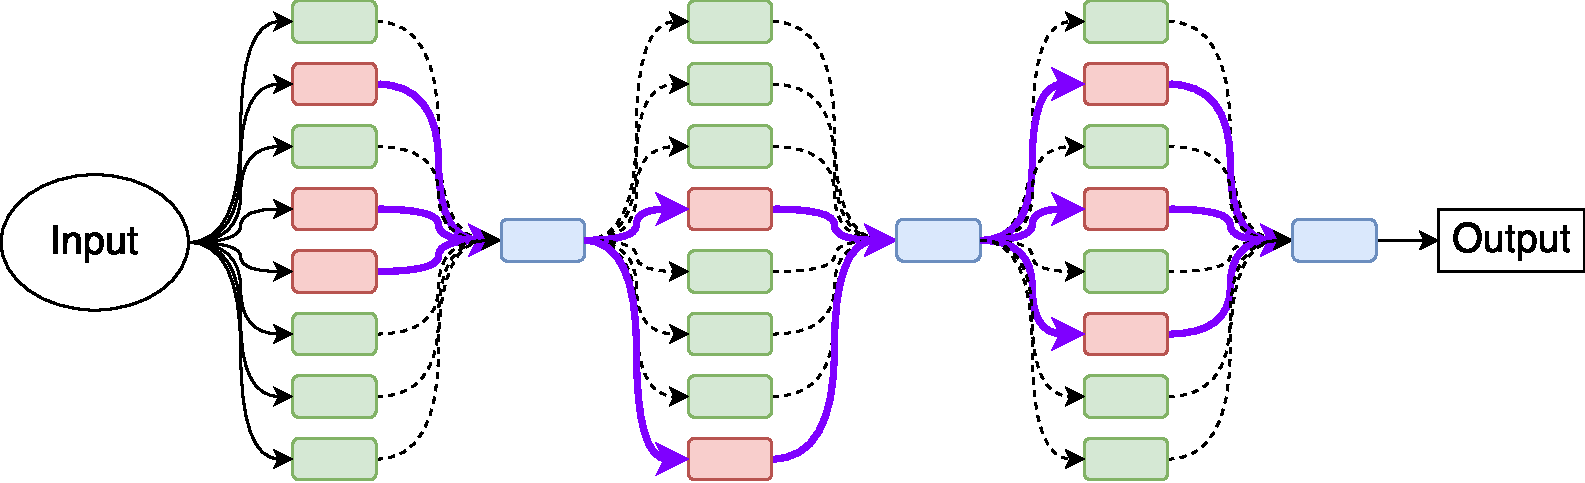
\includegraphics[width=0.8\textwidth]{Chapters/2.Background/figures/PathNet.pdf}
    \caption[PathNet structure]{Figure shows a PathNet implementation with 3 layers of 8 modules (NNs) in each layer. The \textit{red} color indicates the weights of this NN is locked to back propagation, while \textit{green} indicates it is open. \textit{Blue} cells are reduced-sum modules which summarizes the features between each layer. The purple connections show a path through the network. One path may use multiple modules from each layer, and may contain both locked and open modules.}
    \label{fig:pathnet}
\end{figure}

\subsection{Structure}
The PathNet consists of layers of modules, where each layer as a set number of modules as seen in figure \ref{fig:pathnet}. Each module is in itself a neural network of some sort, where the type of NN is adapted to the relevant task. Between each layer, the output from each active module is passed through a reduced-sum operator that adds together each output element-wise to keep the dimensionality of the output from scaling by the number of active modules. 

Each task applied to PathNet is designated a unique end-layer added to every path created for that task, meaning all paths in a search has the same final layer specific to that task. This layer defines the output and activation function that fit the problem at hand, be it a classification task, regression or something else.  

A \textit{path} is the name given a subset of the modules in a PathNet structure, where the path may contain between 1 and \(\omega\) modules from each layer, where \(\omega\) is adjusted to control the amount of capacity (number of weights) allocated to a path (solution). Each module in this path is locked after training is completed. This locking of the modules is to prevent the weights in the modules from changing if they are reused by subsequent tasks, and this preventative measure is what ensure catastrophic forgetting does not occur in this structure. After all modules in the optimal path, the rest of the modules that are not currently used and does not contain optimized weights for any task is reinitialized. Fernando et al. claims\cite{pathnet} that this re-initialization is because they were not able to reach results that outperformed fine-tuning without it.

\subsection{Search}\label{background:pathnet.search}
For every new task introduced to the PathNet, a tournament search algorithm is initialized to find an optimal path through the network. A population of pathways (e.g., subsets of modules) are randomly initialized and applied a tournament search with a tournament size of 2 and probability \(p=1\) of selecting the winner (as per equation \ref{eq:tournamentsearch}), making this tournament implementation deterministic. Every fitness evaluation of the tournament contenders is done by training them each a set amount and using the negative loss as a fitness value. One \textit{training unit} is quite small at 50 batches of 16 examples each. This means that evaluating the fitness of a path changes the performance of that path unless all modules in that path are locked to backpropagation.

When a winner is selected, the genome of the winner is duplicated to replace the looser and then mutated. Each module used in the path have the probability \(\frac{1}{L\omega}\) of being replaced with a neighboring module\footnote{A module with index \(i\) is replaced with a module of index between \(i-2\) and \(i+2\)}, where L is the number of layers, and \(\omega\) is as mentioned the max number of active modules in each layer. The rather large mutation rate ensures that the average path experience a genome change that separates it from the winner. Over multiple generations, however, the population converges to a lower diversity state where more and more paths contain similar modules. The search is terminated under some criteria, either a reached threshold fitness or a generation limit. 
\textbf{Edit note: More about pathnet needed? Implementation details? Discussion about the experiments done in \cite{pathnet}?}

\newpage

\section{Statistical methods}
\subsection{Monte-Carlo probability estimation}
\label{mc-estimate}
Given the nature of the systems used in this thesis, analytically calculating the probability of certain outcomes\footnote{In experiments \ref{exp1} and \ref{exp2}, the amount of module reuse for a random path selection is used as a comparison to experimental outcomes.} is quite hard. In such cases, the probability of certain outcomes can be estimated with a Monte-Carlo approach. This is done by simulating some scenario governed by some stochastic properties for \(n\) number of trials and measuring some \(N\) number of outcomes. The probability \(p\) of these outcomes occurring can be estimated as 
\begin{equation*}
    \hat{p}=\frac{N}{n}
\end{equation*}
Since the error here is non-biased random with a mean error of zero, the standard deviation can be given as the square root of the mean squared error 
\begin{equation*}
    \sigma=\sqrt{E[(\hat{p}-p)^{2}]} =\sqrt{\frac{p(1-p)}{n}}
\end{equation*}


Selecting a sufficiently large \(n\) can be a problem with the Monte-Carlo approach since \(p\) is unknown. Still, we can for a fixed \(n\) select a maximum standard deviation we want and calculate the size of \(p\) at which point we lose accuracy. 

For a maximum ratio between the standard deviation \(\sigma\) and \(p\) of \(R\)\footnote{I.e: \(R=0.01\) means the probability of the measured outcome is 100 times larger than the standard deviation} and \(n\) being the number of trials, we can calculate maximum of \(p\) as
\begin{equation*}
    \frac{\sqrt{E[(\hat{p}-p)^{2}]}}{p} < R
\end{equation*}
\begin{equation*}
    \frac{1}{p}\sqrt{\frac{p(1-p)}{n}} < R
\end{equation*}
\begin{equation*}
    \frac{1-p}{np} < R^{2}
\end{equation*}
\begin{equation*}
    \frac{1}{p}< nR^{2}+1
\end{equation*}
\begin{equation}
    \frac{1}{nR^{2}+1}<p
    \label{eq:montecarloP}
\end{equation}
This means if we perform a Monte-Carlo simulation of \(10^{6}\) trials and we want the standard deviation to be at most \(0.01p\) the we lose certainty if the probability is smaller than \(\frac{1}{101}\).

\subsection{Comparing results}
When comparing observations during experimentation, hypothesis-testing is a way of providing gravitas to observational differences. A method is used to test a statement about the data (called a null-hypothesis or \(H_{0}\)) by providing a p-value. This p-value is compared to a predetermined significance level (usually 0.05) and provides a metric that describes the likelihood of the null-hypothesis being valid\footnote{A low p-value corresponds to a low likelihood.}. The assumption being we can claim an assumption to be true if the counter-claim is unlikely.  

\subsubsection{Mann–Whitney–Wilcoxon test}
\label{background:mannwhitney}
When calculating a P-value, the effectiveness of the method used depends highly on the observations tested. In this thesis, we can not assume normality in the data, nor equal variance. Therefore a non-parametric method for comparison is used: Mann-Whitney-Wilcoxon (MWW) testing. This test provides a U-value used to reject or accept the null-hypothesis that two groups of observations have the same distribution. 

The assumptions laying behind the use of MWW are 
\begin{itemize}
    \item Rank-able continuous or ordinal data.
    \item Independent groups.
    \item Independencies in observations between groups.
    \item Whether the two distributions have the same or different shape is known. 
\end{itemize}
These assumptions are determined to be met in the case of these experiments. 

The cases MWW is applied here contains small groups of observations, the direct explanation of how a U-value is calculated is the quickest. 

For two groups of observations, each observation is ranked by its value\footnote{In the case of the experiments in chapter \ref{exp2} and \ref{exp3} the observations are classification validation accuracies, and each trial result is naturally ranked by this accuracy-value.}. The U-value for the group \(i\) is given as 
\begin{equation*}
    U_{i} = R_{i}-\frac{n_{i}(n_{i}+1)}{2}
\end{equation*}
where \(R_{i}\) is the sum of ranks in group \(i\) and \(n_{i}\) is the number of observations in that group. 
Calculating a \(U_{i}\) for each group tested provides two U-values where the smallest one is compared to a critical U value where the null-hypothesis is rejected if 
\begin{equation*}
    min(U_{1}, U_{2}) \leq U_{\text{Critical}}
\end{equation*}

\subsubsection{Bonferroni correction}
As the MWW rank-sum test is not multivariate, multiple tests are performed in sections \ref{exp2} and \ref{exp3} to compare all algorithms. Because the scaling probability that some of the results are unlikely, a Bonferroni correction of the significance level is done to combat the increasing probability of encountering unlikely results. 

A desired significance level \(\alpha\) is scaled by the inverse of the number of tested hypotheses \(m\). 
\begin{equation*}
    \alpha=\frac{\alpha_{\text{Desired}}}{m}
\end{equation*}




\iffalse
    x   What is the required background knowledge? 
    x   Where can I find it? 
    x   What is the relevant prior work? 
    x   Where can I find it? 
    Why should it be done differently? 
    x   Has anyone attempted your approach previously? 
    x   Where is that work reported? 
    \Section{Nifty Gadgets my way}
    What is the outline of your way? 
    Have you published it before?  
\fi
\chapter{Implementation}
\label{implementation}
Machine Learning and especially Deep Learning systems are resource intensive algorithms that need large amounts of both training data and computations. Because of the nature of computations needed for machine learning typically is large matrix operations, it is preferable to run most of the training on GPUs.

\textbf{Edit note: Need more here}

\section{Python}
Python as a programming language choice for Machine Learning is becoming more and more common. It's strength in rapid prototyping and large community that makes troubleshooting easier is heavily outweighed by the slow run time, so while Python out-of-the-box is not suited for these operations, the number of good packages for machine learning and data-processing is quite good and works around Pythons native limitations. 

\subsection{TensorFlow}
TensorFlow\cite{tensorflow} is an open source symbolic math library. It is commonly used for Machine Learning and neural network implementation as it makes it possible to design graph structures in Python. The graphs created operate on n-dimensional matrices called tensors through graphs of mathematical operations and is executed with low-level backend libraries such as \textit{C} or \textit{Fortran}.

TensorFlow also provides the support for different computing devices as needed, meaning the same implementation can be made to run on GPU with excellent benefits to computation time. The implementation used in this thesis runs all model training (weight optimization) on the GPU, but because of the substantial computation performed on the CPU between each model training, the speedup from this is not as substantial as it could be. Future implementations could take advantage of customized graph-nodes to perform tournament searches quicker. 

\subsection{Keras}
Keras\cite{keras} is a high-level Machine Learning API that has a generalized and modular approach to neural network implementation. It depends on a specialized, well-optimized low-level backend library to perform necessary tensor operations and supports the use of TensorFlow, Theano or CNTK backend. Keras provides superior debugging feedback to a stand-alone TensorFlow implementation, while it supports micro-managing of parameters through tensors or matrices.

\begin{figure}[ht]
    \centering
    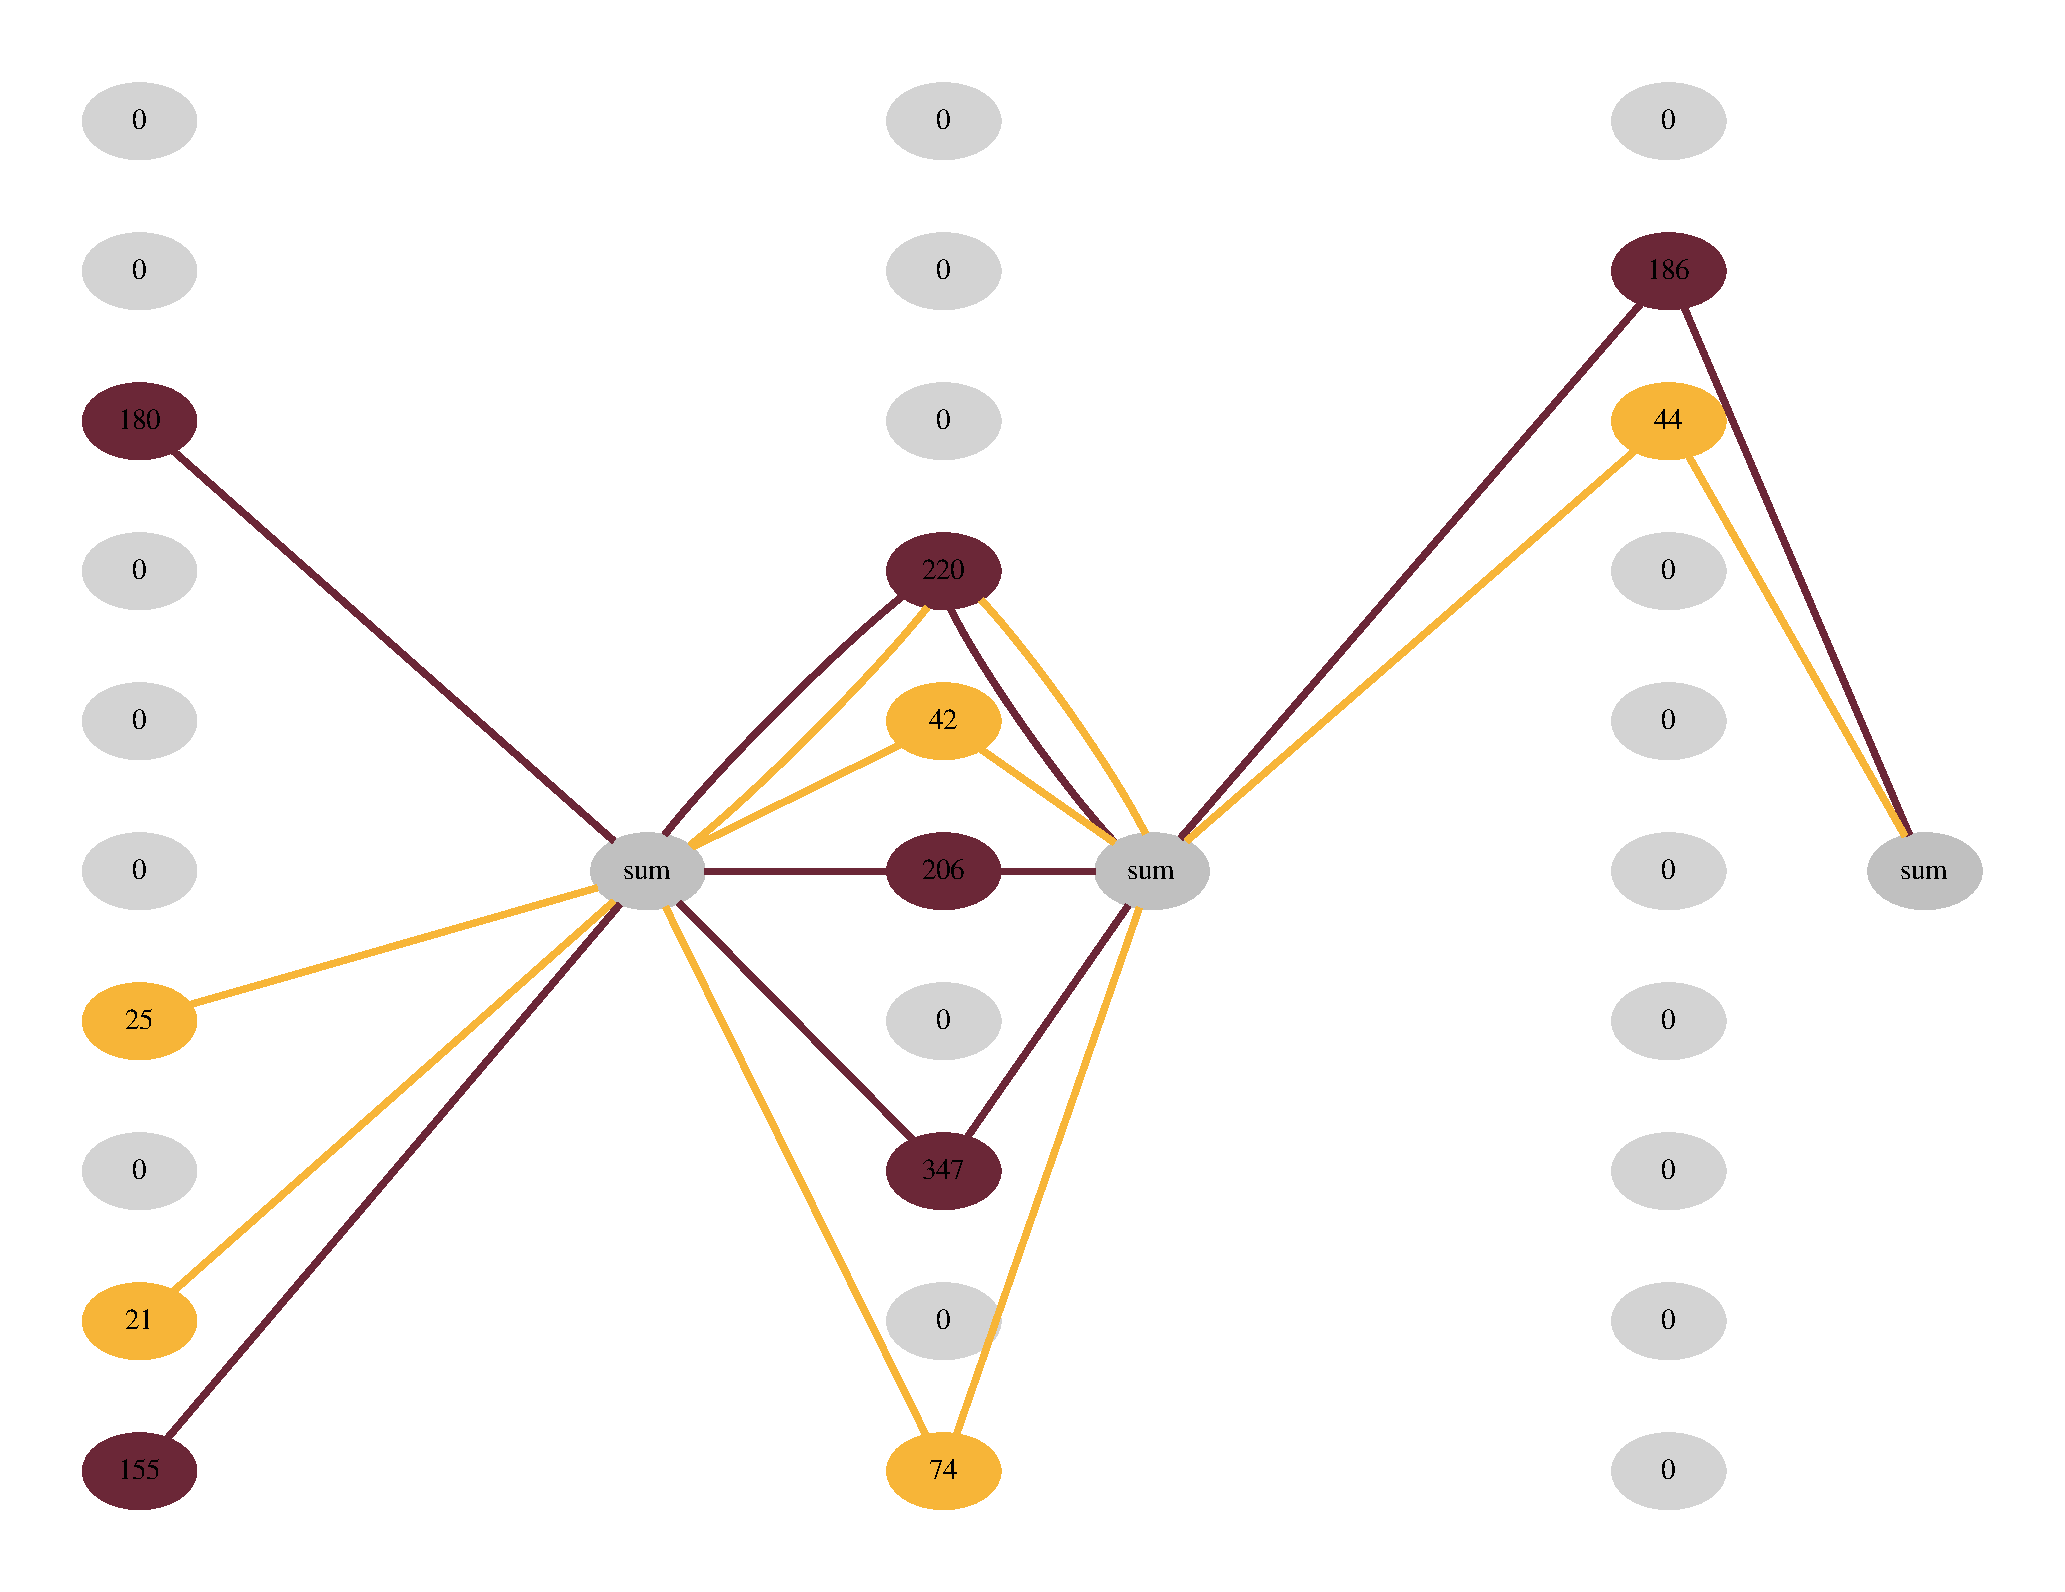
\includegraphics[width=0.8\textwidth]{Chapters/3.Implementation/figures/pathnet_visualization.pdf}
    \caption[GraphViz example]{Graph-visualization of two optimal paths through a PathNet-structure created with GraphViz. This example is of a three-layer PathNet with ten modules in each layer. The first path (red) has a total of 6 modules, and each module contains the number of training units that module have received. The second path (yellow) also use six modules but reuse one module from the first path (second layer, the fourth module from the top). Note that all modules not part of a path (gray) have undergone zero training because the weights have been reinitialized after finding the second path}
    \label{fig:pathnetexample}
\end{figure}

\subsection{Other packages}
Some other mentions to packages used during implementation of this thesis are
\begin{itemize}
    \item SciPy: Providing package containing statistical tests such as the Mann-Whitney-Wilcoxon U-test
    \item Pickle: Used during experimentation to store results and metrics.
    \item Matplotlib: Used for visualization of results.
    \item Numpy: Used for most mathematical operations not available through native Python functions 
    \item GraphViz: Used for generating graphs of PathNet structures for debugging. Multiple paths are drawn in the same graph with training amount in each module as seen in figure \ref{fig:pathnetexample}
    \item Reprint: Used to manage search terminal output by refreshing multi-line output in the terminal.
\end{itemize}

\section{PathNet implementation}
As the same code is used in multiple experiments, it is built to be easily configurable and highly modular. This object-oriented design is based around Keras's already generalized approach to Machine Learning.

\subsection{Code structure}
Modules are implemented through Layer-objects of two types: Dense layers to hold fully-connected modules and Conv layers to hold convolutional modules. Each module type is defined through a configuration-dictionary describing the NN's that constitute a module. 

\begin{lstlisting}[language=Python]
    dense = [{'out': 20, 'activation': 'relu'}, 
             {'out': 5, 'activation': 'softmax'}]
    conv  = [{'channels': 10, 'kernel': (3,3), 
              'stride': (1,1), 'activation':'relu'}]
\end{lstlisting}
In the example above, the two lists yield different module-types. \textit{dense} defines a fully connected NN with two layers, where the first layer have 20 nodes with ReLU activation and the second have a softmax activation. \textit{conv} defines a one layer CNN where the two-dimensional convolution have 10 channels, use a three-by-three kernel with a stride\footnote{As mentioned in section \ref{background:ML}, stride is how far the kernel jumps in each dimension.} of 1 in each dimension and a ReLU activation.

The Layer-objects also define other operations that can be turned on or off on instantiation through parameters. These are:
\begin{itemize}
    \item BatchNormalization in Conv-modules. This normalizes the output from a layer within each batch. The reason for this is to average potential extremes/outliers in input examples to limit radical gradients during training. \textbf{Edit note: citation}
    \item MaxPooling used after last Conv-layer. This operation reduces the dimensionality of a layer output by reducing each x-by-y\footnote{Here, only MaxPooling of 2-by-2 windows are performed. This means a 10-by-10 feature map would be reduced to 5-by-5.} window of pixels to the max value within that window. \textbf{Edit note: citation}.
    \item Flatten before the first Dense-layer. This \textit{"housekeeping"} functionality takes some n-dimensional tensor input and flattens it to a vector to be input into a fully connected NN.  
\end{itemize}

As mentioned in \ref{background:pn}, each task has its unique task-specific final layer that defines the output from PathNet for that task. This concluding layer is defined by task-objects containing one layer of fully connected nodes, an activation function, and output size specific to each task. Only classification is done in this thesis, so all tasks use a softmax activation. These object also contain some meta-info about the model they are a part of, such as input-dimensions, optimizer used for this task, a learning rate, and loss-function. 

The PathNet-object is the only one utilizing the Layer and Task-objects. Through hard-coded static methods, an initialized PathNet structure is created for each experimental run. These methods initialize all layers, modules, and configurations needed to start training. The PathNet-object also contains functionality for generating random paths and Keras-models from a given path-description and task object. It also includes a training counter for each module and an interface for updating this value. There is also some \textit{housekeeping} functionality such as saving and locking modules and a TensorFlow-session backend reset (see section \ref{implementation:problems}).

\section{Search implementation}
\label{implementation.search}
As with PathNet the search has a modular implementation for easy adaptability and reuse in all experiments. Based on a hyper-parameter dictionary, the search method uses predetermined functions for different GA operations such as selection-schemes for winner selection or path mutation. The selection-schemes used is winner-replace-all where a mutation of the winner replace all other genomes in the tournament, and a 3-to-2 scheme where the two winners of a tournament size of 3 are recombined and the offspring replace the tournament looser.

Every generation updates a Reprint-structure that gives terminal output of the search progress (see figure \ref{fig:searchoutput} for screen capture of a experimental run).
\begin{figure}[ht]
    \centering
    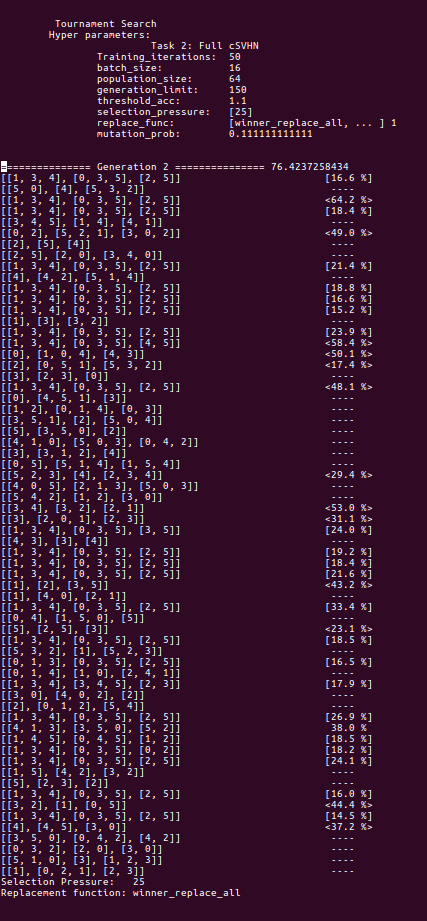
\includegraphics[width=0.6\textwidth]{Chapters/3.Implementation/figures/search_output.png}
    \caption[Terminal search output]{Screen shot of terminal output during a search. The top section contains hyper-parameters for this search as well as current generation number. Underneath the current population-state can be seen as well as some accuracies in the right margin. For these, \big[ \big] means the accuracy is outdated by training, \big< \big> means the value within is a training accuracy, .... means the path is not evaluated yet, and a plain percentage is the actual fitness of that path. At the bottom, the current generations selection pressure is printed, as well as the selection scheme.}
    \label{fig:searchoutput}
\end{figure}
\textbf{Edit note: Need more?}

\section{Notable implementation differences}
\begin{itemize}
    \item Implementation is built upon the Keras API and is more modular in its object-oriented structure
    \item Path fitness is not the negative error, but classification accuracy. 
    \item For the variable selection pressure experiment, the fitness calculation is performed after a separate training step. See \ref{exp2:implementation} for details and reasoning.
\end{itemize}

\section{Implementation difficulties} 
\label{implementation:problems}
Some implementation difficulties occurred during implementation. Most of these were due to TensorFlow effect I were unaware of. Some of the most noteworthy are listed here to help with future implementation
\begin{itemize}
    \item The TensorFlow backend session is not made for creating multiple graphs, and memory leaks can happen when memory used for graphs is not freed properly. Functionality in TensorFlow makes it possible to reset a TensorFlow session, but all graph-variables has to be reinitialized afterward. 
    \item TensorFlow's default is to use all available GPU-memory. Setting the TensorFlow-sessions GPU-options "allow-growth" parameter to 4 sets memory allocation to be done as needed.
    \item Allocated memory is not freed by TensorFlow until the Python process that initialized it is ended.
\end{itemize}

\section{Data sets}
\subsection{MNIST}\label{Implementation:MNIST}
One of the most commonly used data sets for image classification is the MNIST\cite{MNIST} set of hand-drawn digits. These 28 by 28 grayscale images contain one digit from 0 through 9 each. The 60 000  labeled images are distributed about evenly across all ten classes. 

\begin{figure}[p!]
    \centering
    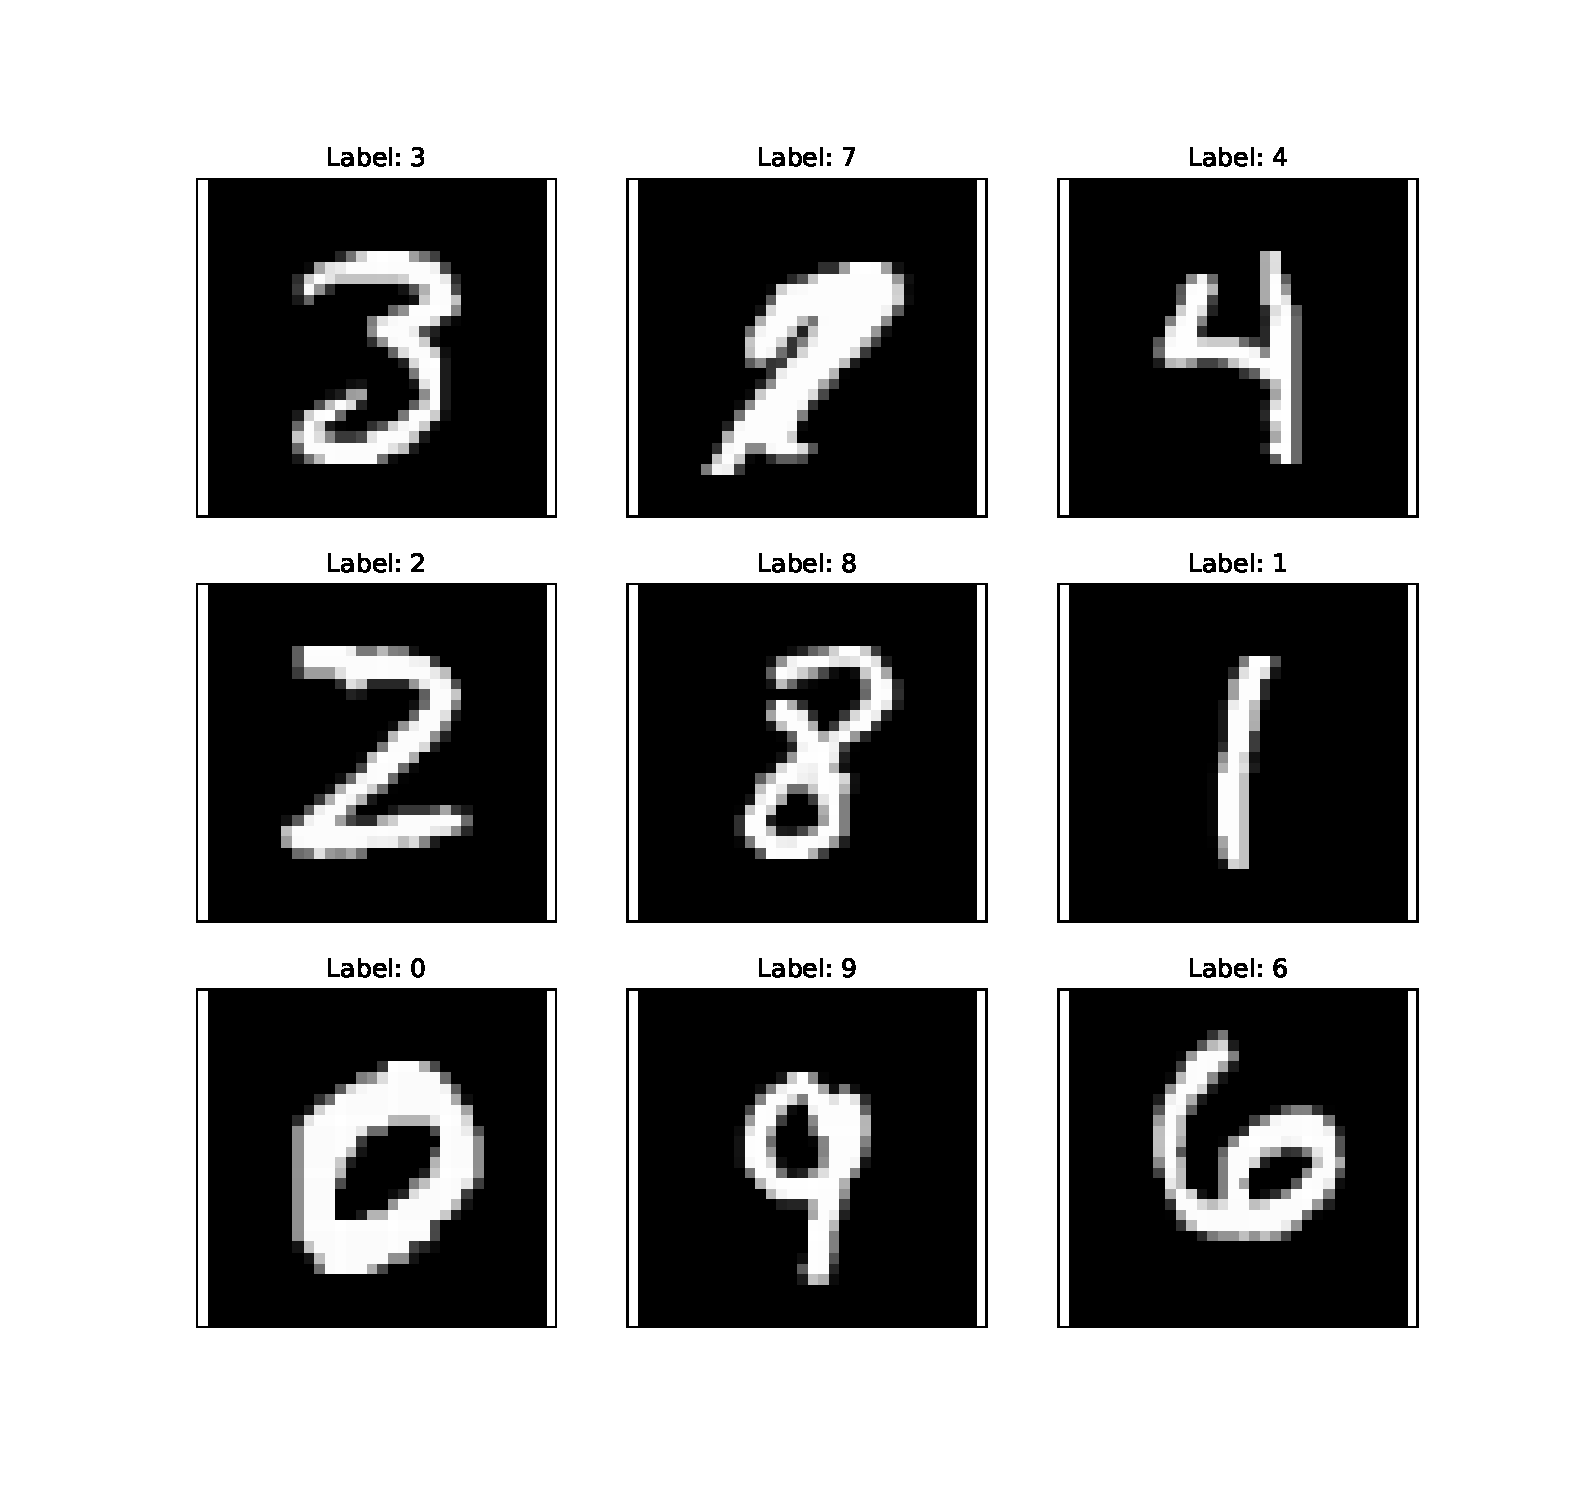
\includegraphics[width=0.8\textwidth]{Chapters/3.Implementation/figures/MNIST.pdf}
    \caption[MNIST example]{Nine images from the MNIST data set.}
    \label{fig:mnist}
\end{figure}

MNIST is a simple data set as image classification goes (see section \ref{exp1:BIN.results}). The small grayscale images contain only one small object in the middle of the image, and almost all pixels is either 0 (background) or 1 as seen in figure \ref{fig:mnist}. This makes the classification task rather easy. A list of reached accuracies\footnote{As of March 2018} can be found on the dataset's web page where it is claimed that the lowest error rate is 0.23\cite{goodmnist}, and even a KNN-classifier without preprocessing can achieve an accuracy of 97.17. 


\subsection{SVHN}\label{Implementation:SVHN}
The Street View House Number\cite{SVHN} data set is real-world images from Google Street View made for machine learning development. The original dataset contains over 600 000 variable resolution images of house numbers and bounding boxes around each digit with a label for each box. In this thesis, the version of SVHN used is made of cropped images (cSVHN) as seen in figure \ref{fig:csvhn}. These images are 32-by-32 colored images that are made to function in somewhat the same way MNIST does with a simple object and static size. Note, however, that where MNIST images contain only the object that is the basis for classification, cSVHN contain distractions (noise) in the image such as half-cropped other digits. 

\begin{figure}[p!]
    \centering
    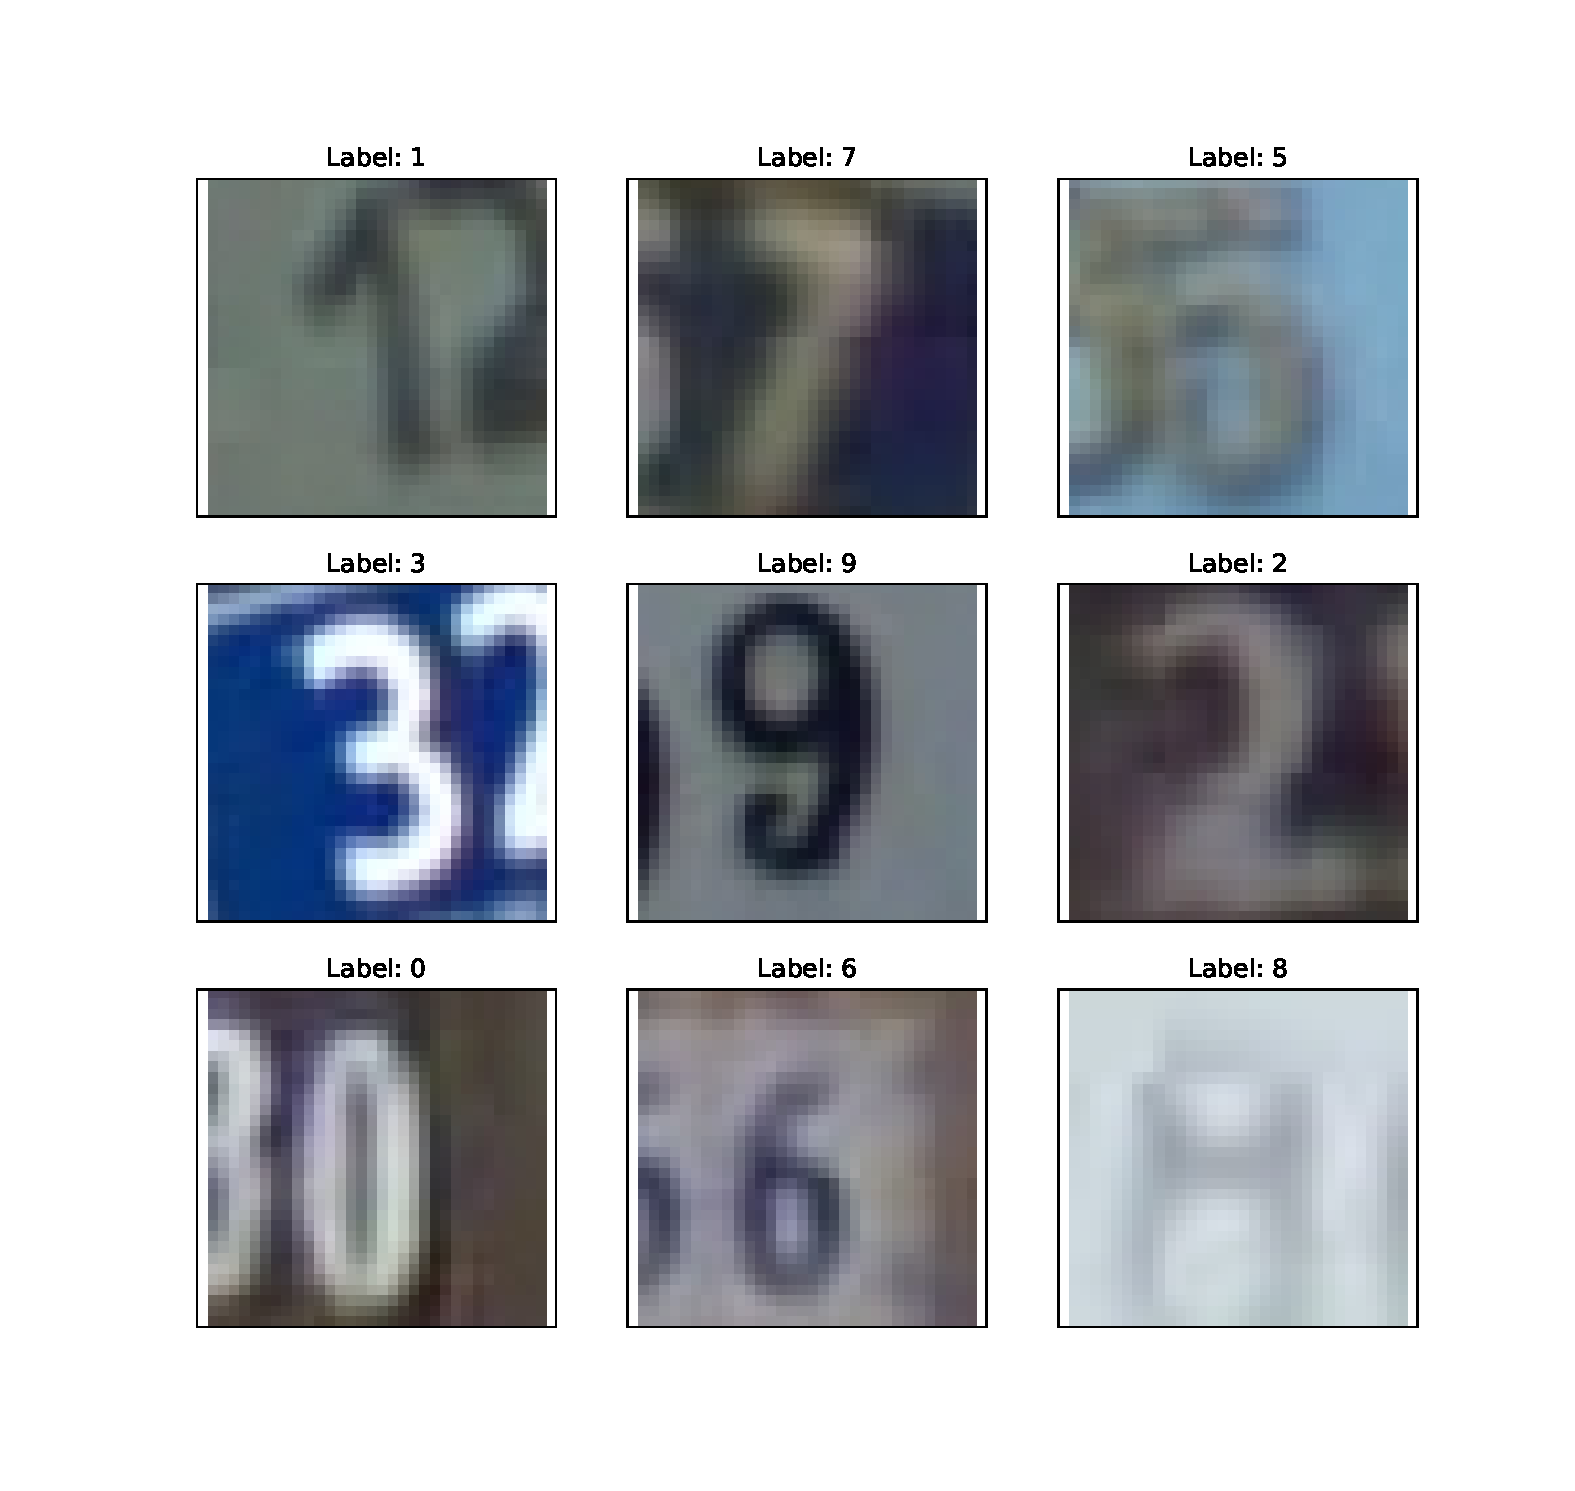
\includegraphics[width=0.8\textwidth]{Chapters/3.Implementation/figures/cSVHN.pdf}
    \caption[cSVHN example]{Nine images from the cSVHN data set.}
    \label{fig:csvhn}
\end{figure}

The whole image set is split into three sets, a training set containing 73257 digits, a test set of 26032 digits, and a simplified \textit{"extra"} image set of 531131 images, claimed by the creator to be "less difficult." This extra, simplified image set is the one used in the experiments in chapter \ref{exp2} for task 3a, 3b, and 4 and both tasks in chapter \ref{exp3}.

\begin{table}[h]
    \centering
    \begin{tabular}{ccc}
    Class number (Digit) & Number of samples & \% of whole data set\\
    0                    & 45550             & 8.6\%               \\
    1                    & 90560             & 17.0\%              \\
    2                    & 74740             & 14.1\%              \\
    3                    & 60765             & 11.5\%              \\
    4                    & 50633             & 9.5\%               \\
    5                    & 53490             & 10.1\%              \\
    6                    & 41582             & 7.8\%               \\
    7                    & 43997             & 8.3\%               \\
    8                    & 35358             & 6.7\%               \\
    9                    & 34456             & 6.5\%              
    \end{tabular}
    \caption{Distribution of samples on each class in the cropped SVHN set used in this thesis, along with the portion of the whole set each class constitute. Given a random selection of samples from this set, this percentage should approximately be the probability of selection each class}
    \label{tab:SVHN}
\end{table} 

Because these images are from the real world, and because of the nature of house numbers, the class distribution is not even. In table \ref{tab:SVHN} the number of digits in each class in the extra set is listed along with the portion of the whole set this constitutes.  

\iffalse
    X   Can you describe your implementation in detail? 
    X   Why did you use this technology? 
    X   How does the theory relate to your implementation? 
    X   What are your underlying assumptions? 
    X   What did you neglect and what simplifications have you made? 
    X   What tools and methods did you use? 
    X   Why use these tools and methods? 
\fi
\chapter{Experiment 1: Selection versus search}
\label{exp1}

\begin{figure}[th]
    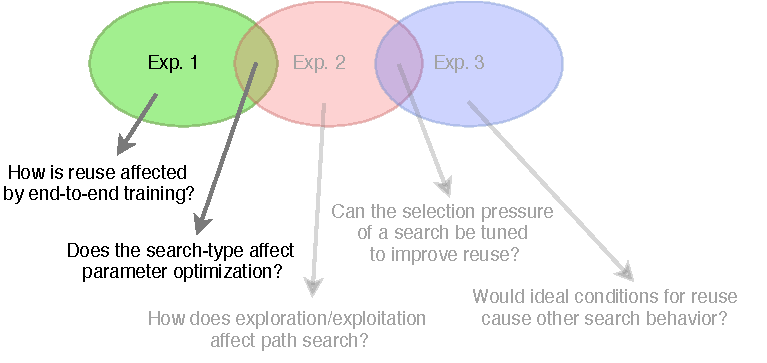
\includegraphics[width=\textwidth]{Chapters/4.Experiments/exp1/figures/exp1.pdf}
    \caption[Experiment focus]{Visualization of how the questions in this chapter fit in the larger context of this thesis.}
    \label{fig:exp1.questions}
\end{figure}
\noindent
Disregarding what algorithm is used during path searching, training multiple machine learning models are usually rather resource intensive. In the case of finding an optimal path through a PathNet, even more so. Any small reduction in the computation time here will pay dividends in future experimentation, especially when performing multiple experimental trials. Keeping this motivation in mind, the first experiment performed is one where the results either justify a shortcut in experimentation which does not introduce performance issues, or will give some insight into the development of module interfaces when applying different training schemes.

The experiments in this chapter relates to those in chapter \ref{exp2} and \ref{exp3} as seen in figure \ref{fig:exp1.questions}, and will attempt to answer:
\begin{itemize}
    \item \emph{Is there anything to gain from performing a proper search for the first path versus picking an arbitrary path and training those weights using a classic end-to-end training scheme?}
\end{itemize}


\section{Hypothesis}
It is self-evident that selecting a random path and training that subset of weights end-to-end will be more computationally efficient than a full search through a population of possible paths. A full search in a newly initialized PathNet means we are looking for modules with the most appropriate initial weights, which is a lot of labor for a rather small amount of reward. If the change of training scheme from full search to end-to-end training is shown not to affect module reuse, subsequent experiments will be performed with end-to-end training of the first task, as this will reduce search time. End-to-end training is suspected to cause the modules in the randomly chosen path to have a highly codependent interface between modules. This might then make it harder for subsequent tasks to reuse the intertwined modules, and make the encoded knowledge in those modules less transferable than in the case of a full path-search. 

When training on two tasks, the amount of module reuse between these tasks should be lower than when end-to-end training a randomly chosen path. The following experiment is proposed to test this.

\section{Description}
The experiments in this section consists of two parts. 
\begin{itemize}
    \item Search + Search (S+S): A full search for task A is performed on a newly initialized PathNet. The optimal path is saved and locked as per the PathNet design, then another full search for task B is performed.
    \item Pick + Search (P+S): A path is arbitrarily selected from the PathNet modules and trained on task A with a classic end-to-end training scheme. This path is then saved and locked normally, followed by a full search for task B.
\end{itemize}
Performing multiple runs of this experiment should show a trend in module reuse between S+S and P+S scenarios. To ensure that the first path in P+S does not have an advantage or disadvantage in total capacity,  the path found for task A in S+S is stored and used as the arbitrarily selected path for task A in the P+S scenario. This ensures that when training on task B in both the S+S and P+S scenario, the only difference is the weights along the path for task A, and the way these were reached. 

The MNIST set of handwritten digits is used for task A and B. This is because of the classification tasks simplicity and the availability of the dataset. It is also the same data used for the initial experiment performed on PathNet by Fernando et al. in \cite{pathnet}. Separating this implementation from \cite{pathnet} is that the data is kept as initially provided, and no additional salt and pepper noise is added to increase the task difficulty. 

Two experiments of this type are performed. First, a binary classification scenario. Four classes, out of the ten available in the MNIST set, is split into two groups of two classes as task A and task B. The second experiment is a quinary classification scenario where all ten classes are used in two groups of five each. The reason for the second experiment is discussed in the section \ref{exp1:BIN.discussion} of this chapter. 

\section{Hyperparameters}
\label{exp1:implementation}
The implementation of PathNet has already been described in a preceding section of this thesis, so only the hyperparameters used in the experiment will be discussed here. A list of these hyperparameters can be found in table \ref{tab:exp1.hyperparam}

\begin{table}[ht]
\centering
\begin{tabular}{lll}
                       & Binary MNIST                                                                                 & Quinary MNIST                                                                                                                                                     \\
Number of Layers       & 3                                                                                            & 3                                                                                                                                                                 \\
Number of Modules      & 10                                                                                           & 10                                                                                                                                                                \\
Module structure       & Dense only                                                                                   & Dense and Conv                                                                                                                                                    \\
Maximum active modules & 3                                                                                            & 3                                                                                                                                                                 \\
PathNet structure      & \begin{tabular}[c]{@{}l@{}}Flatten \\ Dense\\ Dense\\ Dense\\ Unique /w softmax\end{tabular} & \begin{tabular}[c]{@{}l@{}}Conv + BatchNormalization\\ Conv + BatchNormalization\\ Conv + BatchNormalization\\ Maxpool\\ Flatten\\ Unique /w softmax\end{tabular} \\
Task optimizer         & SGD                                                                                          & Adam                                                                                                                                                              \\
Learning rate          & 0.0001                                                                                       & 0.0001                                                                                                                                                            \\
Loss function          & Binary Crossentropy                                                                          & Categorical Crossentropy                                                                                                                                          \\
\# of training images   & 24754                                                                                        & 60000                                                                                                                                          \\
\# of validation images & 4157                                                                                         & 10000    

\end{tabular}
\caption{Hyperparameters used in the first-path experiments. A Dense module here consists of 20 fully connected nodes with ReLU activation, while a convolutional module is 1 channel of a 3-by-3 kernel with 1-by-1 stride and ReLU activation.}
\label{tab:exp1.hyperparam}
\end{table}

\section{Binary MNIST classification}

\subsection{Experimental setup}
A similar PathNet structure to the MNIST experiment in the original PathNet paper is used here: Three layers with a maximum of three active modules from a total of 10, each with ten fully connected nodes followed by ReLU-activation. Since each data point in MNIST is a 28-by-28 greyscale picture, the matrix of input-values is first flattened to a 784-element vector before it is used in training. The classification of digits 3 and 4 were used as task A, and digits 1 and 2 as task B. 

During the search, a population of 64 paths was used, and the search terminated when a training accuracy of 98\% was reached, or after 500 generations. During tests, searches that exceeded 500 generations usually persisted for more than 1000 generations because the parameters were stuck in a local minima. The population always converged to one path way before that point, and excessive training on a converged path would after a while approximate end-to-end training. Because of this and limitations to available experimentation time, the limit of 500 generations was enforced. For both tasks in this experiment, the task-specific classification layer that follows the PathNet's modules consists of two fully connected nodes with Softmax-activation. A total of 600 experimental trials were conducted.  

\subsection{Results}
\label{exp1:BIN.results}
\begin{figure}[t]
    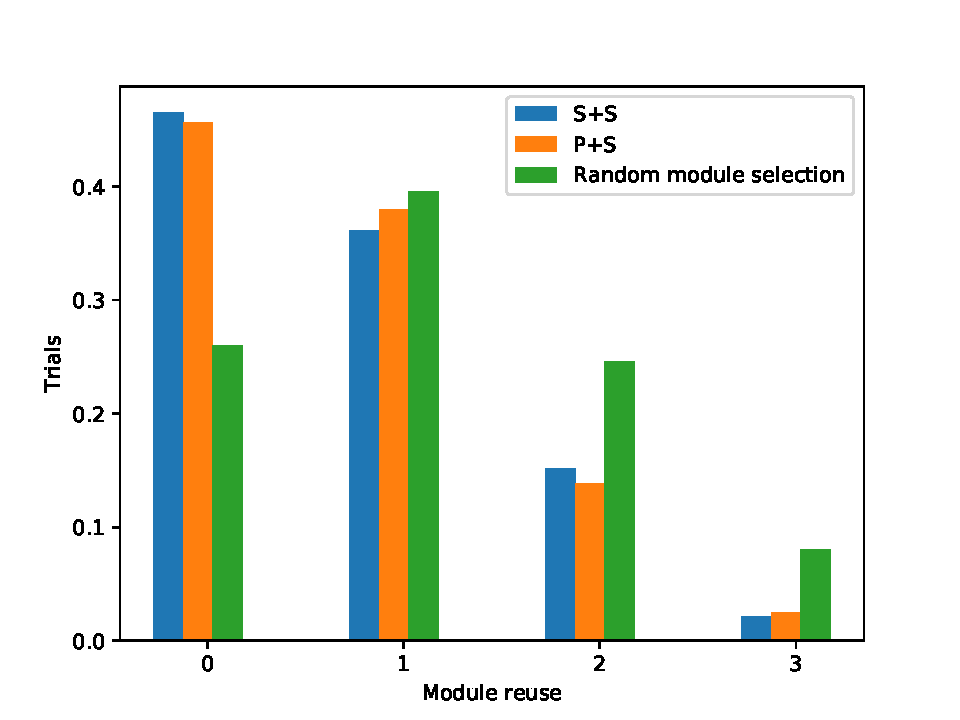
\includegraphics[width=\textwidth]{Chapters/4.Experiments/exp1/figures/BIN_module_reuse_bargraph.pdf}
    \caption[Module reuse for binary MNIST classification]{Distribution of module reuse in S+S(\textit{blue}) and P+S(\textit{orange}) searches alongside expected module reuse for randomly module selection for both tasks(\textit{green}). This plot is a result of 600 experimental runs.}
    \label{fig:binMNIST.hist}
\end{figure}

The amount of module reuse between the two tasks is visualized in three plots in terms of frequency, training, and layer-distribution.

Figure \ref{fig:binMNIST.hist} shows a bar graph of how the amount of trial is distributed on the different amounts of reuse achieved. Compared to the S+S and P+S training schemes, the expected distribution of trials for random module selection is plotted in green. No difference between S+S and P+S for any of the reuse amount is observed here. However, the amount of trials where zero reuse were found is significantly higher than expected from random module selection. Performing a Mann-Whitney rank-sum test for the two groups of module reuse show no significant difference between selecting the first path arbitrarily or searching for it with tournament search. 

\begin{figure}[t]
    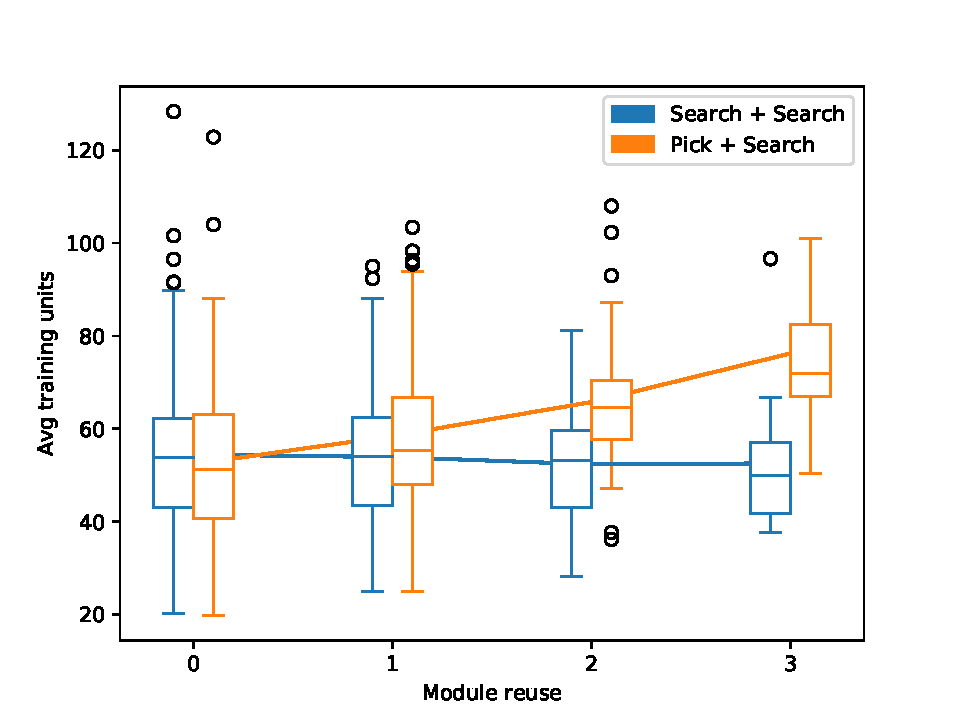
\includegraphics[width=\textwidth]{Chapters/4.Experiments/exp1/figures/BIN_training_boxplot.pdf}
    \caption[Training boxplot for binary MNIST classification]{Box-plot depicting average amount of training each module within a path gets for each group of module reuse for both P+S and S+S. Note that as the module reuse increase, the number of observations in each group decrease. Figure \ref{fig:binMNIST.hist} visualize the difference in group size.}
    \label{fig:binMNIST.box}
\end{figure}

The average amount of training units\footnote{Each module in a path undergoes one unit of training when that path is evaluated once during a search. In this case, that means 50 mini-batches of size 16.} each module in the optimal path found for task B is plotted against reuse in figure \ref{fig:binMNIST.box}. It is clear here that paths with a higher amount of reuse also have a higher amount of average training when the first path has arbitrarily been selected. The S+S scheme, on the other hand, does not seem to have any significant change in average training across the different reuse groups. 

A series of Mann-Whitney tests for each group of reuse found in figure \ref{fig:binMNIST.box} shows there is no difference in average training units for zero reuse between S+S and P+S, while the difference for 1 module reuse and higher is statistically significant under a Bonferroni corrected significance level of \(\frac{0.05}{4}=0.0125\).

\begin{figure}[t]
    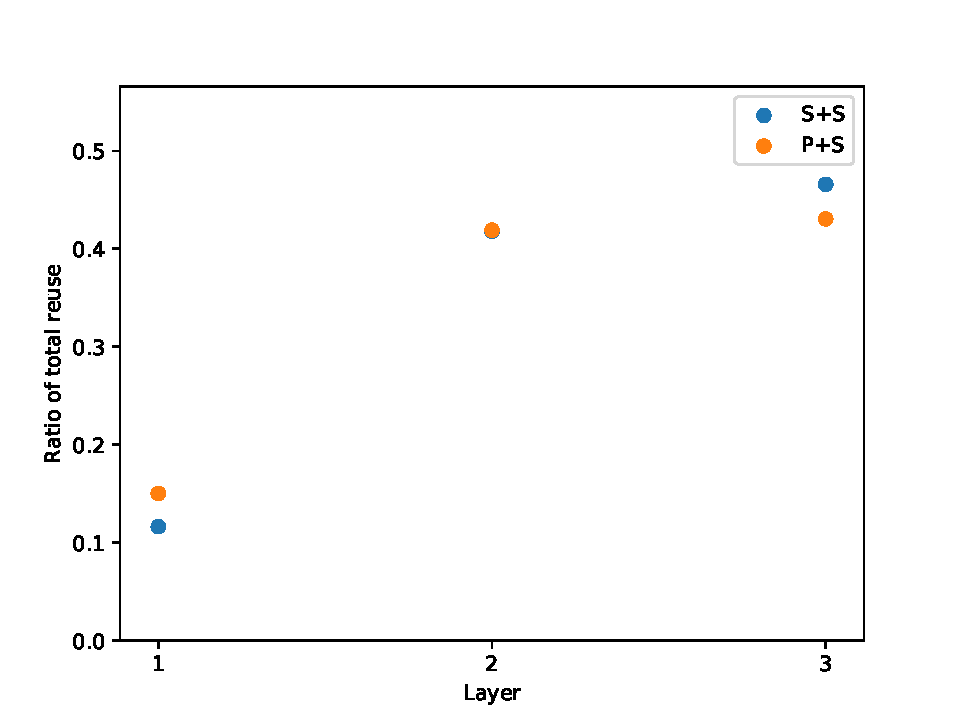
\includegraphics[width=\textwidth]{Chapters/4.Experiments/exp1/figures/BIN_reuse_by_layer.pdf}
    \caption[Reuse by layer for binary MNIST classification]{This plot shows how the total amount of reuse in all experiments are distributed on the three layers in the PathNet structure }
    \label{fig:binMNIST.layer_reuse}
\end{figure}
 
The total amount of reuse found in all experimental trials is split into which layer they occur in figure \ref{fig:binMNIST.layer_reuse}. While the difference between S+S and P+S is small, the difference between layers is quite prominent. The first layer contains significantly less of the total reuse amount at about 10-15\%. The rest of the reuse is about evenly split on the last two layers, making the distribution quite uneven. 


\subsection{Discussion}
\label{exp1:BIN.discussion}
The hypothesis stated at the beginning of this chapter would manifest itself in figure \ref{fig:binMNIST.hist} as a higher total amount of reuse for S+S than P+S. The observations do not fit under the hypothesis that end-to-end training causes confounded interfaces between layers as the two distributions seem to be equal. However, as the amount of trials with no reuse is significantly higher than expected, it might seem like the task used is too simple. This would cause the paths to train very little and the available capacity in the paths to be too high. When the distance in parameter space between initialize parameters and "good enough" parameters are too small, the gain from reusing modules cannot be justified. In other words, learning the task \textit{de novo} is simpler than learning the interface-quirks of a preceding previously used module. In that case, there would be no difference between selecting the first path arbitrarily and searching for it with a tournament search. 

As these searches are limited by a threshold accuracy, P+S might reach the same accuracy and reuse results as S+S but need more training units to get there. This is what is observed in figure \ref{fig:binMNIST.box}, where the separation between S+S and P+S is striking. Had these experiments been limited by the number of generations the tournament search is performed for, there might have been a difference in reuse in figure \ref{fig:binMNIST.hist}.

As discussed in section \ref{background:TL}, the first layer in a trained NN tend to be the most generalized as the low-level feature extraction performed by these layers are the same for most image classification. The opposite seems to be the case in these experiments, as figure \ref{fig:binMNIST.layer_reuse} would indicate. This is most likely a property of using multi-layer perceptrons as modules and would disappear if the modules in question consisted of convolutional operations. Fully connected NNs are poor at generalizing to image data because of images complex class manifolds and as a result of the raw image processing most CNN's end up performing in their first layers, convolutional layers that approximate Gabor-filters ends up being highly transferable\cite{yosinski2014transferable}.

What we see instead is that most module reuse happens in later layers in the PathNet. It is hard to tell exactly why this is, but a possible explanation is that a path contains more capacity than it needs and the later layers are capable of doing all the heavy lifting. In that case, the first layer does not contain useful weights, and therefore there is no incentive to reuse those modules. 

Since this implementation is one of fully connected nodes, each neuron has to generalize to its corresponding image pixels, and would therefore be highly task specific. This is the motivation behind performing the quinary MNIST classification experiment in addition to this one. More classes constitute a "harder" classification task, and the change from NNs to CNN's as modules should remove some of the effects we have seen in the plots in this section. Effects we expect to see in Quinary MNIST classification is

\begin{enumerate}
    \item A separation between P+S and S+S in the frequency of models with a higher module reuse.
    \item S+S should have a frequency distribution closer to the distribution by randomly choosing modules.
    \item A significantly smaller divergence between P+S and S+S in average training for each module reuse group. 
    \item An evener distribution of module reuse on each layer in a path.
\end{enumerate}

Point 4 is because the modules are changed from NNs to CNNs, and 1 through 3 because the task difficuly is increased and therefore also the necessary training time. 

\section{Quinary MNIST classification}
\subsection{Experimental setup}
A different PathNet structure is implemented here. The first two layers consist of 10 convolutional modules each, where a convolutional module contain two convolutional layers, the first with a 3-by-3 kernel and ReLU activation, and the second with a 5-by -5 kernel and ReLU activation. Following these convolutions, a Batch-Normalization layer is added to reduce the spread in gradients. The third and last PathNet-layer has 10 modules of 20 fully connected nodes and another ReLU activation. To connect the second and third layer, a two-dimensional Maxpooling reduce the dimensionality of the second layers output before the 2D matrix is flattened to a vector.   

The path searches are done with a population of 64 paths and a limitation of 500 generations, but the threshold training accuracy used here was 97.5\% to limit runtime. Since the classification tasks here are quinary, and all 10 classes from the MNIST set are used, for simplicity's sake, task A consist of digits 0 through 4, and digits 5 through 9 make up task B. 

This experiment is considerably more computationally expensive to run, so it was programmed to keep running until no more time could be dedicated to this experiment. In the end, this ended up being 535 experiments. 

\subsection{Results}
\label{exp1:results.quinary}
Each of the figures in section \ref{exp1:BIN.results} have their Quinary MNIST counterpart here, but included in these plots are a version of the S+S scheme called S+S flipped\footnote{In S+S, task A consisted of classifying the classes \{0, 1, 2, 3, 4\} while task B were classes \{5, 6, 7, 8, 9\}}, where the task order has been reversed.

\begin{figure}[t]
    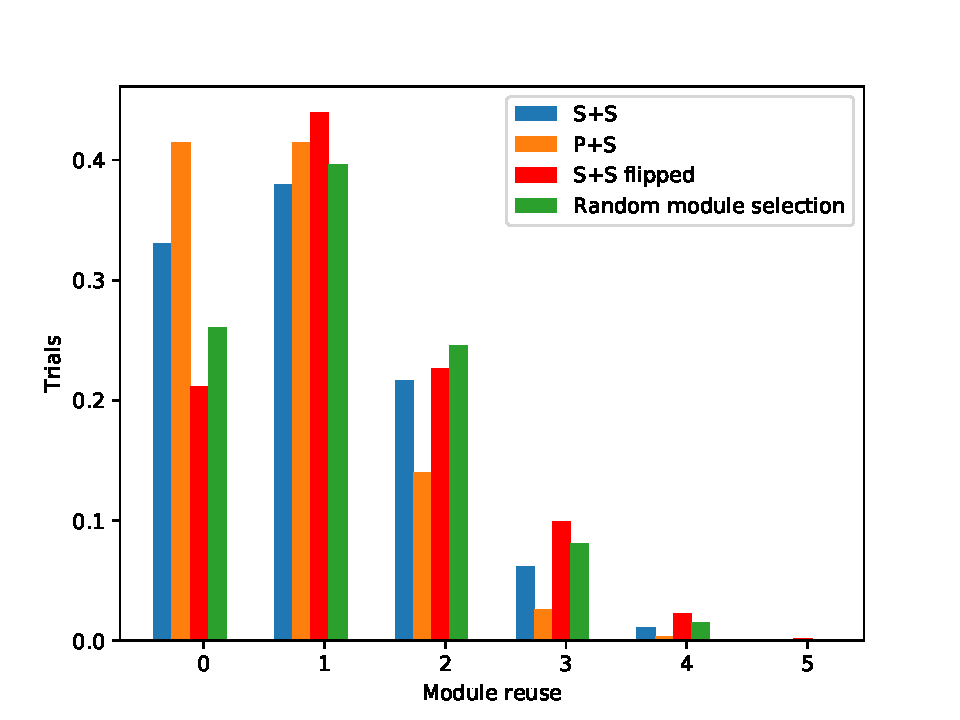
\includegraphics[width=\textwidth]{Chapters/4.Experiments/exp1/figures/QUIN_module_reuse.pdf}
    \caption[Module reuse for quinary MNIST classification]{Frequency histogram equivalent to \ref{fig:binMNIST.hist} for the Quinary MNIST classification experiment. The red bar shows reuse in a training scenario similar to S+S, but where the order of tasks is reversed.}
    \label{fig:quinMNIST.hist}
\end{figure}

\begin{figure}[t]
    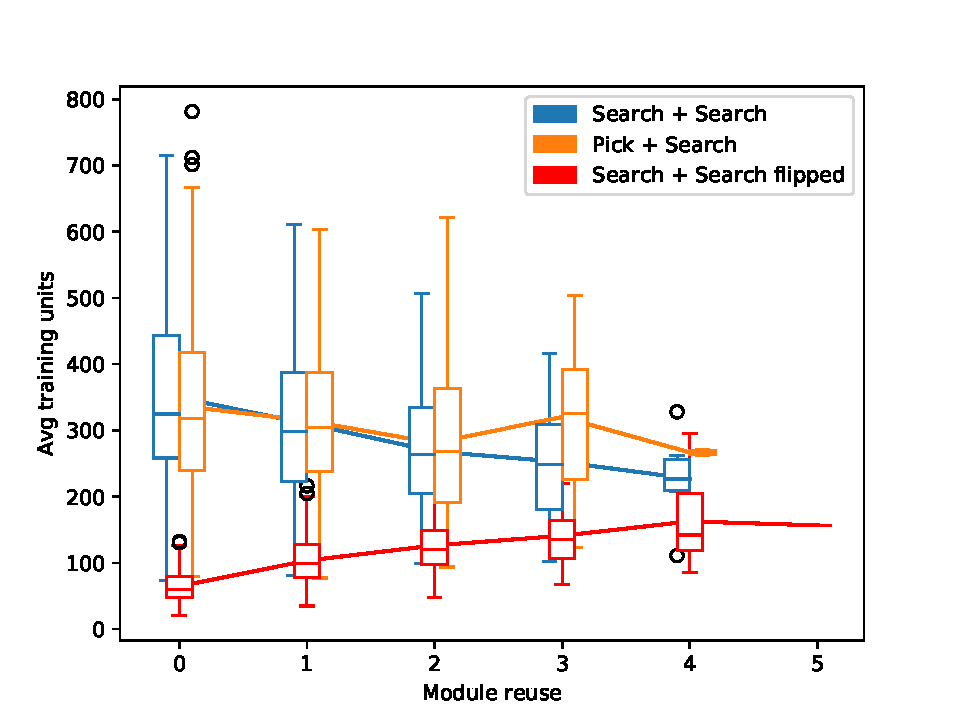
\includegraphics[width=\textwidth]{Chapters/4.Experiments/exp1/figures/QUIN_training_boxplot.pdf}
    \caption[Training boxplot for quinary MNIST classification]{Average training box-plot equivalent to \ref{fig:binMNIST.box} except for the addition of a training scenario similar to S+S but where the task order is reversed. Note that as the module reuse increase, the number of observations in each group decrease. Figure \ref{fig:quinMNIST.hist} visualize the difference in group size.}
    \label{fig:quinMNIST.box}
\end{figure}

\begin{figure}[t]
    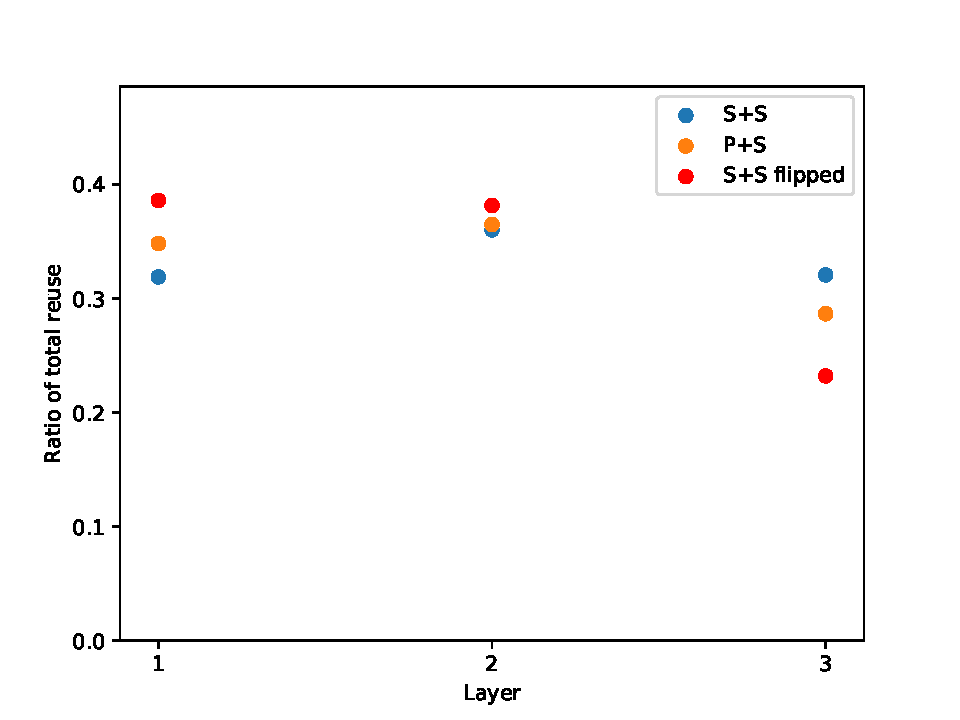
\includegraphics[width=\textwidth]{Chapters/4.Experiments/exp1/figures/QUIN_reuse_by_layer.pdf}
    \caption[Reuse by layer for quinary MNIST classification]{Frequency of module reuse for each layer in the paths. Equivalent to \ref{fig:binMNIST.layer_reuse} except for the addition of a training scenario similar to S+S but where the task order is reversed}
    \label{fig:quinMNIST.layer_reuse}
\end{figure}

It is quickly eminent from figures \ref{fig:quinMNIST.hist} and \ref{fig:quinMNIST.box} that the increase in task difficulty between binary MNIST and quinary MNIST have uncovered effects predicted in the original hypothesis. In the bar graph \ref{fig:quinMNIST.hist}, a clear difference between P+S and S+S is visible and confirmed with Mann-Whitney testing. This difference is even more prominent for S+S flipped, but as these trials have a different task order and the information contained in task B might be harder or easier to generalize, the comparison between S+S flipped and P+S is not entirely fair. 

The difference between S+S and P+S in figure \ref{fig:binMNIST.box} are not present in figure \ref{fig:quinMNIST.box}. Instead, a downward trend in average training for paths with a higher reuse has emerged. To test why this is, S+S flipped have been introduced and paths learning task B first have a trend where average training increase for a higher amount of reuse. Overall, the training for paths trained in S+S flipped is also significantly lower for all levels of reuse. Note also that the amount of training for S+S and P+S have increased from the binary MNIST classification which is to be expected due to the increase in task difficulty. 

Performing Mann-Whitney tests of S+S and P+S for the different reuse groups provides no rejected null-hypotheses proving there is no significant difference in average training between selecting and searching for the first path. Testing the difference between S+S and S+S flipped shows a significant difference for all groups but that of 4 module reuse. 

Figure \ref{fig:quinMNIST.layer_reuse} shows the uneven distribution across layers in figure \ref{fig:binMNIST.layer_reuse} is gone. For S+S flipped, the most amount of reuse is found in the two first layers.

\subsection{Discussion}
While the results in figure \ref{fig:quinMNIST.hist} does not hold conclusive evidence of the interface confounding predicted, the effect shown is strong enough to discourage the end-to-end training of a chosen first path. We saw in the results for binary MNIST classification that the number of paths with no reuse was significantly higher than expected, but this effect seems to have disappeared for S+S where it seems about the same, while S+S flipped have surpassed random module selection in reuse. Point 1 and 2 from the list of predictions seem to have been confirmed. 

Point 3 in the same list seem to have found confirmation in figure \ref{fig:quinMNIST.box}, but this plot also introduces the decrease in average training for higher levels of reuse. This effect can be explained if we suspect the task used for the first path in each experiment to be easier than the second. Say task A in a two-task system is much simpler than task B. After optimal path for task A have been found and locked, the PathNet will consist of most modules with no training, while those along path A will have a small amount. If task B is harder and more training is done during the search for path B, more reuse of modules means a higher amount of modules in path B have been trained during task A and therefore have received less training in total. The average amount of training for task B will then be lower for higher levels of reuse. 
The opposite will be true if task A is harder than task B. More reuse of modules with more training means the average training for task B will go up for higher levels of reuse. 

S+S flipped is introduced to test this, and the red boxes confirm this suspicion. While the later boxes for these results also contain a smaller amount of observation, there is undeniably an opposite trend for this task order. The over-all lower training amount might be explained the same way. If task B (classes 5, 6, 7, 8 and 9) are harder to learn, it stands to reason that it might contain more information that can be generalized to other tasks, and to generalize to that information demands a higher training effort. When S+S flipped then trains on the simple task A last, most modules in the optimal paths found did not need to undergo the same amount of training effort, meaning the average path for S+S flipped has a lower average training amount. However, the cause for this is not conclusive. 

The change from fully connected modules to convolutional modules seem to have provided results closer to what we would expect when considering results in \cite{yosinski2014transferable}. Figure \ref{fig:quinMNIST.layer_reuse} shows S+S flipped having a significantly higher reuse for the first two layers which might mean these have approximated some form of Gabor-filter. Point 4 in the quinary-MNIST predictions also see confirmation here, as S+S and P+S seem to have the same reuse distribution. 

\section{Conclusion}
In conclusion, results in quinary MNIST classification as well as the comparison with the binary MNIST experiment show promising, if not conclusive, evidence of end-to-end training causing confounded interfaces between modules and a reduction in transferability between tasks in a multi-task scenario. Note should also be taken of how task difficulty effect reuse, and ordering of task from low difficulty and upwards will manifest as lower average training for paths with a high level of reuse.

The motivation for these experiments was the possibility of reducing experimentation time by not performing a full search for the first path in the PathNet structure, but the reduction in transferability is dissuading enough not to justify forgoing a full search for all paths. 

This experiment was also prefaced by questioning the effect a path-search have on the learned parameters. Drawing upon the results in this chapter, the conclusion is that transferability of modules does depend on the context in which the modules are trained. 
\chapter{Experiment 2: Selection pressure}
\label{exp2}
In the original paper, Fernando et al.\cite{pathnet} used a binary tournament search algorithm for path optimization. The algorithm was described as "the very simplest possible agent, a unit of evolution". Binary tournament search fits this description as a "unit of evolution" because it is the minimum change that can be done on a genome level to a population.Within one generation, the total change in the population is one genotype being replaced with another from the same population and subjected to mutation under some probability. Building on the previous set of experiments where the conclusion can take form as an argument in favour of a high exploration rate during path-search, we would expect a binary tournament search to yield modules with high transferability and a high number of reuse compared to a high tournament size. In these experiments, this will be tested by manipulating the selection pressure of each search. Questions addressed in this section is: 
\begin{itemize}
    \item How would different evolutionary algorithms influence outcomes in training a PathNet structure on multiple tasks?
    \item What genetic programming strategies make the most sense in the scheme of training an SNN?
    \item How would a changing selection pressure affect learning? 
\end{itemize}
\newpage

\section{Description}
\subsection{Data-sets} 
\label{exp2:datasets}
To address these questions a trial of different searches have been applied to a PathNet structure for a selection of tasks. As with the first-path experiments, the search algorithms will be applied to image classification tasks. Building on what we learned with regards to task difficulty, two different data-sets have been selected, and the different tasks will be derived from this data. The tasks will be ordered by assumed difficulty to follow a gradual learning mentality. 

\begin{enumerate}
    \item MNIST subtasks
    \begin{enumerate}
        \item Digits 0, 1, 2, 3 and 4
        \item Digits 5, 6, 7, 8 and 9 
    \end{enumerate}
    \item Full MNIST classification
    \item cSVHN subtasks
    \begin{enumerate}
        \item Digits 0, 1, 2, 3 and 4
        \item Digits 5, 6, 7, 8 and 9 
    \end{enumerate}
    \item Full cSVHN classification
\end{enumerate}

It was shown during the first-path experiments that task 1a and 1b is not of the same difficulty level, however, within this context we will consider the training amount needed to reach a satisfactory accuracy level is similar enough for these tasks to be grouped together. The natural progression from a full MNIST classification to a SVHN is thought to increase the incentive for module reuse, even if the SVHN task will have to learn to ignore distractions in the images (see \ref{Implementation:SVHN}) that the MNIST classifiers does not have to deal with. The difference in image-dimensions have been addressed in \ref{exp2:implementation}.

As mentioned in \ref{Implementation:SVHN} there are two formats to the SVHN set, one of variable image resolutions, and one that mimic the MNIST set in static square size called cropped SVHN (cSVHN). cSVHN is selected for these experiments in order to use a constant input size to the PathNet. Within the larger set of cSVHN images, a subset described as containing "somewhat less difficult samples" is used. To increase the number of tasks, the rest of the data in SVHN could be used and noise could be added to the images to increase the task difficulty artificially. 

For both the MNIST and cSVHN set, the amount of training data have been limited to 10000 training samples and 4000 validation samples. Of these samples, MNIST have a fairly even distribution on each class while SVHN have an imbalance in the class distribution. Since the samples used are randomly selected before each experimental run, the probability of selecting one sample from a given class can be derived from the total amount of samples in that class (see \ref{Implementation:SVHN} for the exact number of samples in each class).

Each experimental run will apply a searching scheme to find an optimal path in a gradually increasing knowledge base within a PathNet. This means, for instance, tasks 1a always will be learned in a module set of only initialized weights and no previous knowledge. It is assumed that with a different ordez
\begin{enumerate}
    \item Constant selection pressure
    \begin{enumerate}
        \item Tournament size 2
        \item Tournament size 25
        \item Tournament size 3 + recombination
    \end{enumerate}
    \item Scaling selection pressure
    \begin{enumerate}
        \item Low to high pressure: 2, 5, 10, 15, 20, 25
        \item High to low pressure: 25, 20, 15, 10, 5, 2
    \end{enumerate}
    \item Dynamic selection pressure
    \begin{enumerate}
        \item Gradual change from 2 to 25 over all generations
        \item Gradual change from 25 to 2 over all generations
    \end{enumerate}
\end{enumerate}
In total, the seven tournament algorithms are used 10 times each within a reinitialized PathNet structure to train on all tasks discussed in \ref{exp2:datasets}. Between algorithms, the only hyper-parameter change is the tournament size and replacement method within each tournament. All algorithms except 1c use a winner-replace-all scheme where the mutation of the strongest paths genome replaces each of the loosing contenders in the tournament. In algorithm 1c, three contenders are selected randomly from the population and evaluated. The two strongest genomes are labeled as parents and (starting with the winner) takes turns copying their layers to the offspring. The offspring is then subject to some mutation under the same probability as every other algorithm, and replaces the loosing genome in the tournament.
\begin{figure}[ht]
    \centering
    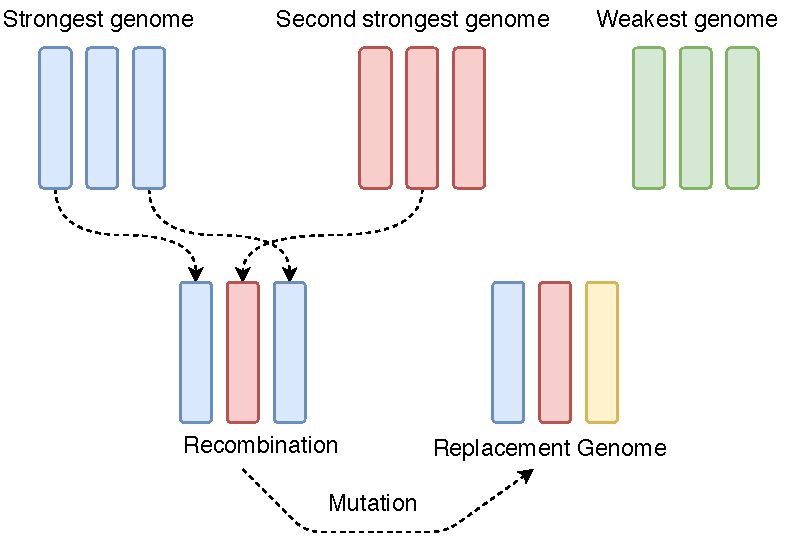
\includegraphics[width=0.8\textwidth]{Chapters/4.Experiments/exp2/figures/Recombination_algorithm.pdf}
    \caption[Recombination algorithm]{Visualization of the recombination in algorithm 1c. In a three layer PathNet, the first and last layer in the recombination would be layer one and three in the winning genome, while layer two would stem from the second strongest genome. After a mutation of the recombination, the new genome replaces the loosing contender. Each color represents one genome from the tournament and yellow represents a mutation.}
    \label{fig:search.recombination_algorithm}
\end{figure}

Algorithm group 2 consists of two algorithms where the tournament size is changed between each task. This means algorithm 2a uses tournament size 2 for task 1a, task 1b uses tournament size 5 and so on until the last task of full cSVHN classification which uses tournament size 25. In algorithm 2b, this order of tournament sizes is reversed. It is expected that in visualization of metrics where a population average is calculated for each generation, such as training accuracy, an algorithm with high selection pressure will have abrupt value changes from one generation to the next. Low selection pressure would then give a more gradual change in such values. A change between these two curve types should be prominent for algorithms 2a and 2b.

Algorithms 3a and 3b have its selection pressure changed during each tournament search. This means each algorithm behave the same for each task, which algorithms 2a and 2b did not. The change in selection pressure is gradual which means between tournament sizes 2 and 25, each tournament size is used about 4 times for a search termination limit of 100 generations. It is obvious that an even distribution of tournament sizes on each generation is not possible when using a threshold accuracy as search termination, which is one reason searches in these experiments are limited by number of generations instead. 

\subsection{Metrics}
\label{exp2:metrics}

\subsubsection{Modular reuse}
As with the first-path experiments, module reuse between tasks will be an important metric for these experiments. One unit of modular reuse is counted if a path contains a pre-trained module. In a multi-task scenario with more than two tasks, a module might be reused in more than one path and are in those cases counted once for each path reusing it. When discussing the properties of each algorithms modular reuse, it is the cumulative reuse for each task that is used.

Modular reuse is assumed to be an appropriate metric to describe the transferability of the knowledge a module acquire during training. It is also assumed that modules are able to contain some form of "memetic"\footnote{Memetic is used here to describe a quantification of knowledge in the same way "meme" is used by Richard Dawkins\cite{selfishGene} to describe a unit of cultural knowledge, here as a unit of knowledge used to solve a task.} unit knowledge

\subsubsection{Capacity use}
Highly correlated to reuse, the total amount of modules used (capacity) provides a measure of how efficiently the possible parameters are used for each task. The complexity a classifier is capable of describing is governed by the amount of available capacity in that classifier, where capacity is the amount of tunable\footnote{Here the capacity used by a path can include locked modules, which make them non-tunable.} parameters allocated to the task

\subsubsection{Validation accuracy}
When discussing classifiers, validated classification accuracy is a natural metric to discuss. However, under these circumstances, the accuracy will be affected by the training amount, which is changing across algorithms. Accuracy will, therefore, be viewed in the context of the total amount of training units applied to each path. The definition of a training unit is described in section \ref{background:pathnet.search}.

\subsubsection{Population diversity}
The change in population diversity during each search will be used to rank each algorithm by its selection pressure as it should provide a clear indication of an algorithms convergence rate. As discussed in section \ref{background:diversity}, both pair-wise Hamming distance and unique genome frequency will be used.


\section{Hypothesis}
\label{exp2:hypothesis}
The expectations for these experiments were heavily influenced by the results of the first-path experiments in chapter \ref{exp1}. When the training algorithms are viewed in a simplified context of only "exploration vs exploitation", we can place them on a scale between these extremes and discuss expected outcomes from each end of the spectrum. In this context, the Pick+Search learning scheme used in the first-path experiments would fall on the exploitation side as only one permutation of modules is tried.

In terms of tournament size, it is expected that the searches using lower tournament sizes have a lower selection pressure than algorithms using a high tournament size. This is a natural assumption to make considering the changes made to a population in each generation. Algorithms using a winner-replace-all\ref{implementation.search} replacement scheme change all genomes that is a part of the tournament except for the winner, which means the larger tournament sizes causes a larger change in the overall population. The winner of a large tournament is more favoured than the winner of a smaller tournament, making the pressure for being selected (winning) higher. 

During a search, a populations diversity shifts from an initialized state of high diversity towards a lower diversity where some optimal path can be found. As discussed, a large tournament size causes rapid changes in a population compared to a low tournament size, where the diversity drops from one generation to the next when the winning genome is duplicated. This rate at which a population converges toward a low diversity is therefore expected to be highly correlated to the tournament size.

A population is said to have converged when the diversity can not feasibly be reduced further due to mutation. Each tournament after that point would only consist of small mutations of the same genotype, making the search performing something on the order of end-to-end training as seen in the previous experiment. 

\begin{figure}[ht]
    \centering
    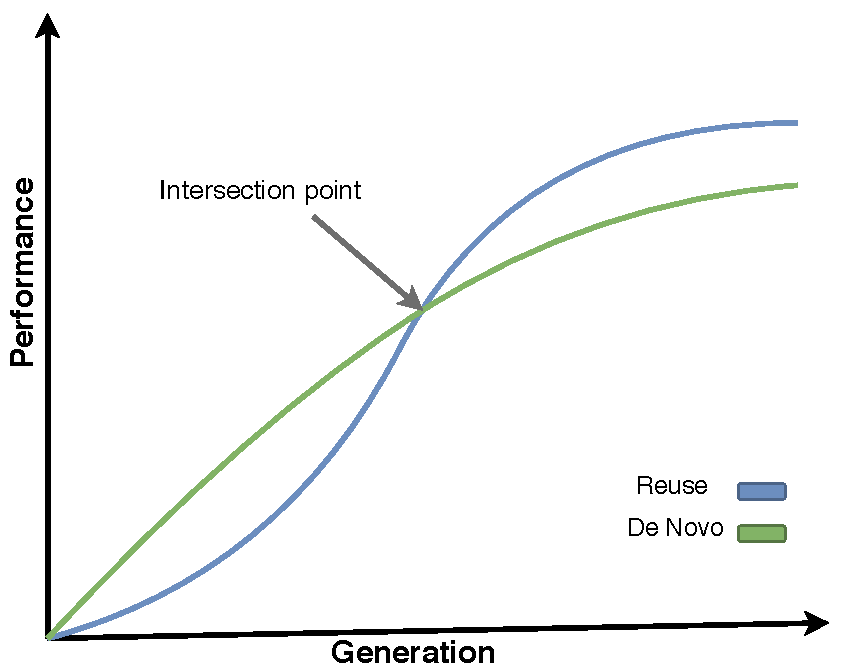
\includegraphics[width=0.8\textwidth]{Chapters/4.Experiments/exp2/figures/reuse_vs_new.pdf}
    \caption[Hypothetical performance plot]{A hypothetical plot of performance changing during a search. The two curves represent the performance of two paths where one have a lot of reuse(blue) and the other train all modules \textit{de novo}(green). The point at which reuse becomes advantageous is marked as "intersection point".}
    \label{fig:reuse_vs_new}
\end{figure}

In chapter \ref{exp1}, task difficulty was used to explain why searches resulted in using less pre-trained modules than if modules were selected randomly. We can use this effect as a definition of a task being too simple. For a scenario training on a such a task, performance of a path consisting of modules being trained \textit{de novo} would improve quicker than the performance of a path with a lot of reuse. A hypothetical scenario is plotted in figure \ref{fig:reuse_vs_new} where it is easier to train new module than learning the interface of locked modules. If the selection pressure of an algorithm is low enough for the population to converge before the intersection point between the two performance curves, training new modules from scratch would be seen a heavily favoured by the algorithm.  Algorithms that converge after that point would have a higher likelihood of reusing modules as they have enough "search time" to learn the locked module interfaces. A high selection pressure algorithm with a rapid convergence will have a higher likelihood of converging before the intersection point and we would, therefore, expect it to have a lower reuse than algorithms with a low selection pressure. 

Each path taking part in a tournament is trained and evaluated, meaning searches with a high tournament size will train its modules more for each generation than searches with a low tournament size. Algorithm 1b which throughout the multi-task scenario has the highest tournament size is therefore expected to reach the highest validation accuracy among the algorithms tried, followed by algorithms 3a and 3b with a total amount of evaluations of 1317 evaluations during 100 generations. The low tournament size algorithms 1a and 1c the least amount of evaluations and the accuracy is expected to reflect that. Algorithms 2a and 2b change between the maximum and minimum set tournament sizes and we expect them to therefore gradually change accordingly.

\section{Experimental setup}
\label{exp2:implementation}

\subsection{PathNet}
The PathNet structure used for these experiments have three layers of 20 modules where each path may contain one, two or three modules in each layer. Six optimal paths with maximum 3 active modules for a given layer calls for a PathNet structure of at least 18 modules in each layer. By setting the PathNet dimensions to 3 by 20 there is enough capacity to assign the maximum amount of modules to each task without any overlap.

% Please add the following required packages to your document preamble:
% \usepackage{multirow}
\begin{table}[ht]
\centering
\begin{tabular}{llc}
PathNet depth            & \multicolumn{2}{c}{3}               \\
PathNet width            & \multicolumn{2}{c}{20}              \\
Maximum active modules   & \multicolumn{2}{c}{3}               \\
MaxPooling               & \multicolumn{2}{c}{2x2}             \\
Task optimizer           & \multicolumn{2}{c}{Adam}            \\
Learning rate            & \multicolumn{2}{c}{0.001}           \\
Loss function            & \multicolumn{2}{c}{Crossentropy}    \\
\multirow{7}{*}{Modules} & Type                & Convolutional \\
                         & Layers              & 1             \\
                         & Channels            & 2             \\
                         & Kernel              & 3x3           \\
                         & Stride              & 1x1           \\
                         & Activation          & ReLU          \\
                         & Batch Normalization & Yes           \\
\end{tabular}
\caption[Selection pressure experiment hyper-parameters]{Hyper parameters used during the selection pressure experiments.}
\label{tab:exp2.hyperparams}
\end{table}

As with the refined first-path experiments, only convolutional modules with ReLU activation were used, but with two channels each instead of the one in first-path. To verify, a random path with these hyper-parameters were created and applied to the task of full cSVHN classification and was able to reach a satisfactory performance within a reasonable training time. The Adam optimizer were used during back propagation with a learning rate of 0.0001. A full list of hyper parameters used can be found in table \ref{tab:exp2.hyperparams}. 

Each convolutional module also includes a batch-normalization operation and the last modules ends in a max-pooling before the output is flattened and passed through the final unique classification layer. 

\subsection{Image-sets}
As there is a resolution difference between the cSVHN set and MNIST, an additional preprocessing step were applied to the MNIST set. A 2 pixel border of zeros were added to change the dimensions from 28x28 to 32x32. cSVHN images has three-channels of RGB values so the single channel of padded MNIST images were repeated in every color-channel to reach the final dimensions of 32x32x3.  

\begin{figure}[ht]
    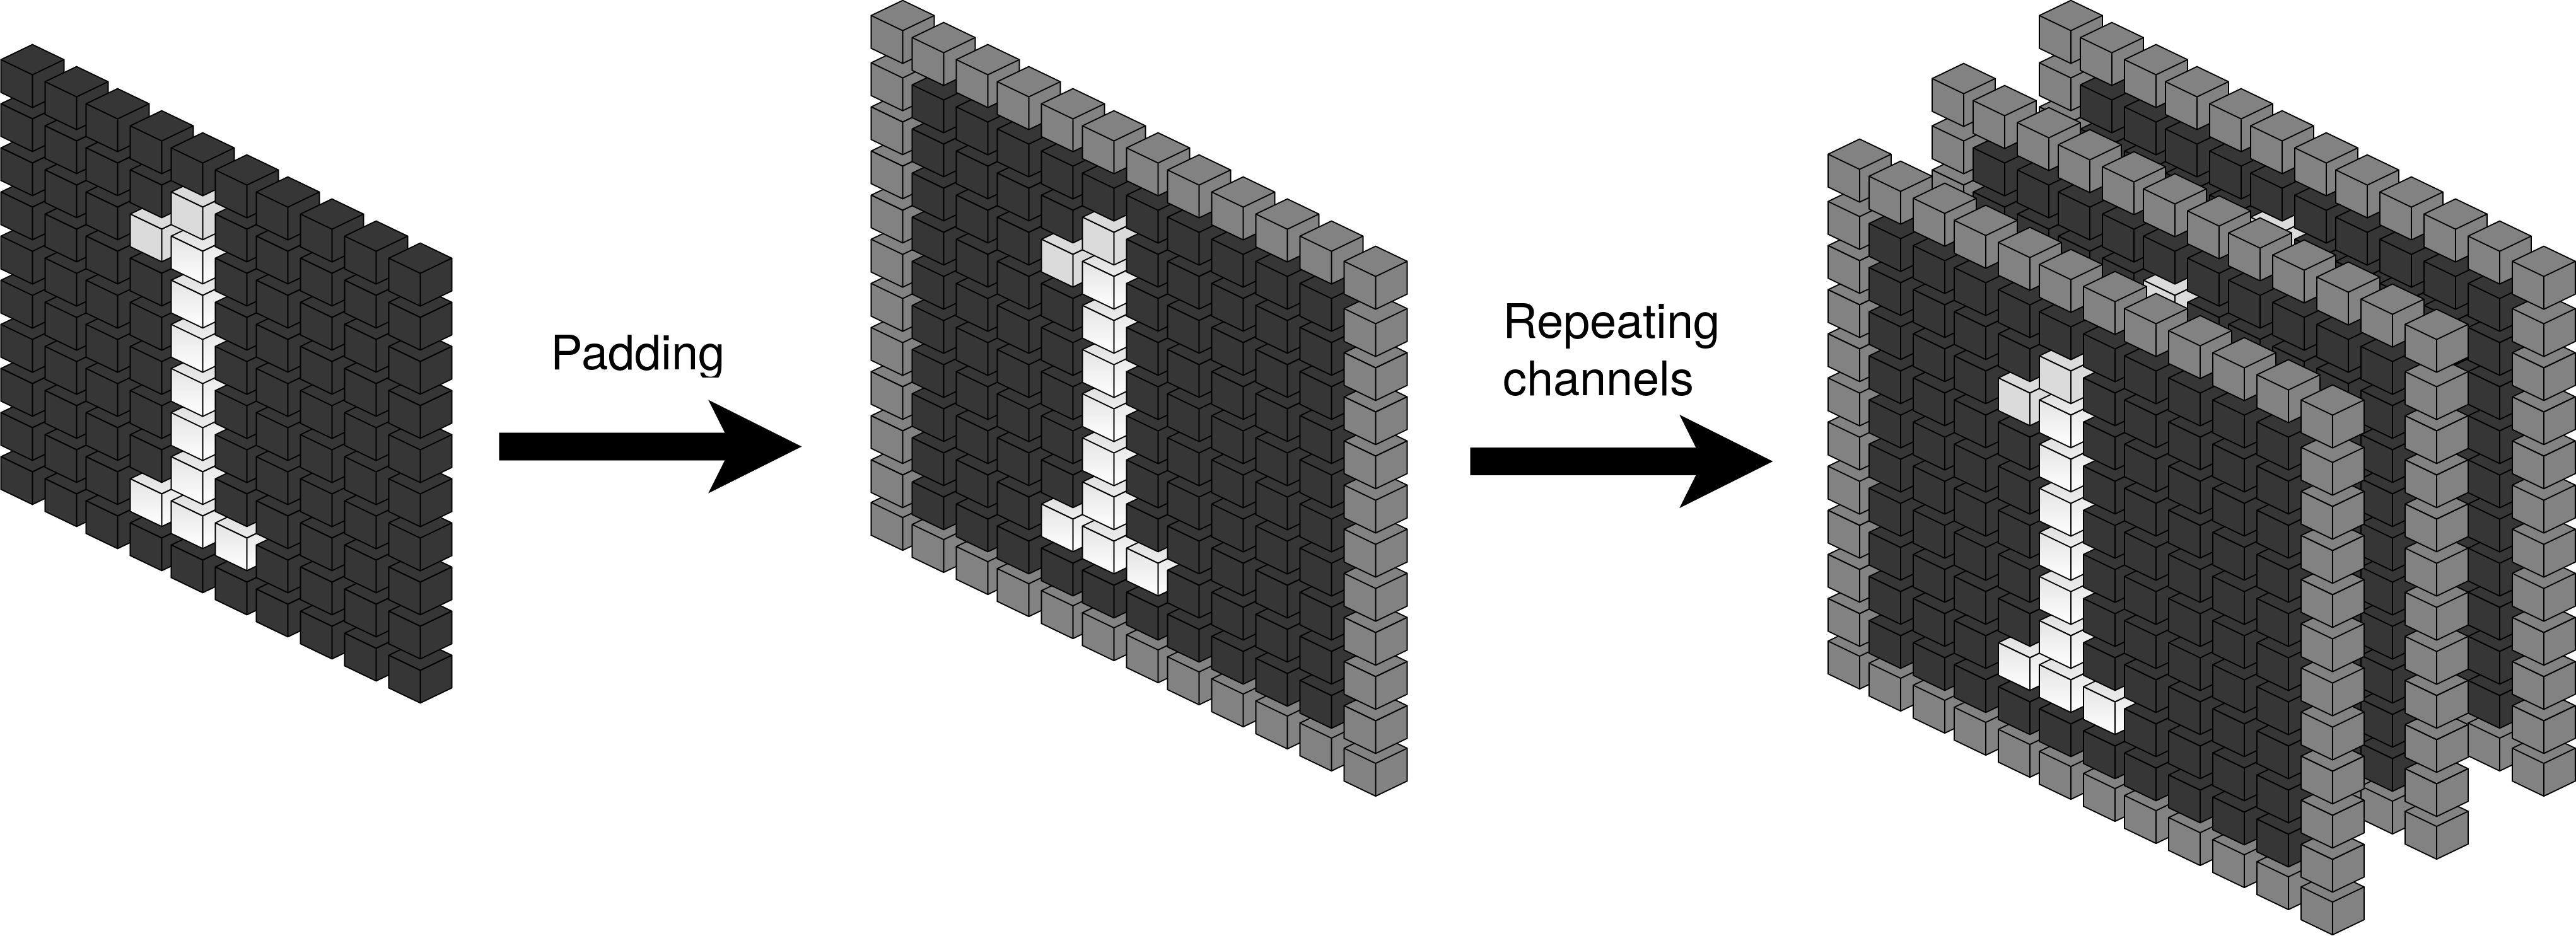
\includegraphics[width=\textwidth]{Chapters/4.Experiments/exp2/figures/MNISTpadding+repeating.png}
    \caption[MNIST modifications]{How MNIST is adapted to have same dimensions as cSVHN. Illustration use dimensions 12x12x3 while cSVHN and adapted MNIST use 32x32x3}
    \label{fig:MNISTpadding}
\end{figure}

\subsection{Tournament Search}\label{exp2:implementation.search}
The tournament search uses a population size of 64, and as discussed, a winner-replaces-all replacement scheme between generations. Instead of using a accuracy threshold as in the previous experiments, the search terminates after 100 generations. A important feature of PathNet is the way learning is done. Since network back propagation occur during path fitness evaluation, the locked number of generations limit the amount of training that is allowed. In the original paper, fitness is set as the negative training error which is reached for each path after it have been trained for one training unit of 50 mini batches of size 16. This is an reasonable way of evaluating the fitness of a path when using a small tournament size, but as the tournament size have been increased tenfold for the algorithms with high selection pressure, fitness is calculated differently in these experiment. 

The problem of directly using the training error as fitness is that the error changes whenever weights along a path is updated. An extreme example can be used to present the underlying problem with this.

\begin{figure}[ht]
    \centering
    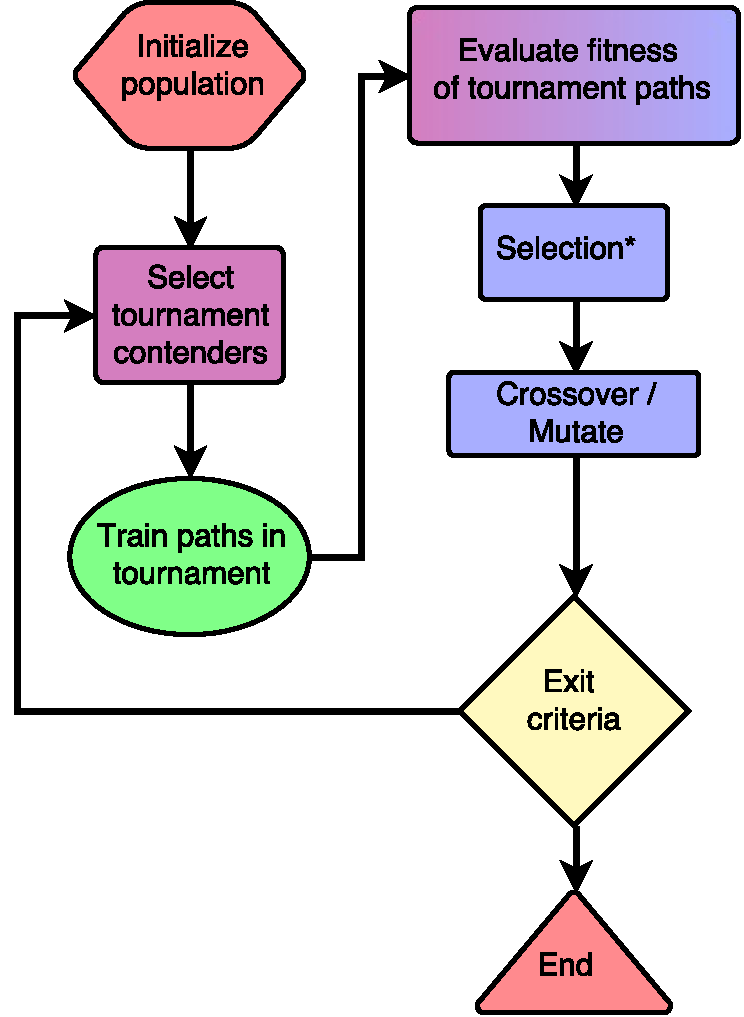
\includegraphics[width=0.5\textwidth]{Chapters/4.Experiments/exp2/figures/TS_implementation.pdf}
    \caption[Tournament search flowchart]{Flowchart of the tournament search implemented here. Compared to the flowchart of standard Tournament Search implementation in figure \ref{fig:algorithmflowcharts}, the difference is the extra step of training (green) before the fitness is evaluated. *The selection function always selects the tournament winner, except during algorithm 1c where the top two paths is selected.}
    \label{fig:ts_flowchart}
\end{figure}

Take a tournament selection of 25 genomes containing 24 identical paths and one different path with some module overlap to the others and which is evaluated first. One scenario could be that the first unique path is evaluated to a high fitness, when the next path evaluated, the weights in the modules which overlap between the two are updated. The evaluated fitness of the first path is now outdated, and for every subsequent path, this fitness might get worse and worse if the parameters in the overlapping modules move to an area of high error in the context of the first paths other modules. After all fitness evaluations, the first path now stands with a high fitness, which might be larger than that of all other paths in the tournament. Then all other paths in the tournament is replaced with the winning path even if its actual fitness might have become significantly reduced during the evaluation step. Due to this, the fitness of paths in a tournament is calculated in a separate step for these experiments as seen in figure \ref{fig:ts_flowchart}. After a subset of the population is selected for a tournament, all paths in that tournament are trained for one training unit. When training is completed, each path is evaluated by using a new subset of the training data for validation. This way, the order in which paths are validated does not affect the fitness score, which is the classification accuracy reached during the validation step. The order of paths still affect the the training but the fitness used for selecting a tournament winner is the "true"\footnote{Fitness is still calculated on the basis of the training data-set, which means it might become overly optimistic over time. Overfitting during training is discussed in the context of another experiment} fitness score.

The same reason influence the final step of the tournament search. When the limit of a hundred generations is reached, all paths in the population is evaluated again. Since the true fitness of a path might change from one generation to the next, only the paths participating in the final tournament has its true fitness score as part of the selection of the optimal path. As with the evaluation step, the final fitness of a path is the reached classification accuracy of one training unit (50 mini-batches of 16 samples). Using an actual validation set for this step might yield better, or at least more accurate, fitnesses to use as a basis for path-selection, but that would significantly increase the run-time of an already time intensive experiment. 

\section{Paths}
This section explores the results of the experimental trials where path-structure are in focus. 

\subsection{Results}
To test the effect algorithm choice has on path size, MWW tests (see appendix \ref{background:mannwhitney}) were run to test the null hypothesis that a pair of algorithms have the same path size distributionn. The resulting p-values are presented in the tables in section \ref{appendix:ptable.pathsize}. Using the Bonferroni corrected \(\alpha\) level of 
\begin{equation*}
    \alpha=\frac{\alpha_{desired}}{\text{number of MWW tests}}=\frac{0.05}{126}=3.968\time 10^{-4}
\end{equation*}
none of the null-hypotheses can be rejected, meaning the algorithm choice have no affect on path size. 

Also tested are the null-hypotheses that a algorithm A have the same distributions of total capacity used as a algorithm B for both A, B \(\in [1a, 1b, 1c, 2a, 2b, 3a, 3b]\) and A \(\neq\) B. Each algorithms capacity-use is also compared to the Monte-Carlo estimate, making 28 Mann-Whitney tests necessary. A significance level of \(\frac{0.05}{28}=1.7857\time 10^{-3}\) is therefore used. For this \(\alpha\) (or indeed a standard \(\alpha=0.05\). See table \ref{tab:exp2.capacityptable}) none of the algorithms were different from each other, but every algorithm was proved to be significantly different from the Monte-Carlo estimate of random capacity use. 

As a metric by itself, the capacity is influenced both by path-size and module reuse. All paths being equal, a high level of reuse for one algorithm would yield a significant difference in used capacity as the total number of used modules is reduced. As this is not observed we would expect the mean reuse for each algorithm to not contain significant differences.

\begin{sidewaysfigure}[p!]
    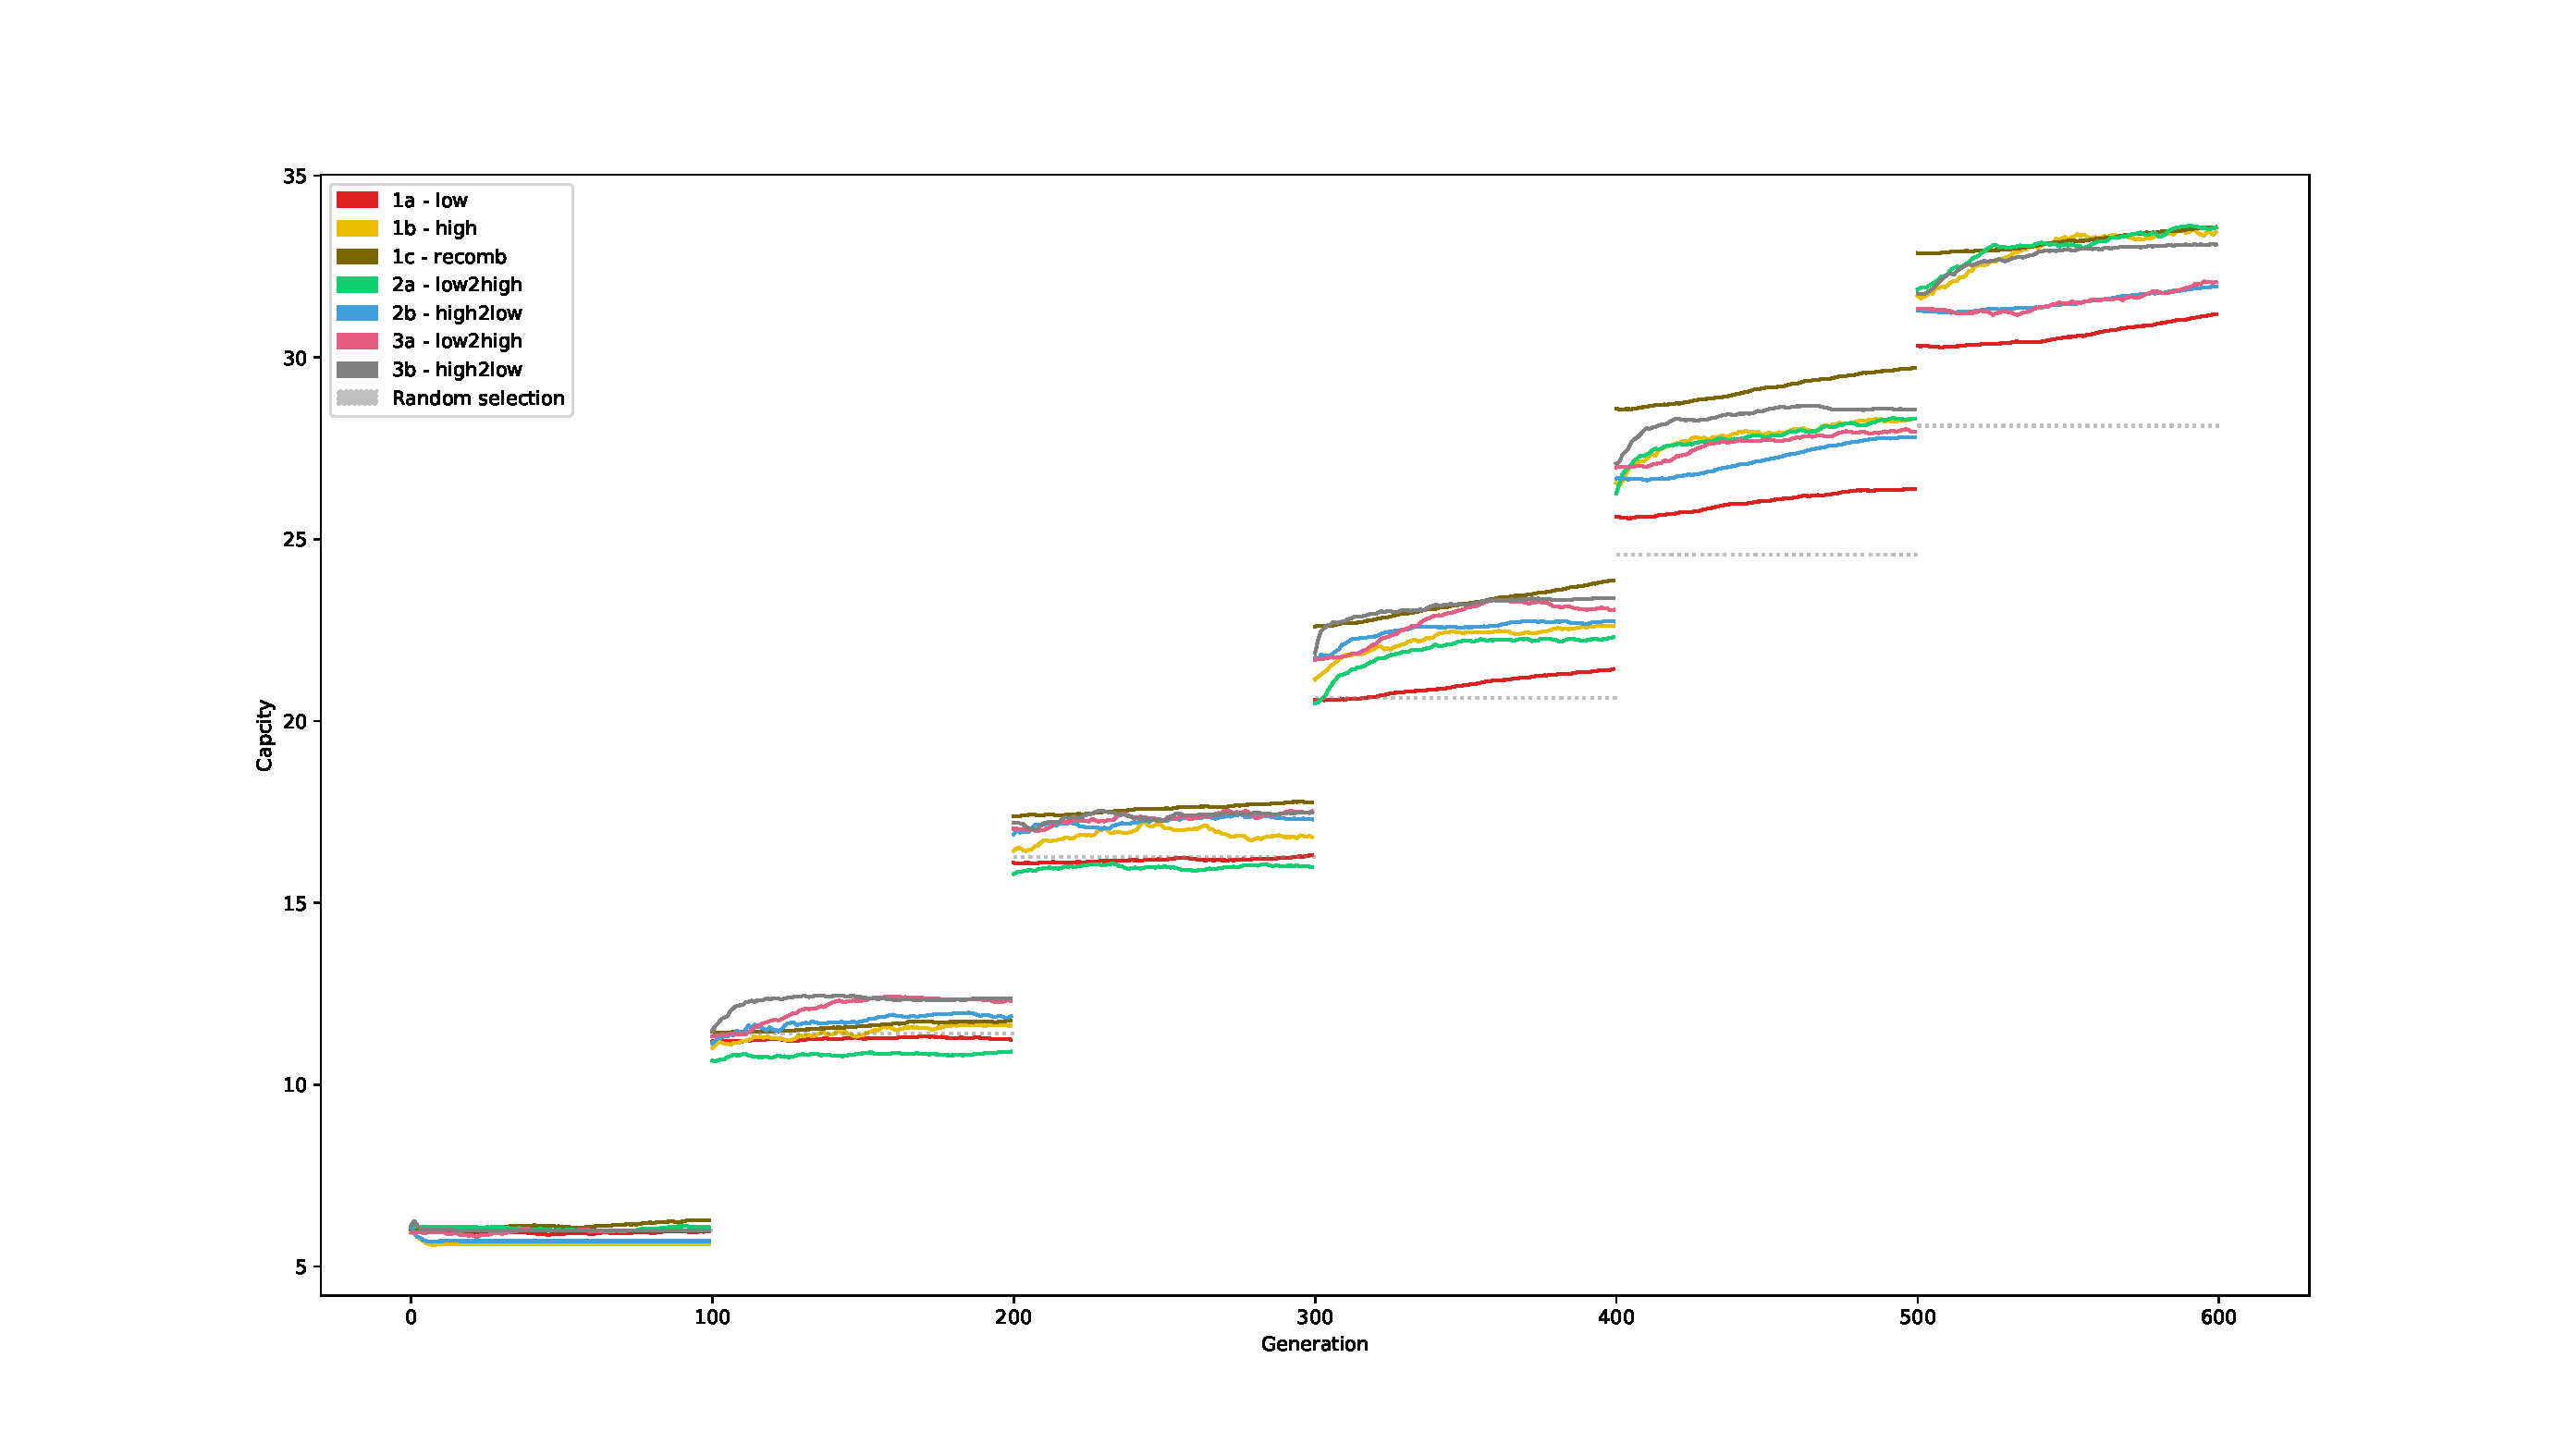
\includegraphics[width=1.2\textwidth,center]{Chapters/4.Experiments/exp2/figures/large/Capacity_pr_generation.pdf}
    \caption[Capacity plot]{The average number of used modules during the multi-task learning sequence. Each jump is caused by the saving of an optimal path and then starting a new search for a new task. }
    \label{fig:search.capacity}
\end{sidewaysfigure}

\begin{sidewaysfigure}[p!]
    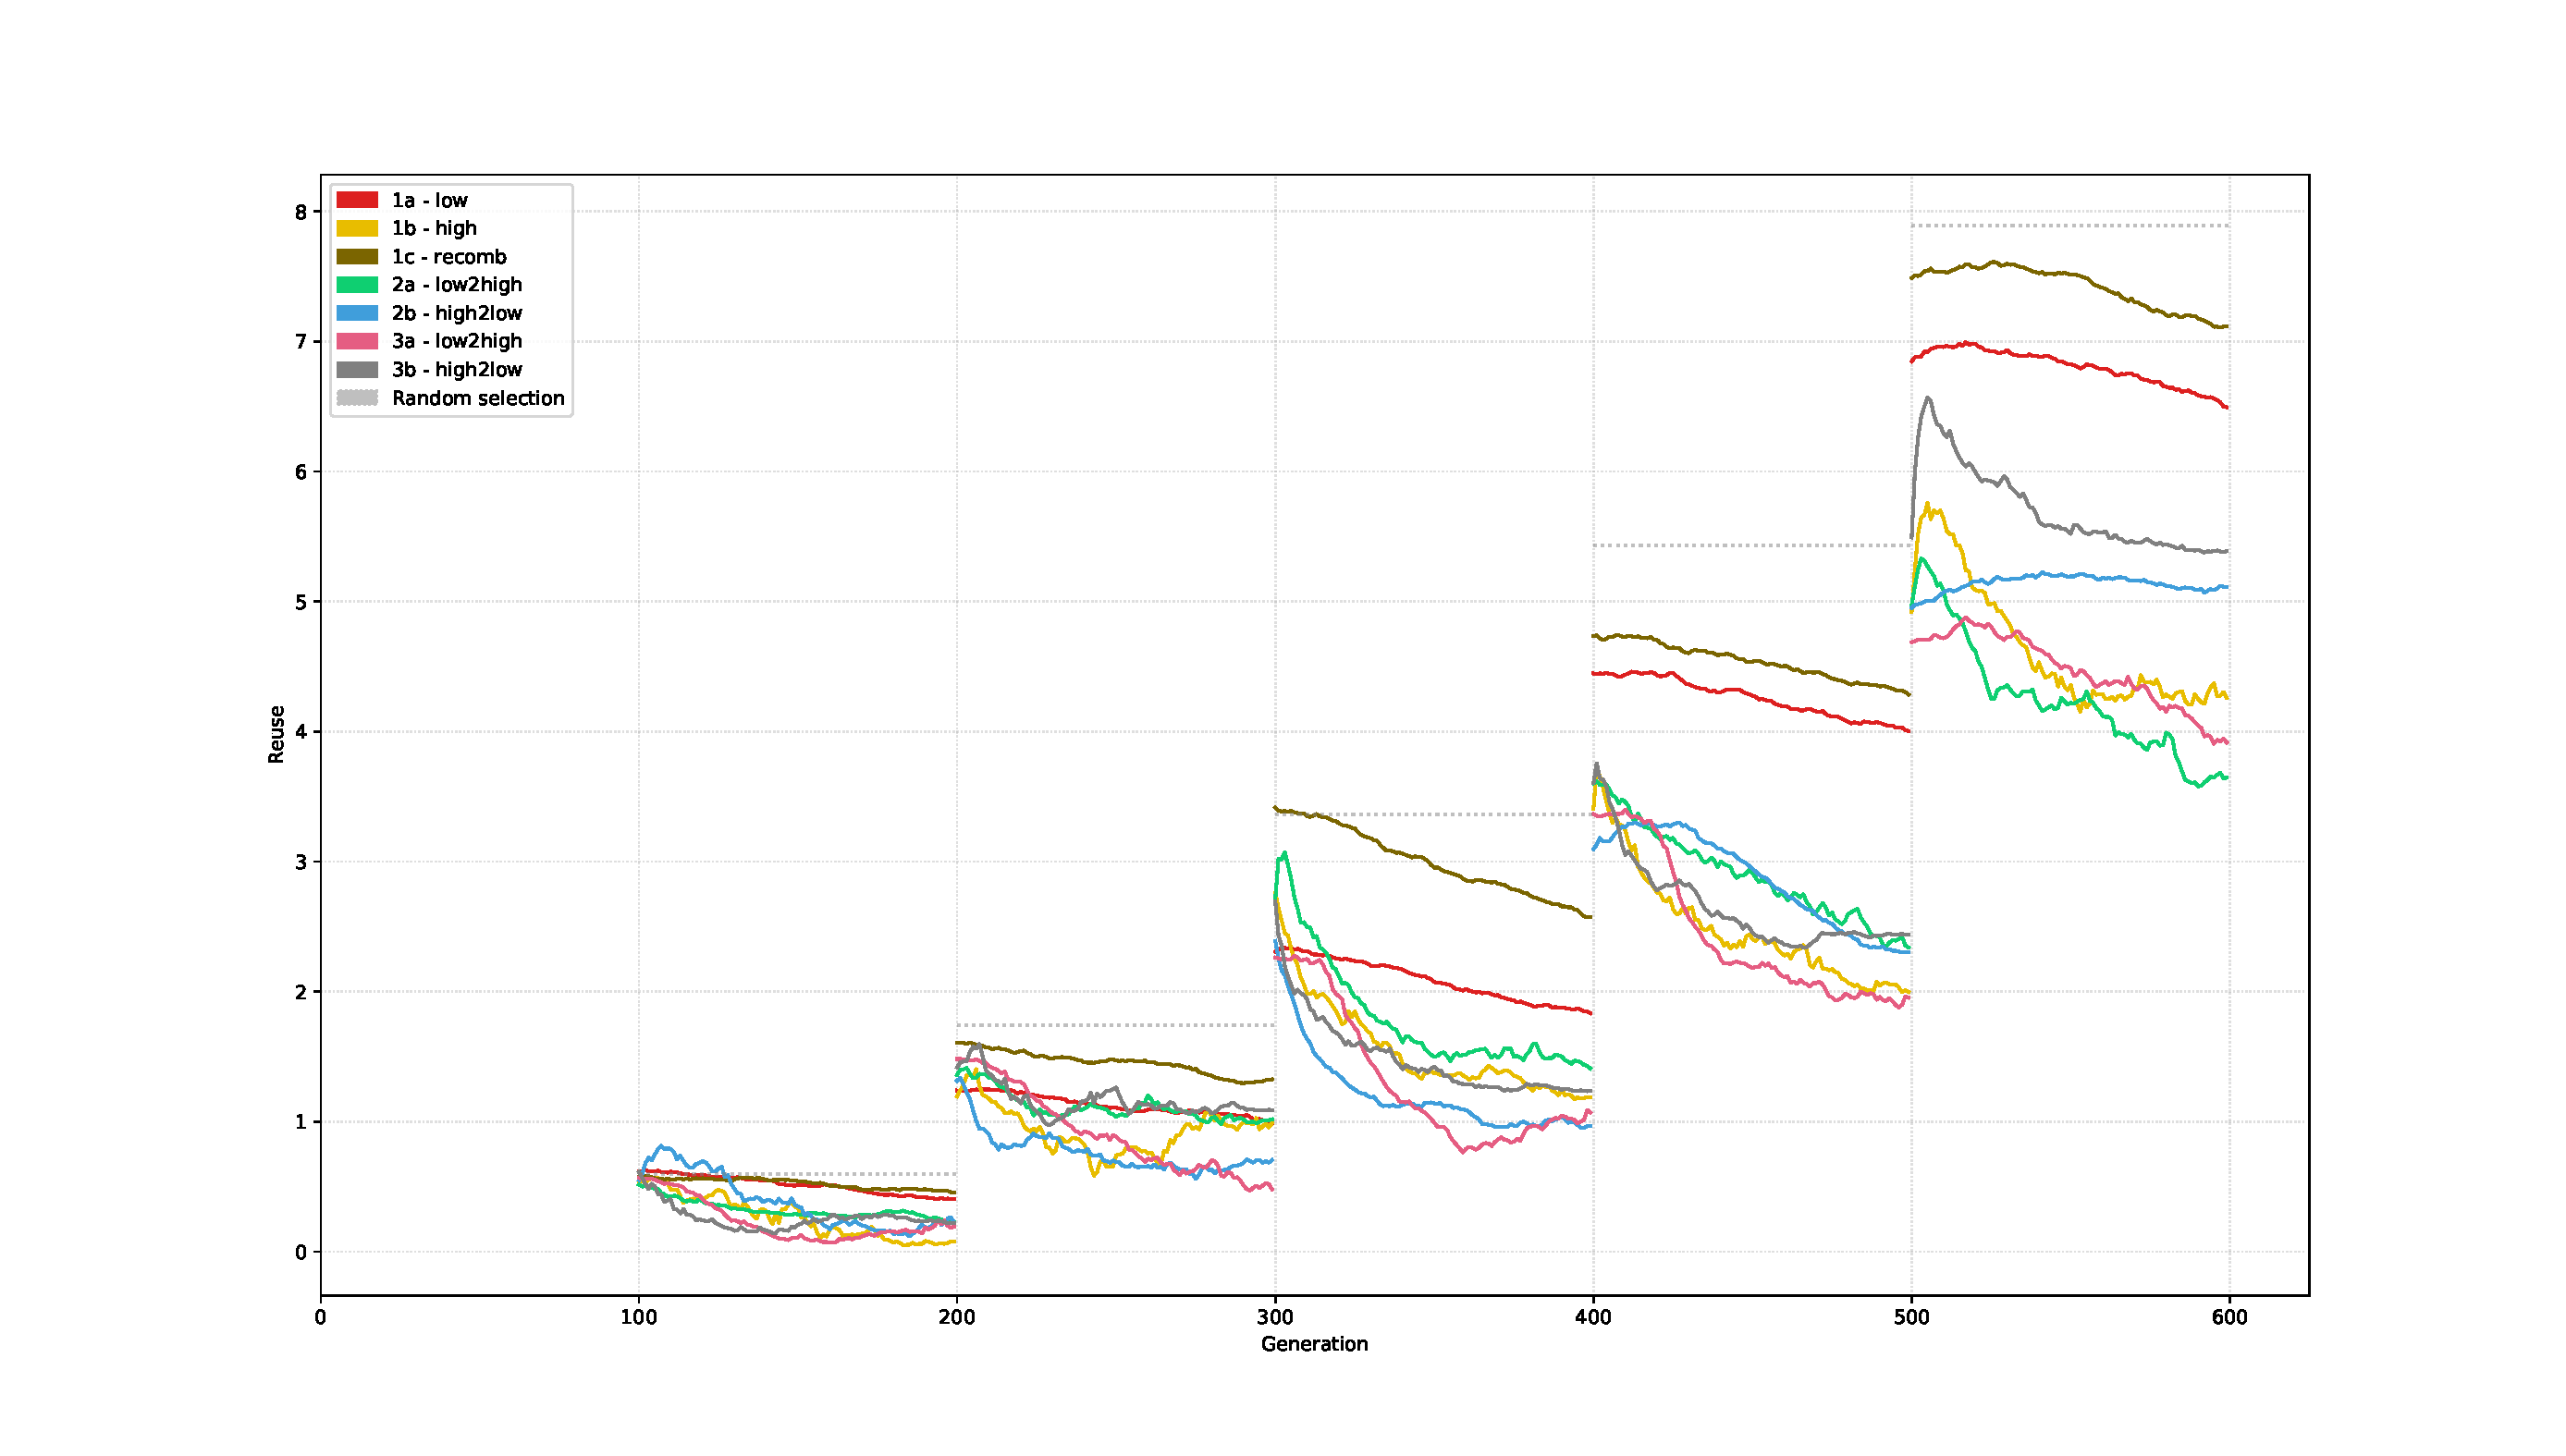
\includegraphics[width=1.2\textwidth,center]{Chapters/4.Experiments/exp2/figures/large/Module_reuse_pr_generation.pdf}
    \caption[Module reuse plot]{The average module reuse during the multi-task learning sequence. Each jump is caused by the saving of an optimal path, and the next task having more locked modules to reuse. The first 100 generations does not have any previously learned knowledge to reuse.}
    \label{fig:search.reuse}
\end{sidewaysfigure}

Figure \ref{fig:search.capacity} underlines the MWW results as there is only a small visual difference in average capacity between the algorithms.  Figure \ref{fig:search.reuse} on the other hand contain escalating fluctuations in the mean reuse across each algorithm. While all are below the Monte-Carlo estimated reuse, the algorithms seem to affect the change in reuse within each search differently. Another round of MWW tests however disproves this (see table \ref{tab:exp2.reuseptable}) as no null-hypotheses could be rejected under the Bonferroni corrected \(\alpha\)-level.

\subsection{Discussion}
While figure \ref{fig:search.reuse} show some differences, the results from these experiments seem to conclude that different tournament sizes does not have any effect on the selection of modules. The results seen here might be different for other tasks however, as a large difference in task difficulty could cause a PathNet with to little capacity to behave differently.

The Monte-Carlo estimation of reuse and capacity use was run for \(10^{6}\) trials, making the estimated value accurate to 4 decimal places if holding to a MSE 1 order of magnitude less than estimates (see formula \ref{eq:montecarloP}). It is noteworthy that the MWW-tests shows all algorithms being equal, but all algorithms performing significantly different from the Mote-Carlo estimates. This means we are seeing something similar to experiment in chapter \ref{exp1}, where the tasks were simple enough for modules to optimize quicker to training data than to the interface of pre-trained modules.

\section{Population diversity}\label{exp2:diversity}
\subsection{Results}
\ref{fig:search.hamming_diversity} visualizes the average population diversity for each algorithm for each task calculated with the pair-wise Hamming distance metric. 

\begin{sidewaysfigure}[p!]
    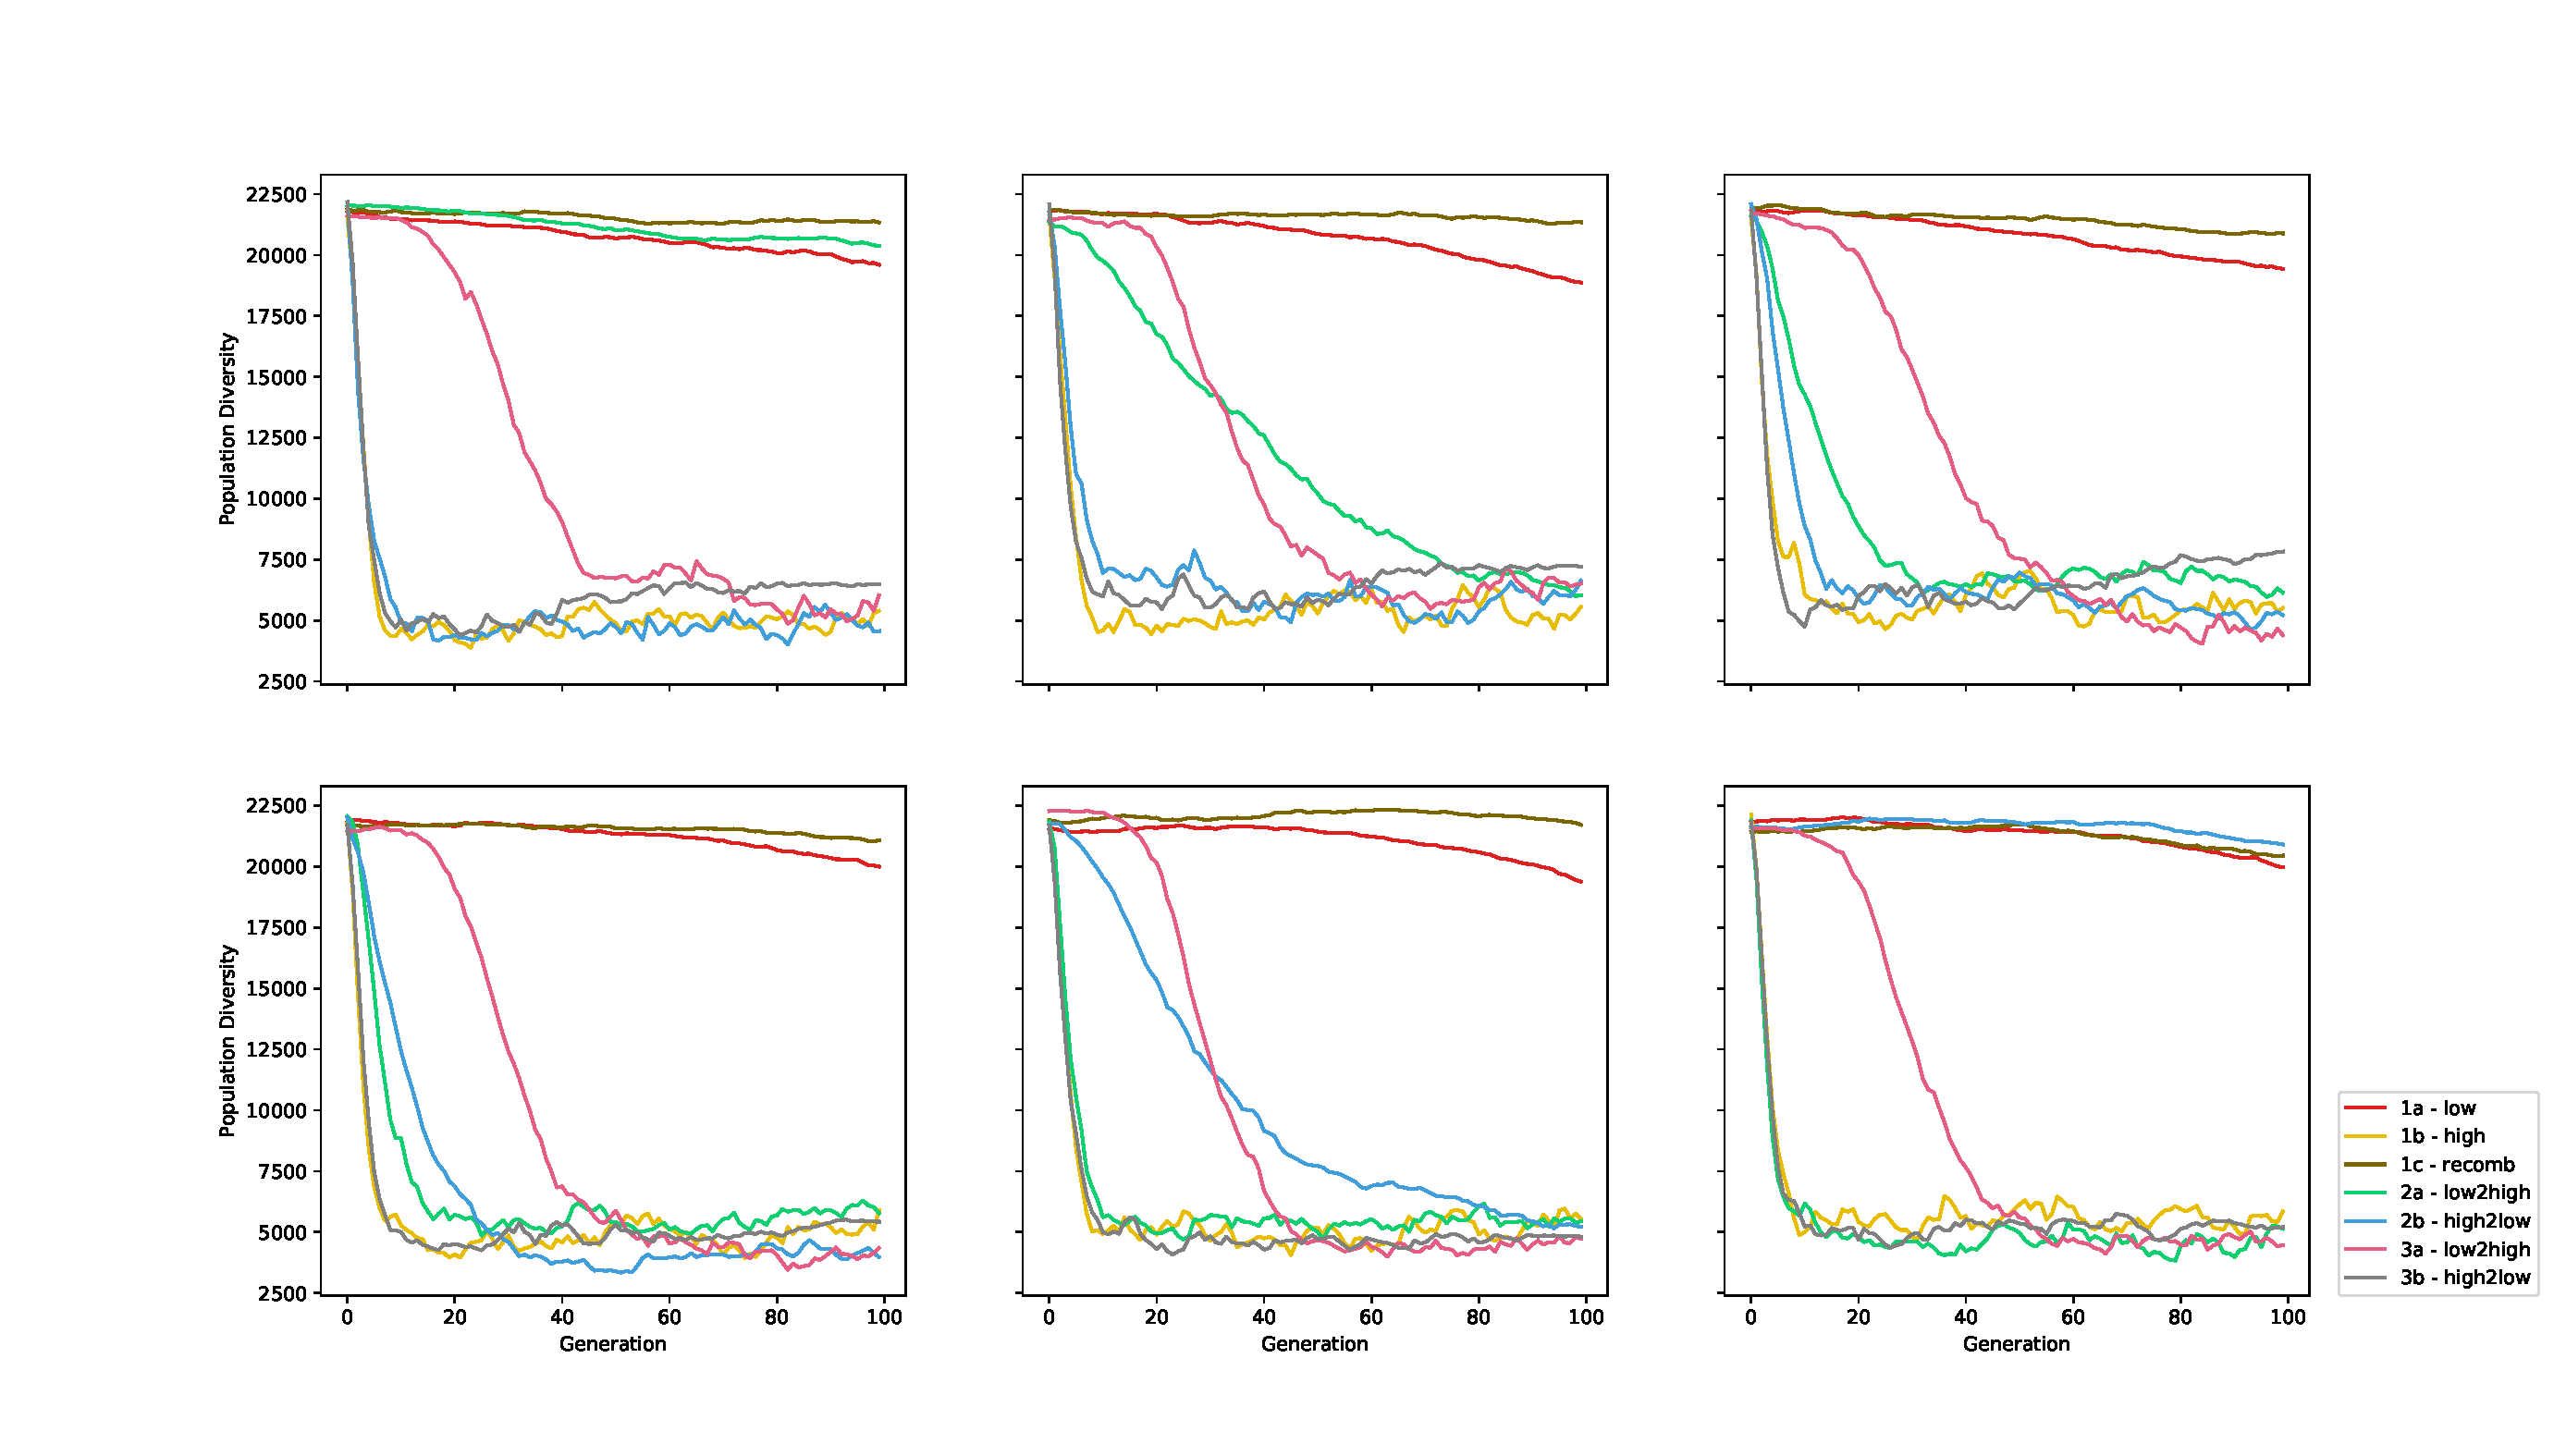
\includegraphics[width=1.2\textwidth,center]{Chapters/4.Experiments/exp2/figures/large/Average_population_diversity_reduced_hamming.pdf}
    \caption[Pair-wise Hamming distance diversity]{The average pairwise Hamming distance within each generation is used as a measure for population diversity. Each subplot (in order left to right) is each task in trained order.}
    \label{fig:search.hamming_diversity}
\end{sidewaysfigure}

When a generation is over and mutations of the tournament winner replace all losers, the population makes a large shift in diversity unless most of the tournament participants have a similar genome, at which point population have most likely converged. This is why all diversity plots (\ref{fig:search.hamming_diversity} and \ref{fig:search.frequency_diversity_unique}) contain rapid changes for sections of high tournament size, while algorithms 1a and 1c (also algorithm 2a for the first tasks, 2b for the later tasks) have more gradual changes. 

\begin{sidewaysfigure}[p!]
    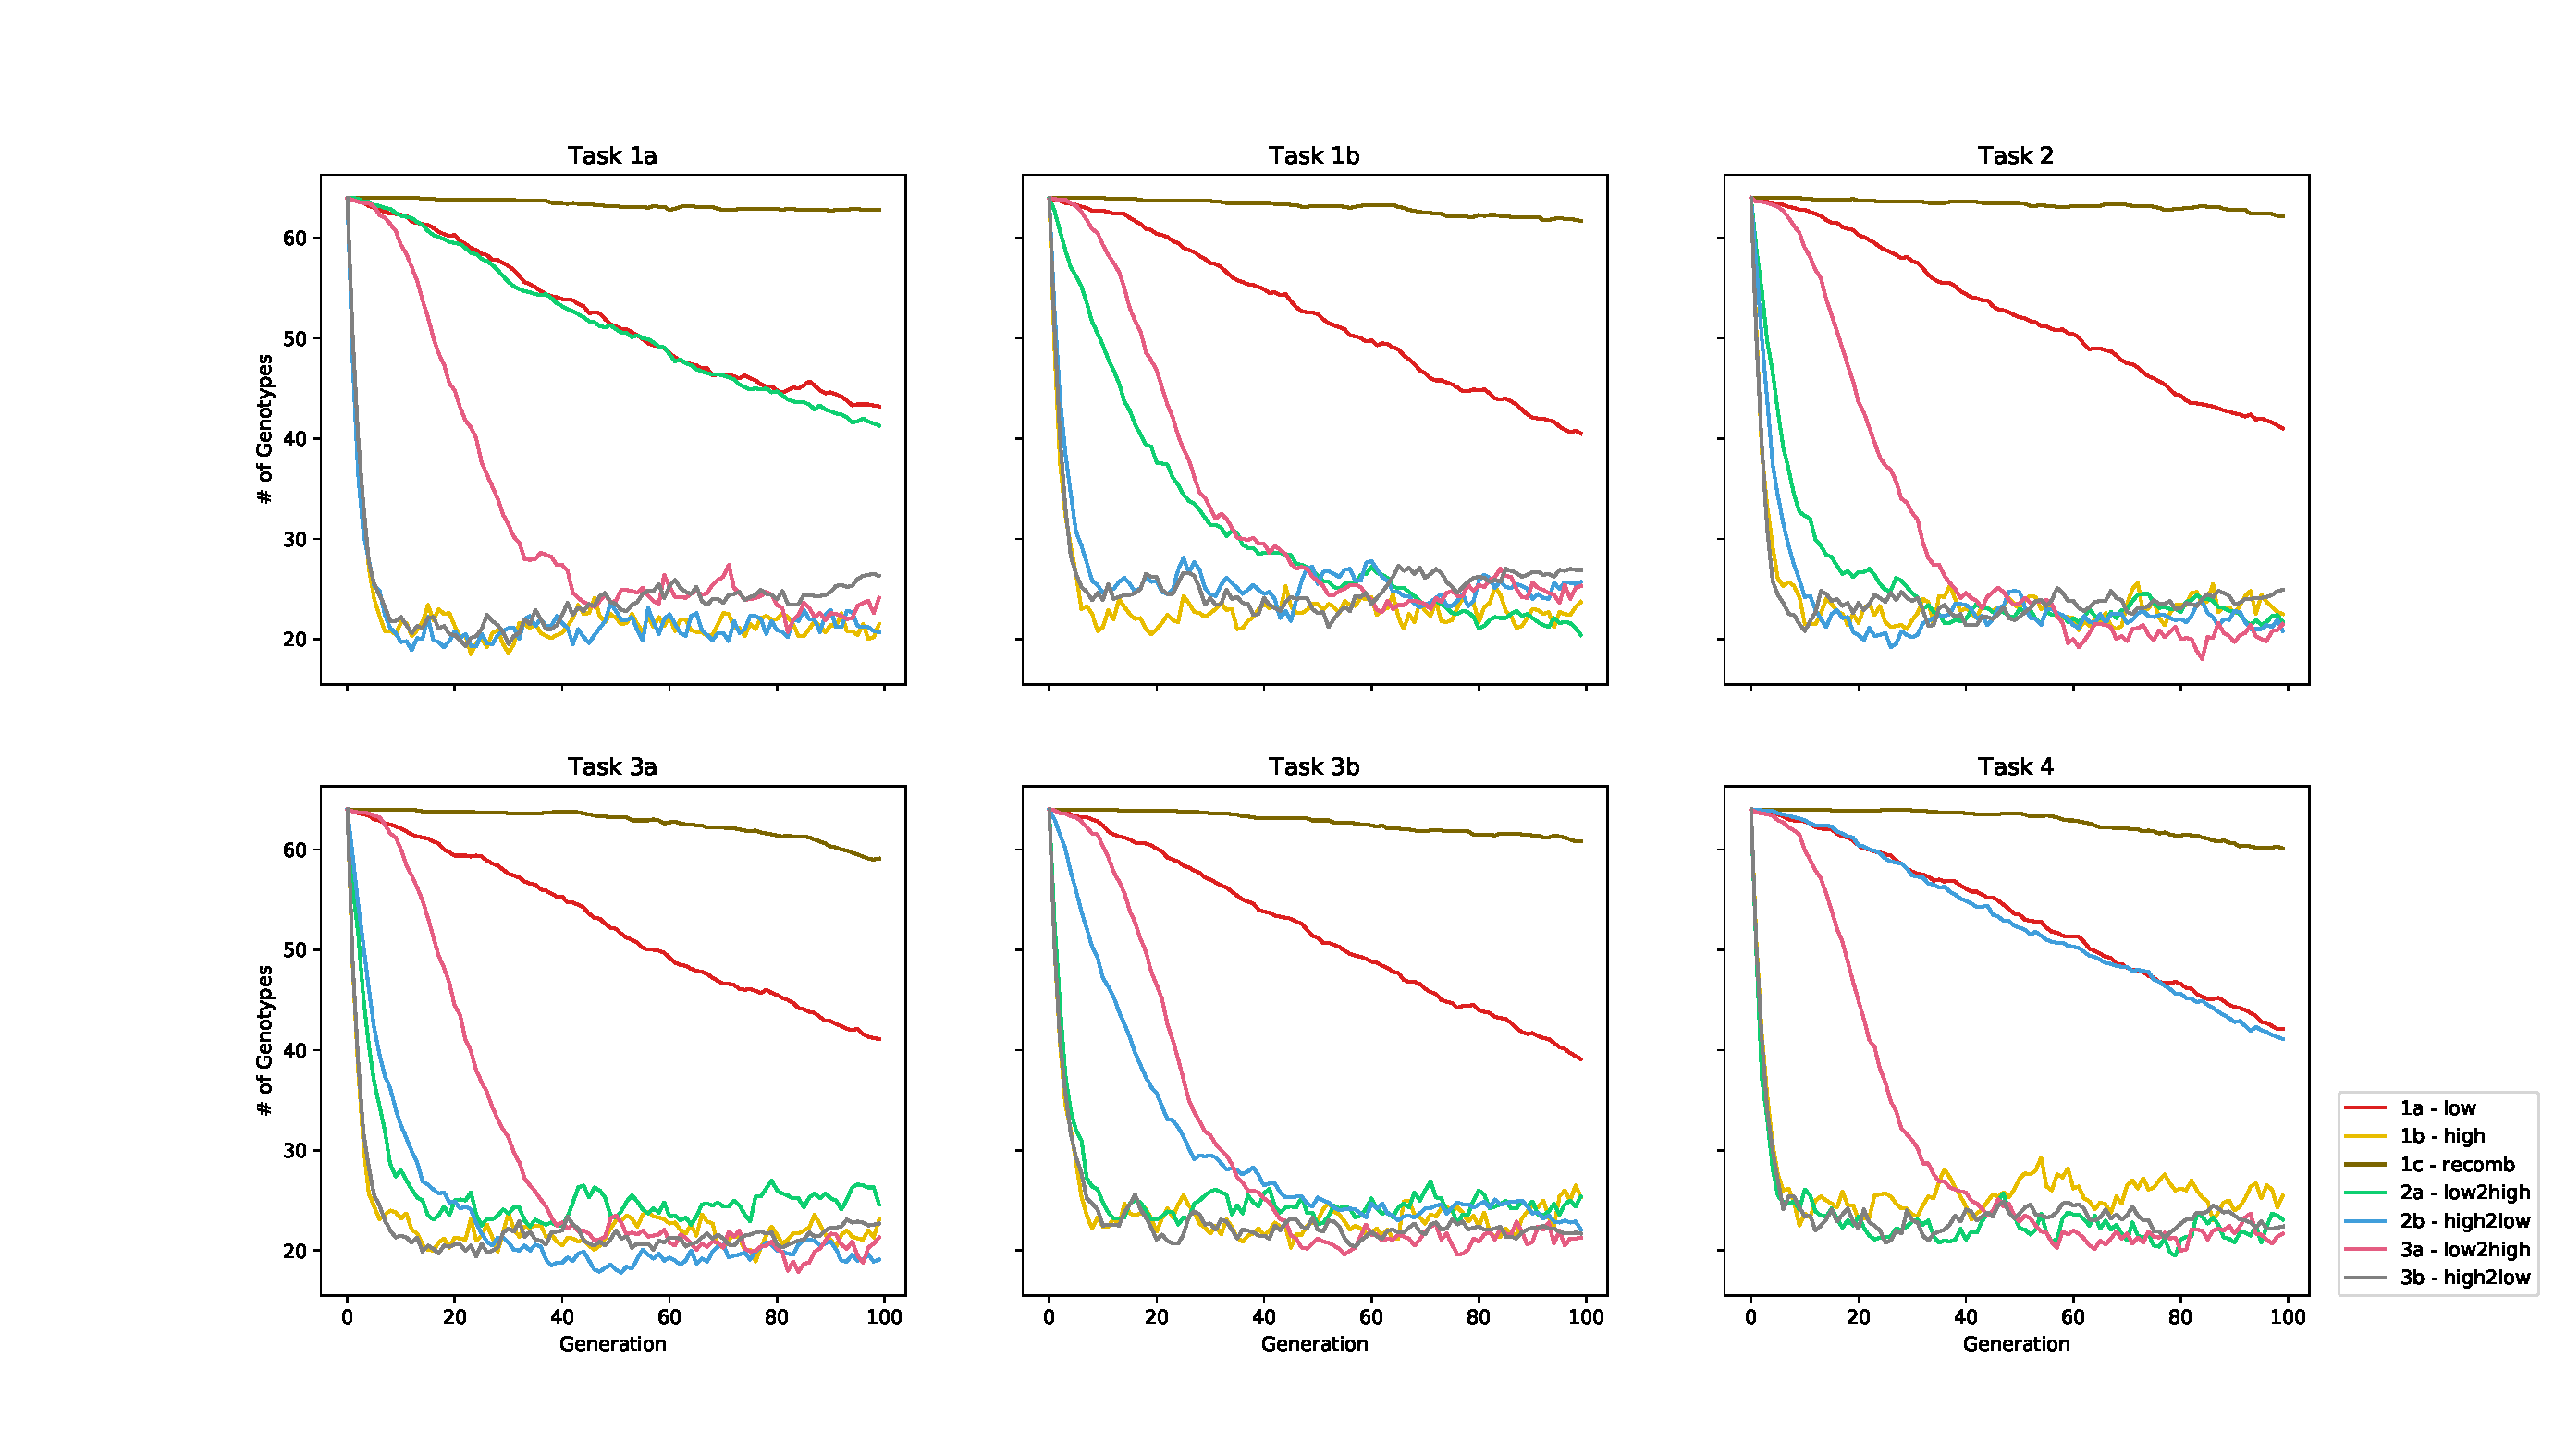
\includegraphics[width=1.2\textwidth,center]{Chapters/4.Experiments/exp2/figures/large/frequency_diversity_unique_path_count.pdf}
    \caption[Unique genome frequency diversity]{The number of unique paths within a population. Plotted for every task and every algorithm.}
    \label{fig:search.frequency_diversity_unique}
\end{sidewaysfigure}

Plots \ref{fig:search.hamming_diversity} and \ref{fig:search.frequency_diversity_unique} contain about the same information, and confirms the ordering of selection pressure is what was intended. The only difference worth mentioning is the one of algorithm 1a for the two plots. We would expect the frequency diversity to misrepresent tie diversity of a population as being higher than it actually is due to it counting small mutations as totally different genomes. Here we see frequency giving a smaller diversity than Hamming distance, which suggests Hamming distance is the one misrepresenting reality. 

Also note algorithms 2a and 2b. The convergence rate of these algorithms changes as the tournament size does. Comparing to algorithms 1a and 1b uncovers that tournament size 15, 20 and 25 gives no notable difference in convergence rate from algorithms 1b, while there is a small but visible difference for tournament size 10. Size 5 is the only one distinguishing itself from other tournament sizes or selection pressure schemes. 

Grouping by convergence rate would indicate tournament sizes 10, 15, 20 and 25 are equal to each other and algorithm 3b. 3a is much the same as tournament size 5. 1a is slow but steadily converging and would most likely do so if the generation termination limit was increased, while 1c shows no such tendencies. 

\subsection{Discussion}
As hypothesized, low tournament size yielded low convergence rate while high tournament size gave high convergence. Figures \ref{fig:search.hamming_diversity} and \ref{fig:search.frequency_diversity_unique} also makes it possible to rank the algorithms by its selection pressure on a \textit{"exploration vs. exploitation"} scale. Algorithms 2a and 2b change throughout the multi-task scenario, and their selection pressure follow this change. Algorithms 3a and 3b however behave the same for each path-search. From the plots it is obvious that algorithm 3a has a lower convergence rate than 3b, as its tournament size starts out small and grows during the search. I.e: algorithm 3a has a lower selection pressure than algorithm 3b. 

Looking at algorithms 2a and 2b in figures \ref{fig:search.hamming_diversity} and \ref{fig:search.frequency_diversity_unique}, it seems the tournament size does not scale linearly with convergence. Tournament sizes 10, 15, 20 and 25 have similar convergence rate to that of algorithm 1b. This would indicate that a static tournament size of 10 would provide similar exploration and exploitation to a path search as a tournament size of 25. 

While both algorithm 1a and 1c have low selection pressure and therefor also a low convergence rate, figure \ref{fig:search.frequency_diversity_unique} has a especially poor description of the diversity of algorithm 1c. The recombination functionality ensures the offspring of two genomes is genetically different from both parents even though the overall genetic diversity have dropped.

\section{Training}

\subsection{Results}

\begin{sidewaysfigure}[p!]
    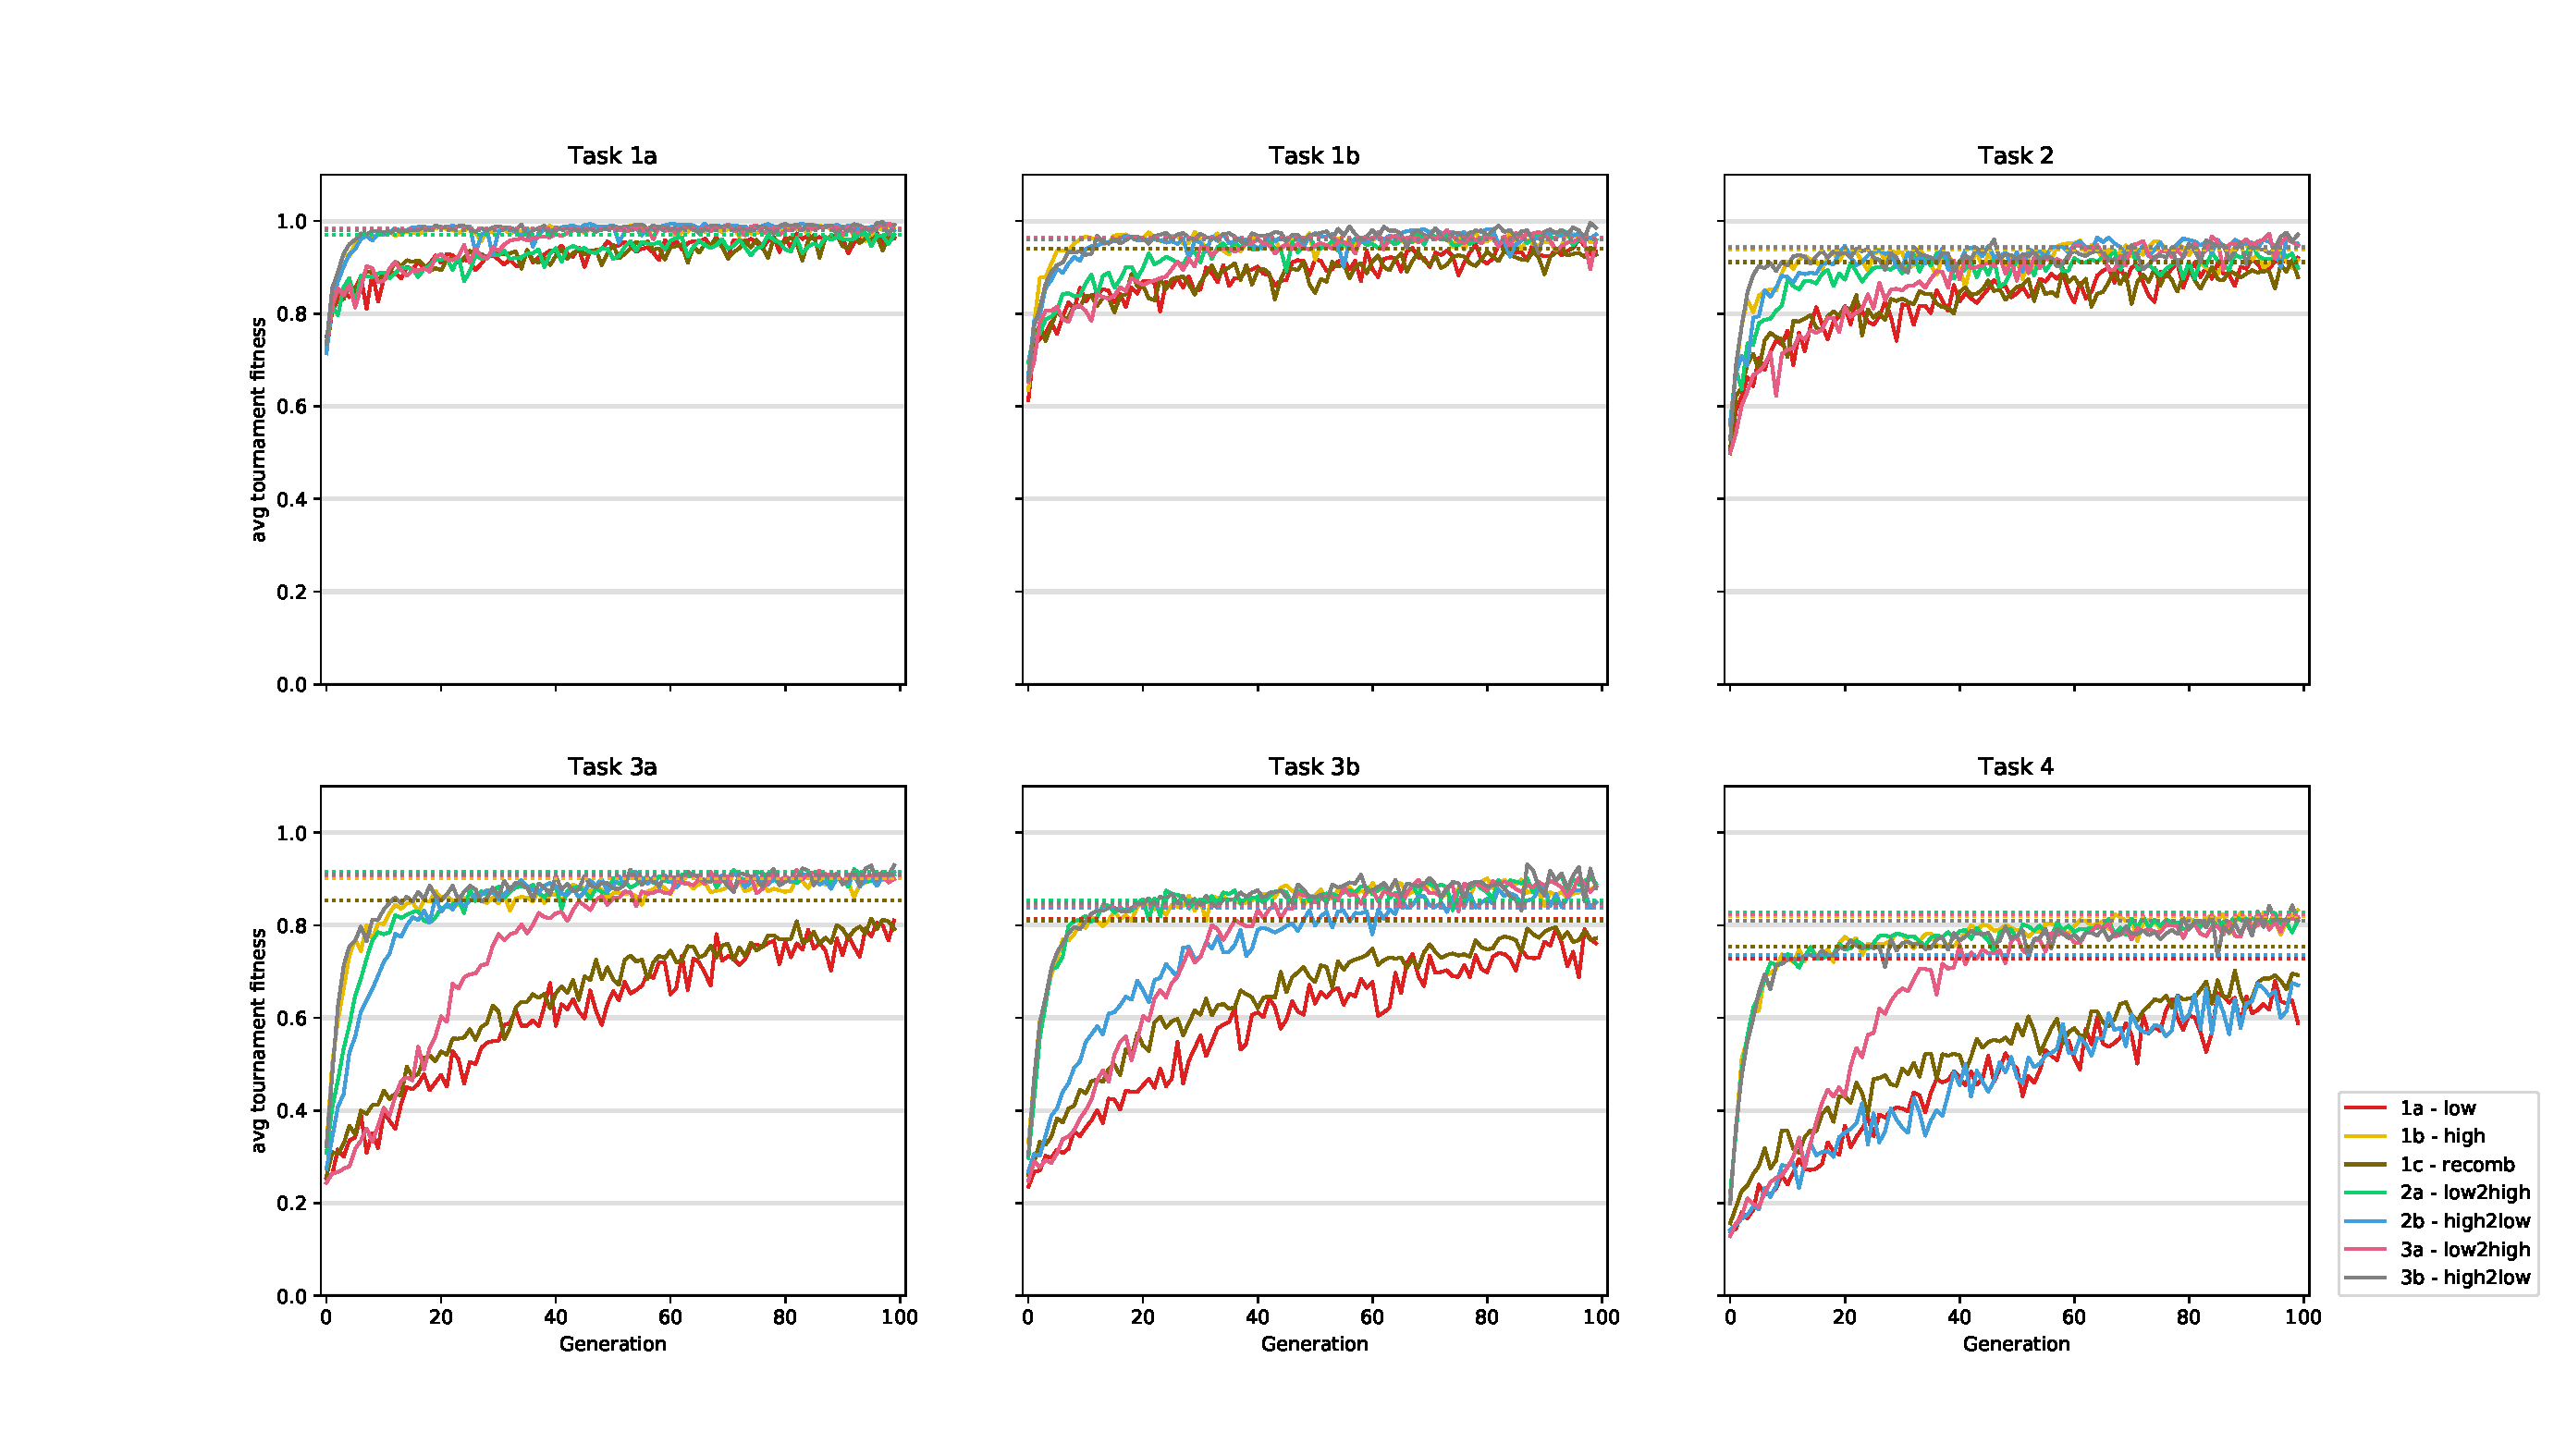
\includegraphics[width=1.2\textwidth,center]{Chapters/4.Experiments/exp2/figures/large/Training_accuracy.pdf}
    \caption[Fitness plot]{Average fitness during search. The dotted lines is the average achieved validation accuracy for that task and that algorithm.}
    \label{fig:search.accuracy}
\end{sidewaysfigure}

As the training of each path is done during and controlled by the search, how the average training accuracy develops gives an indication of how quickly the algorithms are able to influence the overall PathNet to learn a task. As discussed in section \ref{exp2:implementation.search}, the act of training one tournament of genomes affect the previously evaluated fitness values. Because of this, the populations average fitness value would be a highly misleading metric to use and therefore what is plotted in figure \ref{fig:search.accuracy} is the average fitness score achieved within a each generations tournament. Also plotted is the mean validation accuracy reached for each algorithm. This validation score is only calculated after an optimal path have been found for each task, and can therefore not be viewed as a function of generation number. The validation accuracy is visualized separately as a box-plot in figure \ref{fig:search.validation}.

\begin{sidewaysfigure}[p!]
    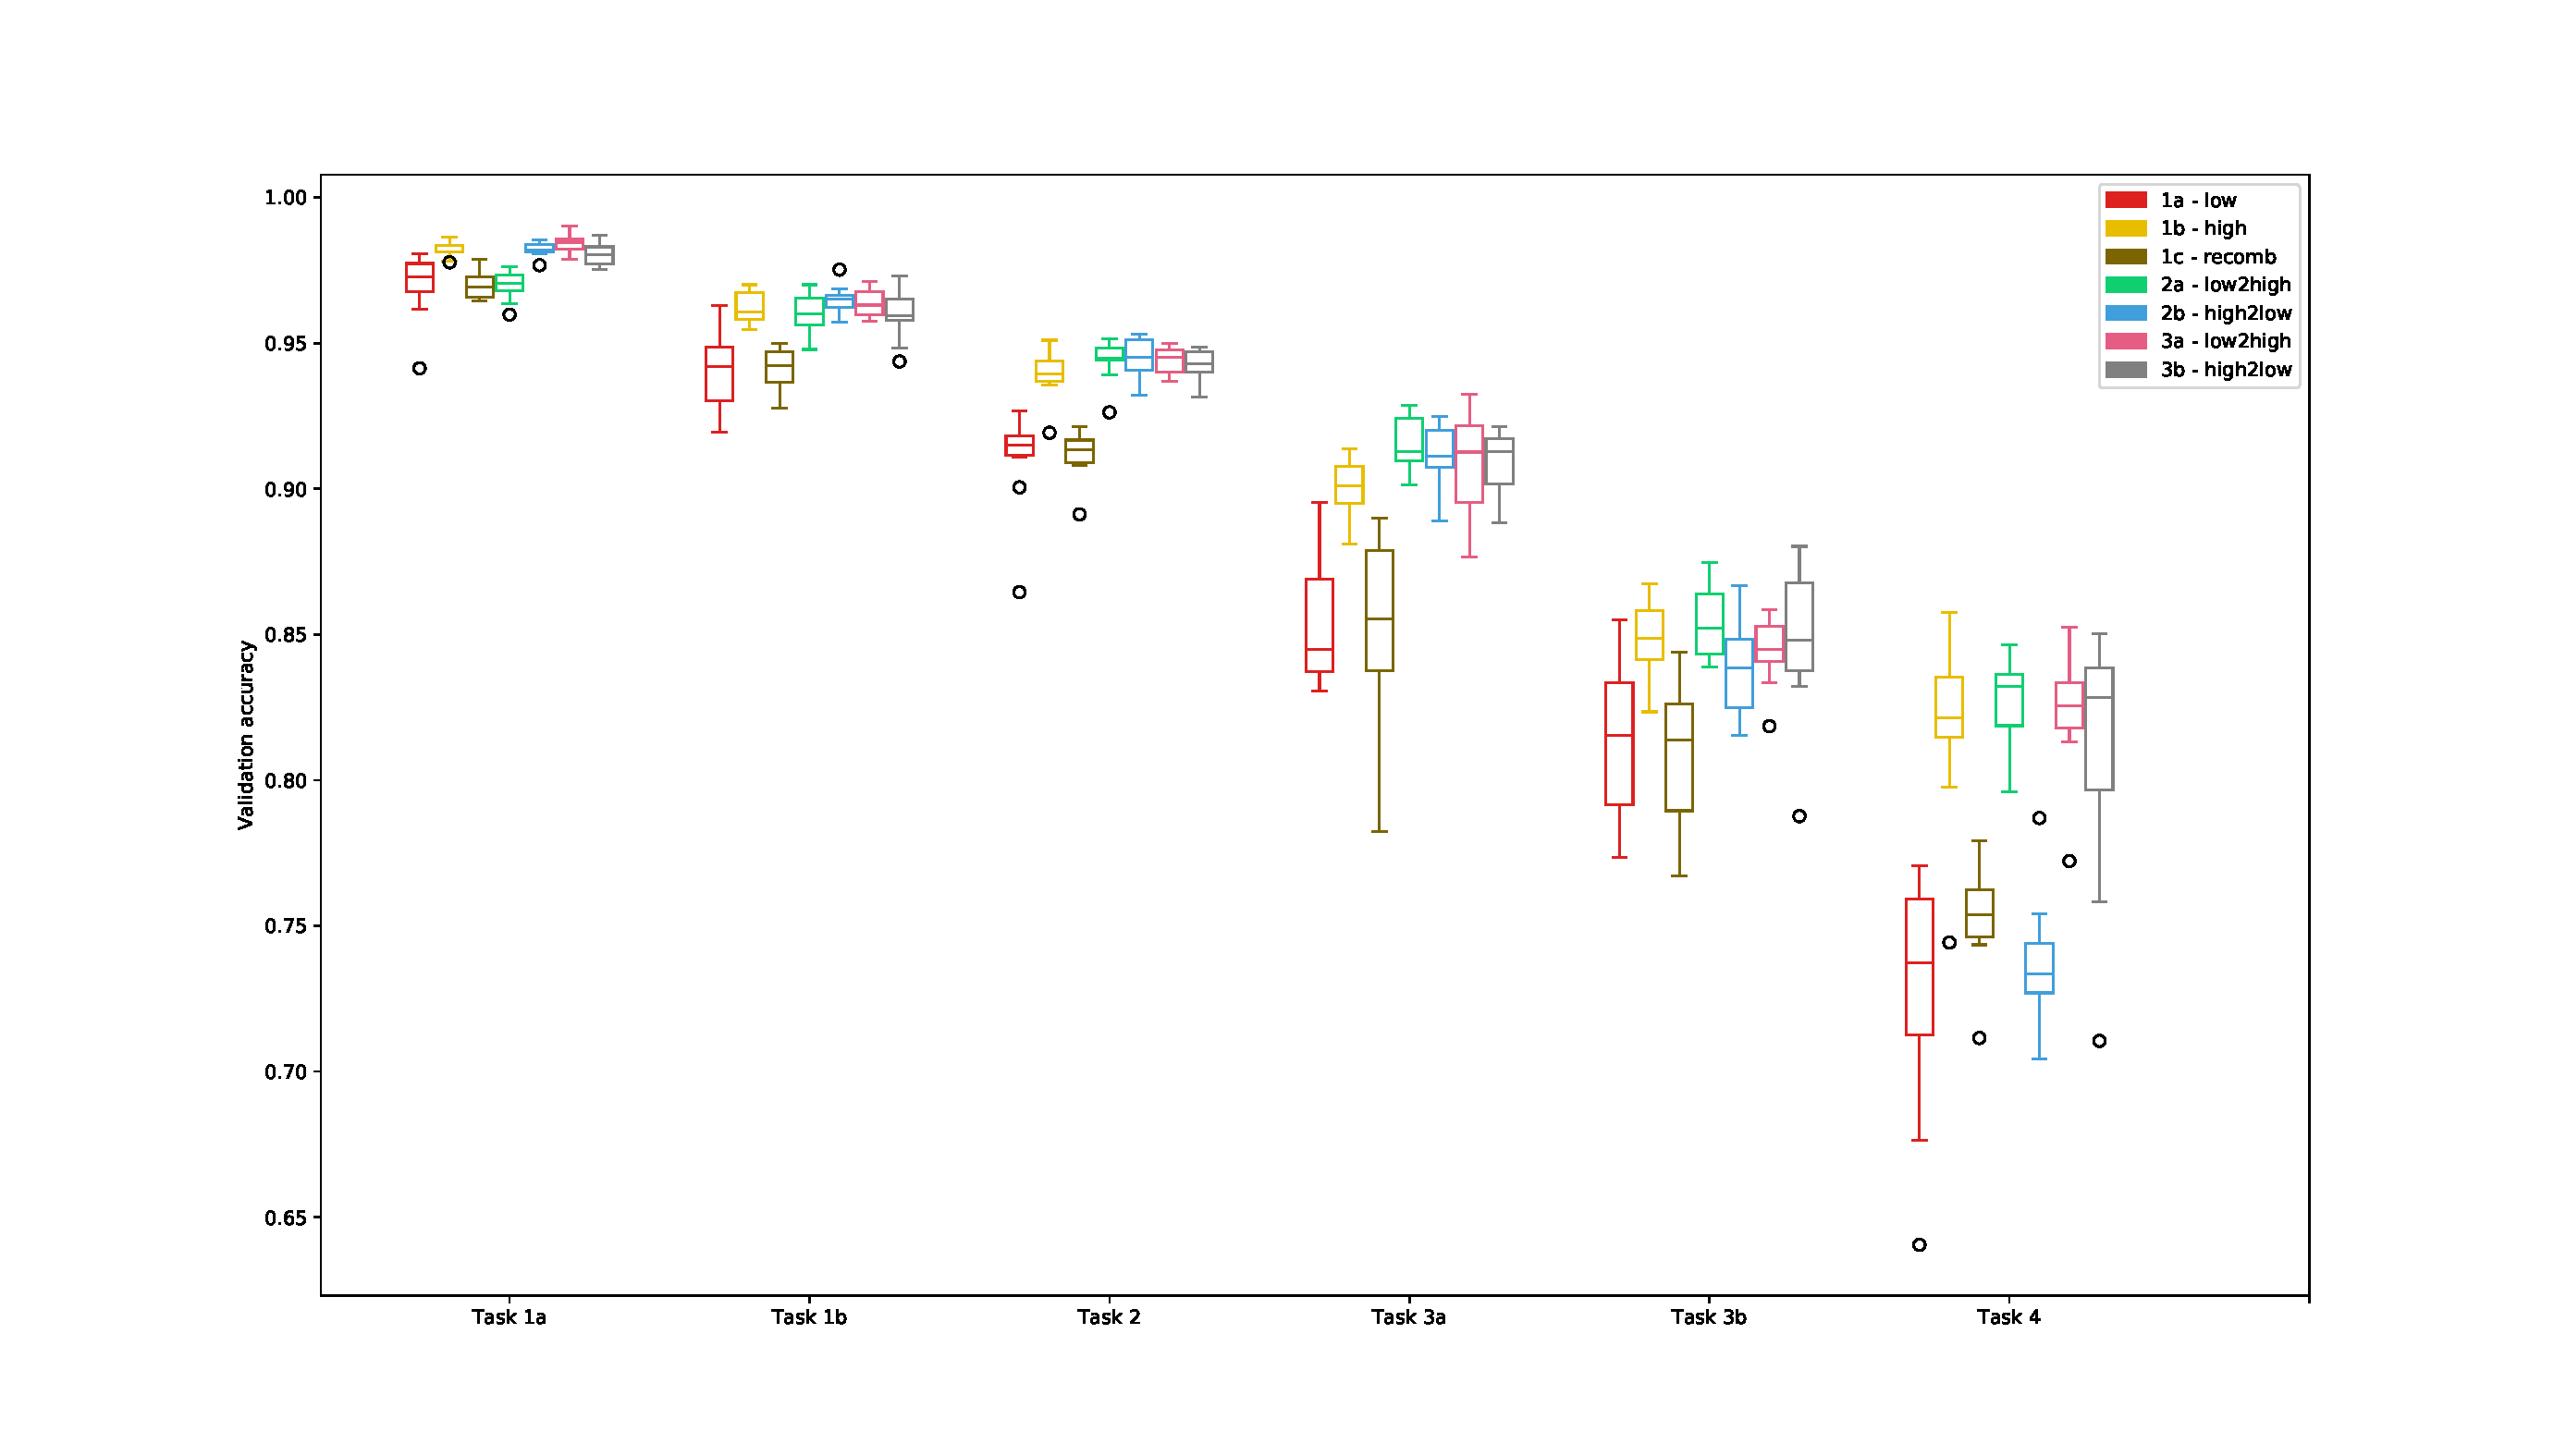
\includegraphics[width=1.2\textwidth, center]{Chapters/4.Experiments/exp2/figures/large/validation_boxplot.pdf}
    \caption[Validation accuracy plot]{Boxplot of validation accuracy reached for each task and each algorithm.}
    \label{fig:search.validation}
\end{sidewaysfigure}

Again, one MWW-test is run for every pair of algorithm for each task, this time to test the distributions of validation accuracies under the \(\alpha\)-level 0.0003968. Comparing this \(\alpha\) to results in tables in section \ref{appendix:ptable.accuracy}, some patterns emerge: 
\begin{itemize}
    \item Low tournament size: There is no significant difference in accuracy distribution between the algorithms with static low tournament size. The algorithms 2a and 2b are also similar to 1a and 1c for those tasks where they have a low tournament size. Meaning task 1a for algorithm 2a and task 3b and 4 for algorithm 2b. 
    \item High tournament size: Algorithm 1b is only significantly different from other algorithms when they use a tournament size of 2 or 3, the exception being algorithm 1a for task 3b and 4, where the null-hypothesis can not be rejected. 
    \item Changing tournament size: Algorithms 2a and 2b differ significantly only when their tournament size is most different; tasks 1a and 4. 
    \item Dynamic tournament size: Algorithms 3a and 3b does not differ for any task, and are also similar to algorithm 1b for all tasks. They do seem to differ from the low tournament size algorithms for most tasks however, except task 3b. 
\end{itemize}

\begin{sidewaysfigure}[p!]
    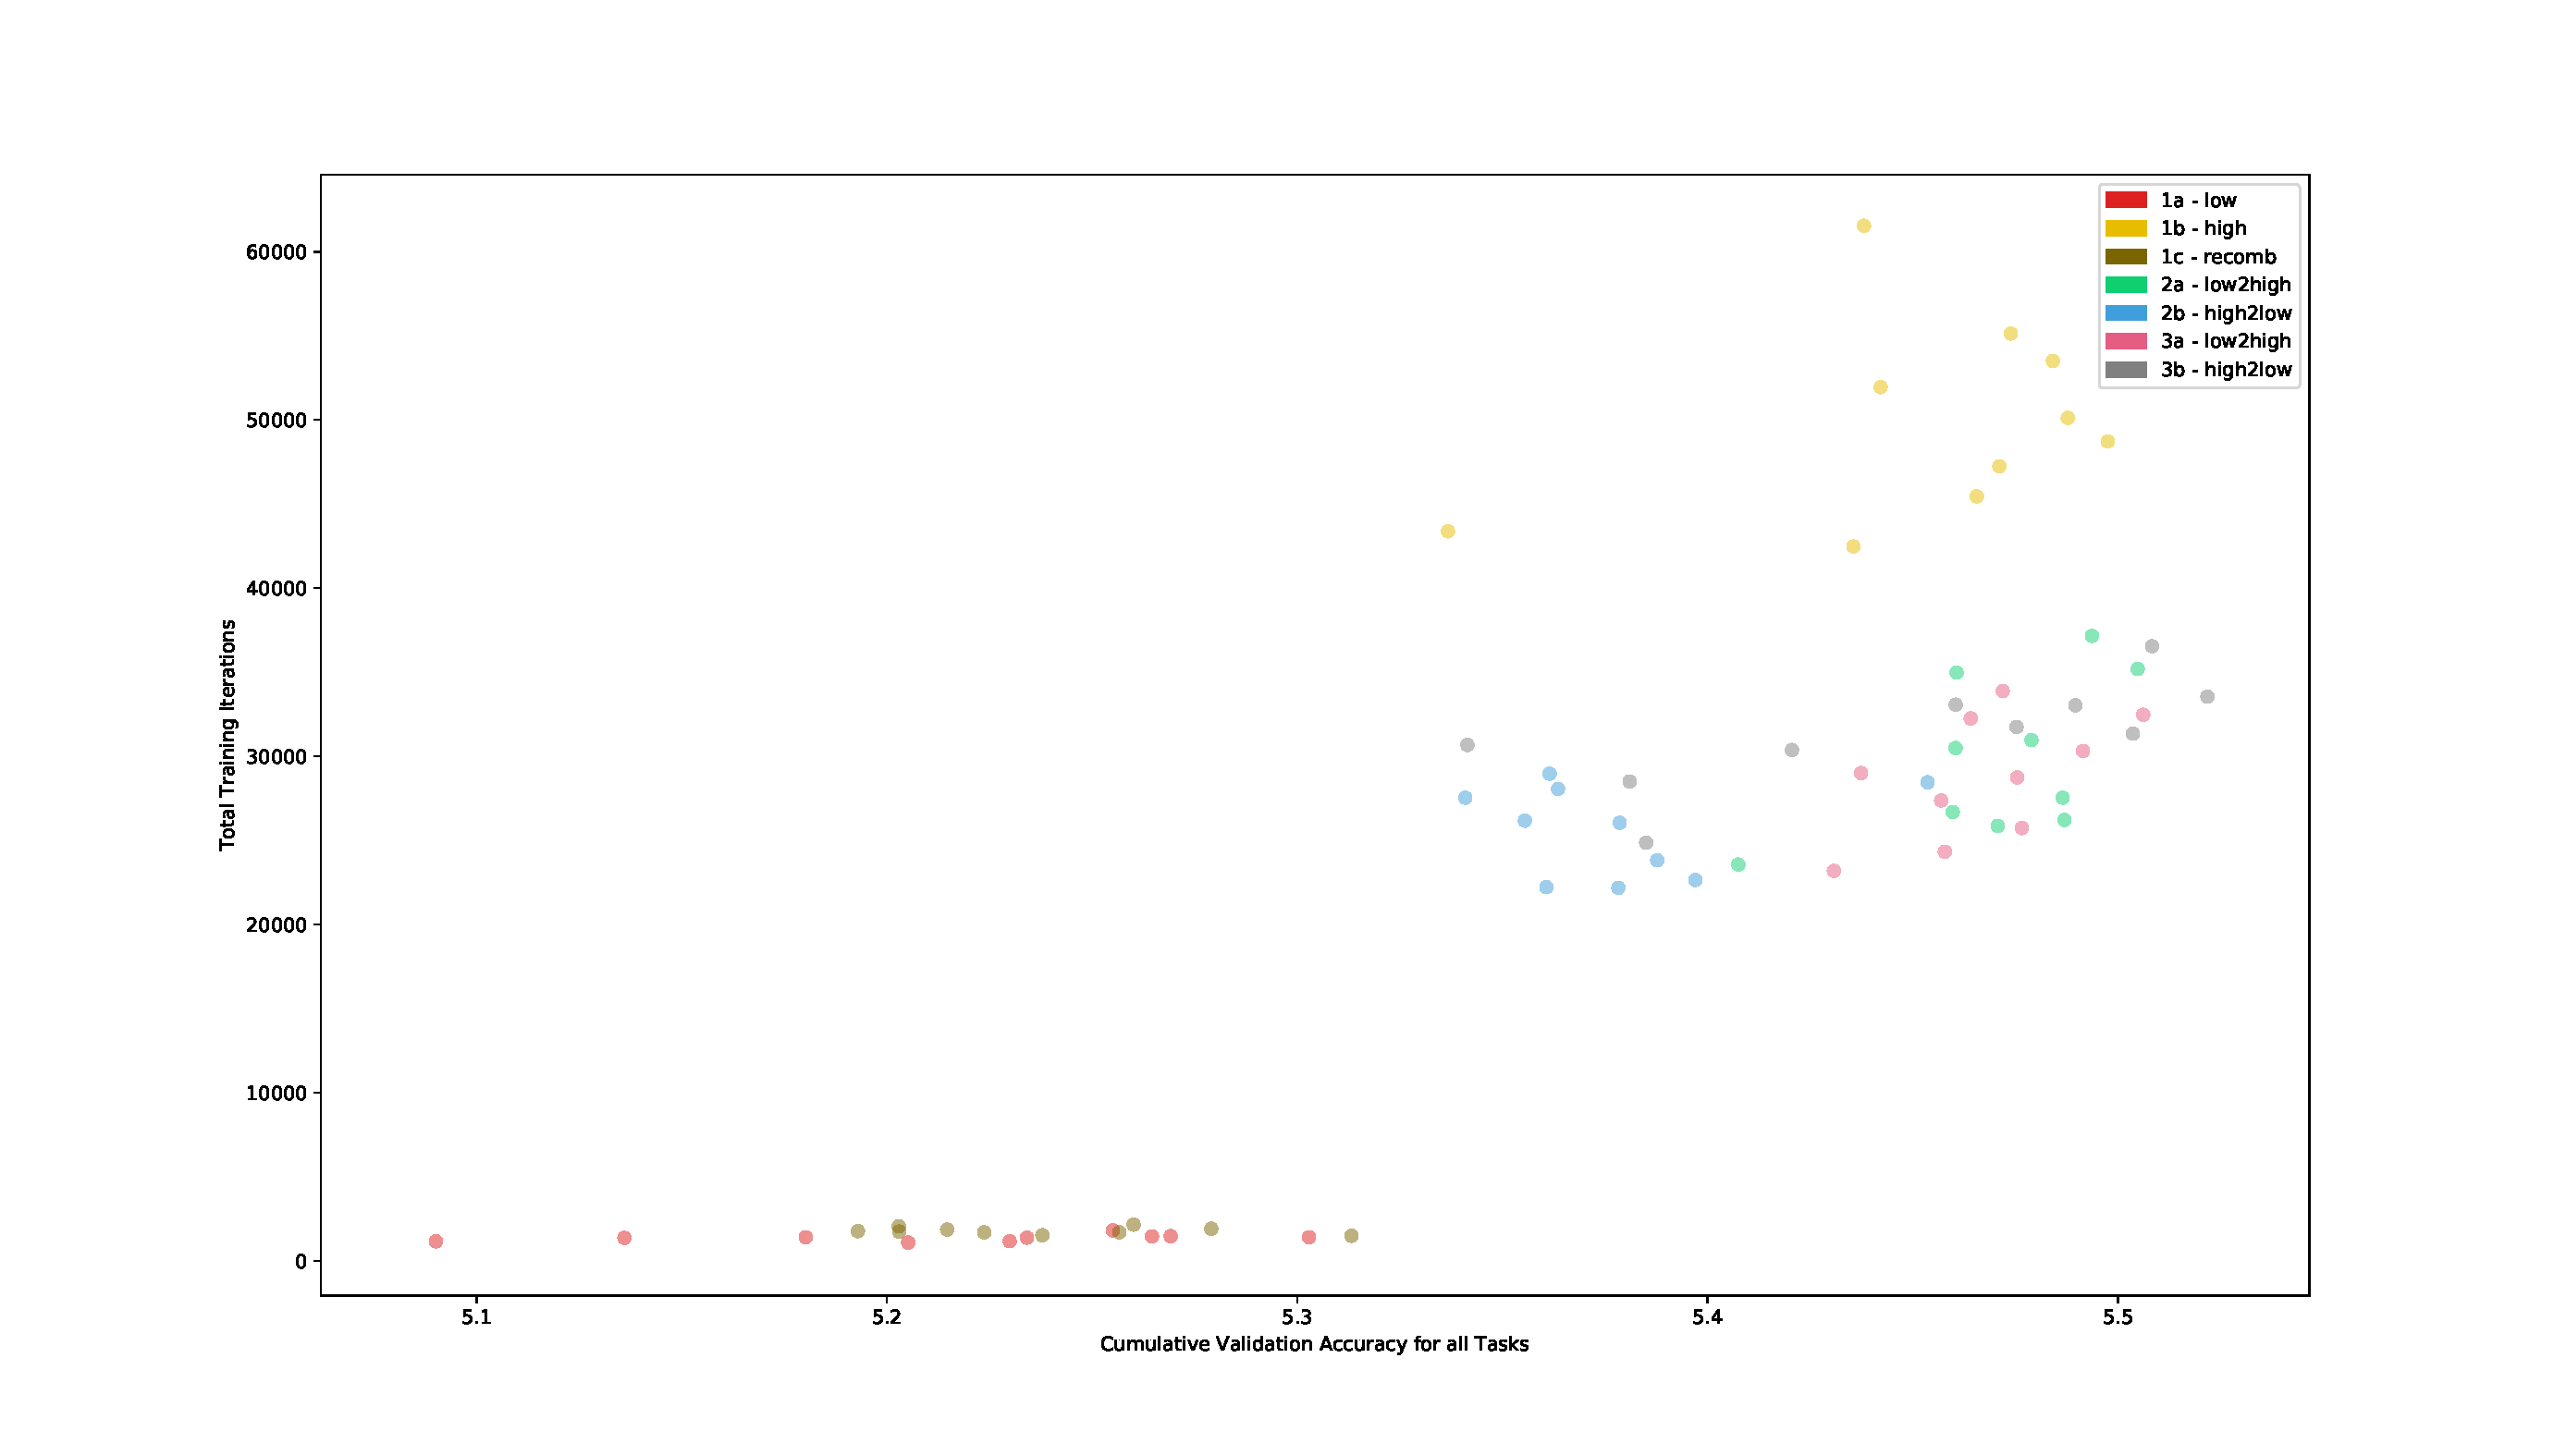
\includegraphics[width=1.2\textwidth,center]{Chapters/4.Experiments/exp2/figures/large/Training_value.pdf}
    \caption[Training vs cumulative accuracy plot]{The total amount of training in all optimal paths for each multi-task learning sequence plotted against the cumulative validation accuracy reached for that sequence. The circle size corresponds to the total number of used PathNet modules.}
    \label{fig:search.training_value}
\end{sidewaysfigure}

Training value figure \ref{fig:search.training_value} shows us much of the same as \ref{fig:search.validation}, the difference being the x-axis is the cumulative accuracy reached for all six tasks and the y-axis shows the total amount of training units for all optimal paths found. The circle radius for each trial is correlated to the total use of modules. 

The similarity in performance for algorithms 1a and 1c is present here also, as well as the similarity in validation accuracy for algorithms 1b, 2a, 2b, 3a and 3b. These are separated in training amount, however, which is not surprising as this is highly correlated to the tournament size and this changes between the algorithms. The difference in cumulative accuracy between task 2a and 2b seem to be about 0.1, and can therefore be explained by solely by the difference in validation accuracy between these two algorithms for task 4 as seen in figure \ref{fig:search.validation}. The small tournament size of 2 in algorithms 2b is yields a accuracy around 10 percentage points lower than 2a for this task, giving 2b a lower cumulative score in figure \ref{fig:search.training_value}. Tournament size 2 is still enough to reach a high performance for task 1a, which means this inequality is not equalized when 2a use a low tournament size. 

MWW testing of training amounts does not introduce something not found in plot \ref{fig:search.training_value}. Algorithms 1a, 1b and 1c are significantly different from all other algorithms, including each other. Within the cluster of algorithms 2a, 2b, 3a and 3b, the only pair that differ is 2a and 3b. 

\subsection{Discussion}
For the three first tasks 1a, 1b and 2 (all based on MNIST) figure \ref{fig:search.accuracy} the tasks are too simple for the algorithms to show any difference as any selection pressure used are capable of reaching a high performance for these tasks. For those based on cSVHN however, a clear split is visible for the algorithms. The split seem to follow the same pattern as the diversity plots \ref{fig:search.hamming_diversity} and \ref{fig:search.frequency_diversity_unique}. The low selection pressure algorithms are steadily increasing in fitness throughout the search and the fitness is still improving when the search terminates, hinting at 100 generations being to little for these algorithms to reach the same performance as those of higher tournament sizes. This is what was hypothesized and is explained by the increase in evaluations (and therefore also training units) for algorithms with higher tournament sizes. The similar fitness progression of 2a and 2b when using tournament size of 10 and higher to that of algorithms 1b, 3a and 3b is interesting however. This points towards performance of tournament size above 10 not being different. Figure \ref{fig:search.validation} supports this suspicions. The ANOVA tests for these results are indeed statistically significant.

When setting this accuracy in context of training in figure \ref{fig:search.training_value} it becomes clear the maximum tournament size of 25 is set unnecessarily high. A static use of tournament size around 10 would yield a similar accuracy performance to that of algorithms 1b, 2a, 2b, 3a and 3b while having a significantly lower training amount than any of these.

\section{Tournament size range}

For these experiments the results show that using a tournament size above 10 is unnecessary. Under this assumption, algorithms 3a and 3b would more than likely perform differently as their increase in selection pressure were intended to be more or less linear, while it here reaches the top level of selection pressure within the first 40\% of each search. 

As the plot \ref{fig:search.accuracy} show, the algorithms with high tournament size reach their maximum fitness quite early in the search. The remaining 60\% of search time\footnote{During the last 60\% of the search, algorithm 3a have functionally the maximum amount of selection pressure. This is also the case for algorithm 3b for the \textit{first} 60\% of the search} should be enough search time to learn each task. I.e: algorithms 3a and 3b effectively function the same as algorithm 1b.

By changing the range of tournament size these algorithms use would presumably reduce their accuracy performance to be somewhere between that of constantly high and constantly low selection pressure.

To verify the change in selection pressure have a effective range from the low tournament size in algorithms 1a and 1c and to tournament size 10, algorithms 3a and 3b are run again within the range \([2,\dots,10]\). MWW tests provided the results found in table \ref{tab:exp2.dynamic_rerun}, where algorithm 3a with the range 2 through 25 is compared to algorithm 3a with range 2 through 10, and the same comparison made for algorithm 3b. 

\begin{table}[h]
    \centering
    \begin{tabular}{lrrrrrr}
            & \multicolumn{2}{r}{Reuse} & \multicolumn{2}{r}{Accuracy} & \multicolumn{2}{r}{Path size} \\
            & 3a          & 3b          & 3a            & 3b           & 3a            & 3b            \\
    Task 1a &             &             & 0.6771        & 0.0279       & 0.9690        & 0.5593        \\
    Task 1b & 0.9565      & 0.9565      & 0.9397        & 0.4488       & 0.1816        & 0.2366        \\
    Task 2  & 0.5381      & 0.5621      & 0.5966        & 0.6775       & 0.8770        & 0.2440        \\
    Task 3a & 0.6028      & 1.0         & 0.8205        & 0.4272       & 1.0           & 0.8770        \\
    Task 3b & 0.7576      & 0.6969      & 0.6224        & 0.0815       & 0.9057        & 0.0624        \\
    Task 4  & 0.2687      & 0.7837      & 0.0539        & 0.6500       & 0.1361        & 0.3086       
    \end{tabular}
    \caption{P-values from comparing algorithms 3a and 3b for a tournament size range of \([2,\dots,25]\) with range \([2,\dots,10]\). \(\alpha=1.57\times 10^{-3}\)}
    \label{tab:exp2.dynamic_rerun}
\end{table}

While there is an obvious difference in training units because of the reduced number of evaluations during each search, there is no significant difference in any other tested metrics. Confirming that this case of multi-task problems and PathNet structure, the effective range of tournament sizes spans from the minimum 1\footnote{Tournament size 1 is the same as performing a stochastic search} to 10.

\section{Conclusion}

The choice of only turning the tournament size dial in these experiments were a conscious one. Parameters such as search termination limit, population size, task-set might lead to other results than those observer here, so ultimately the conclusions drawn are limited by the hyper-parameter space explored. 

Continuation to these experiments should include trials where harder tasks from a more varied domain spectrum are explored. This would encourage using a larger PathNet structure and by increasing the number of allowed module permutations, the search-space increase greatly which again would call for an increase in population size. All these changes brings with it a considerable increase in computational requirements however.

Answering the questions raise in the introduction to this chapter proved to be tougher than originally thought as these experiments only seem to scratch the surface of GA's as optimizer for a Super Neural Network. These results show however, that limiting the tournament size to around 10 can be done for a population size of 64 without taking a hit on performance. Also shown is that tuning the tournament size does shift the search from exploration to exploitation. If this shift affect the search in any significant way should be tested with a harder task-set than used here. 

These experiments also confirm the difficulty in measuring population diversity without misrepresentations. For debugging and testing search parameters, a combination of pair-wise Hamming distance and a frequency count seem to provide a fair balance between favouring identical genomes and genetic similarities.  


\chapter{Experiment 3: Relearning a task}
\label{exp3}
The motivation behind reusing modules is as mentioned in the introduction, to increase the number of tasks a PathNet can learn before being saturated by decreasing the amount of new capacity a path needs for a new task. A optimal search algorithm for new paths should therefore be able to reuse as much knowledge as possible without limiting the performance. If we assume a ideal search algorithm would find optimal modules for each task, it should be able to find and reuse all learned knowledge if a task is learned twice. 

We can put this to a test by learning some task twice for all seven algorithms in chapter \ref{exp2}. As the amount of module reuse in these experiments were small, we lower the proverbial bar here by reducing the module search space.

The question we want to answer is this: \textit{"Given optimal conditions for module reuse\footnote{By optimal conditions we mean learning the same task twice in a small PathNet structure.}, which selection pressure scheme is best suited for knowledge reuse?"}

\section{Description}
The experimental structure here is simple. The same experimental parameters as the experiment in chapter \ref{exp2} are used again, but here the the seven algorithms will here be applied to a binary task problem where both tasks are the same: a cSVHN classification problem with all 10 classes. After searching for a optimal path for both tasks, the reuse is noted. 

By performing this experimental trial for each algorithm multiple times, we can compare the observations of reuse with the probability of seeing these results in random path selection, and then with each other. 

\section{Hypothesis}
Based on the reuse in the previous selection pressure experiments, we do not expect any algorithm to yield perfect results\footnote{Perfect results here would constitute finding all modules used in the previous path}, but have a statistically significant difference from random path selection. Given the algorithms different selection pressures, they are expected to give somewhat different reuse results and I would expect the higher exploration algorithms to yield more reuse, as the amount of parameter optimization needed to give high fitness is relatively small. The advantage the high tournament size algorithms (algorithm 1b and to some degree 2a, 2b, 3a and 3b) have by evaluating more paths should be reduced, as these algorithms have a higher selection pressure and converge quicker. 

\section{Implementation}
The experiment structure here is a binary task problem, where we want to find two paths for a full cSVHN classification problem twice, meaning both task 1 and task 2 is cSVHN classification with all classes. The two searches should have a non-zero probability of reusing no modules, so the PathNet dimensions are set to 3 layers of 6 modules each with a maximum of 3 active modules pr. paths layer. We can describe the total number of possible paths as 
\begin{equation*}
    \prod_{i=0}^{\omega-1}(M-i)^{L}
\end{equation*}
where \(\omega\) is the maximum number of active modules in each layer for each path, \(M\) is the number of modules in each PathNet layer and  \(L\) is the number of layers in the PathNet. This means the number of possible paths in a 20-by-3 PathNet with \(\omega=3\) is  
\begin{equation*}
    \prod_{i=0}^{3-1}(20-i)^{3}\approx 3.2\times10^{11}
\end{equation*}
and in this experiment
\begin{equation*}
    \prod_{i=0}^{3-1}(6-i)^{3}\approx 1.7\times10^{6}
\end{equation*}
Reducing the PathNet size from 20 modules in each layer to 6 have reduced the search space with 5 orders of magnitude, and it should therefore be significantly easier to find reusable modules here than in the previous experiment.

We can approximate the probability of finding any number of reuse by randomly selecting two paths within the limitations of the PathNet dimensions and path-size with a Monte-Carlo approach. Using equation \ref{eq:montecarloP} where we want the probabilities to be minimum 10 times as large as the standard deviation (\(R=0.1\)) and \(n=10^{9}\) Monte-Carlo trials, we calculate the probability accuracy to be 
\begin{equation*}
    \frac{1}{nR^{2}+1}=\frac{1}{10^{7}+1}\approx10^{-7}
\end{equation*}
Meaning we can tell the probability of reuse to the seventh decimal place from the Monte-Carlo results. The results of the performed Monte-Carlo estimation can be found in table \ref{tab:montecarlo}.

\begin{table}[ht]
    \centering
    \begin{tabular}{clll}
    \# of reuse & \# of outcomes & Monte-Carlo probabilities & Rounded  \\
    0           & 88892859      & 0,088892859               & 0,0888928 \(\pm 10^{-7}\)  \\
    1           & 266671854     & 0,266671854               & 0,2666718 \(\pm 10^{-7}\)  \\
    2           & 327560805     & 0,327560805               & 0,3275608                  \\
    3           & 213925123     & 0,213925123               & 0,2139251                  \\
    4           & 81393230      & 0,08139323                & 0,0813932                  \\
    5           & 18720470      & 0,01872047                & 0,0187205                  \\
    6           & 2612531       & 0,002612531               & 0,0026125                  \\
    7           & 213747        & 0,000213747               & 0,0002137 \(\pm 10^{-7}\)  \\
    8           & 9195          & 0,000009195               & 0,0000092                  \\
    9           & 186           & 0,000000186               & 0,0000002                 
    \end{tabular}
    \caption{Results from Monte-Carlo approximation of reuse probabilities for two paths in a 6-by-3 PathNet with a maximum of 3 active modules in each layer.}
    \label{tab:montecarlo}
\end{table}

For comparison to the experimental results, we will calculate the expected reuse for the number of experimental trial run, and compare the mean reuse value to the mean reuse of each algorithm. The means will be compared through ANOVA tests with a significance level of 0.05  
\section{Results}
\section{Discussion}
\section{Conclusion}

\chapter{Thesis Conclusion}

\section{Experimentation summary}
\subsection{Experiment 1: Selection versus search}
The first results using binary MNIST tasks turned out to be too simple. When the task difficulty was increased, and the module structure changed from fully connected neurons to convolutional operations, both searches cause the same amount of training in the selected path. This uncovered that the end-to-end training of the first path caused less reuse than when the first path was found by searching. As the search termination here was a threshold accuracy, the equal training amount of both end-to-end training and full path search tells us the problems with end-to-end training in a modular structure lies in the modules transferability, and not accuracy performance.

\subsection{Experiment 2: Selection pressure}
The different selection pressures influenced training predictably. The increase in tournament size, and therefore also the number of evaluations per generation, yielded more training, quicker convergence to a path, and each generation provided a larger increase in fitness. No difference in reuse was found, and all algorithms reused less than would have been done if all modules were selected randomly. 

\subsection{Experiment 3: Relearning a task}
Training under ideal reuse conditions did cause more reuse than by random module selection for all algorithms. However, there were only minor differences between the algorithms and no distinct patterns in reuse among the different training amounts or tournament sizes. 

The availability of trained modules to reuse caused a more rapid increase in fitness for the first generations for the second task than the first.  

\section{Discussion}
As experienced in chapter \ref{exp1}, the selected problems domain-complexity has a large influence on how the PathNet behaves during training. The advantage to module reuse and modular training was not as prominent as expected. However, there are some claims that can be made to some degree of certainty.

\begin{itemize}
    \item \emph{The transferability of modules is effected by the context in which the modules are trained}
\end{itemize}
The experiments in chapter \ref{exp1} provided evidence for this by concluding to end-to-end training causing more parameters less well suited for module reuse. This insight colored the expectation for results in chapter \ref{exp2} and \ref{exp3}. The expectations based on chapter \ref{exp1} was that modules trained as part of multiple paths would have a higher likelihood of being reused. Larger tournament sizes was hypothesized to provide a higher selection pressure than small tournament sizes, and end-to-end training could be classified as having the highest possible selection pressure. Therefore, the lower tournament size algorithms (mainly 1a and 1c) were expected to have a higher level of module reuse than the rest of the algorithms. Neither the results in chapter \ref{exp2}, nor chapter \ref{exp3} show evidence for this being the case. Further experimentation is needed to uncover if this holds true for a more complex task domain. 

During the experimentation in chapter \ref{exp2} the results for diversity and validation accuracy yielded another insight: 
\begin{itemize}
    \item \emph{There is a diminishing return in the exploitation of a search when increasing the tournament size}
\end{itemize}
This motivated another set of experimental trials for algorithms 3a and 3b as the tournament sizes above 10 having a comparable convergence. Mann-Whitney testing the difference between this new maximum tournament size and the old one of 25 for both algorithms confirmed that there was no significant difference.

When performing the last experiments in chapter \ref{exp3}, this new maximum tournament size was used for all algorithms utilizing a high tournament size. The ideal circumstances gave an overall higher module reuse level than the preceding experiment, but the different selection pressures did not perform significantly different from each other. However, confirmation of PathNet's merits was found in this chapter. 

\begin{itemize}
    \item \emph{Higher reuse of modules when the source and target task domain is similar yield quicker training.}
\end{itemize}
While this is merely a validation of the results DeepMind found in \cite{pathnet}, the results for module reuse hint at the task domain being too simple which makes the performance increase from reusing modules surprising. 

Reaching results from which we can draw strongly supported insights about whether exploration does provide better transferability of knowledge requires these experiments to be tested with more complex tasks. We can assume that demanding more from the network structure regarding capacity would require a larger PathNet structure and adjustments made to the search termination limits. In such a case, each evaluation would provide a smaller fitness increase, and more focus might be placed on finding better parameters currently in the PathNet-state. 

\section{Future work}
This thesis lay foundations which need to be built on to reach a more in-depth understanding of transferability of parameters in a modular context. During the work, multiple unanswered questions appeared which is presented here as possible future work. 

\subsection{More complex task-domain}
As mentioned, the behavior of high exploration and high exploitation search algorithms might be different when using a more complex task-set. For binary MNIST classification in chapter \ref{exp1}, the expected decrease in reuse for end-to-end training was not present due to the task-domain being too simple. This might also be the reason why none of the algorithms used in chapter \ref{exp2} or \ref{exp3} caused different levels of reuse. For instance, training paths to provide reinforcement signals for different locomotion tasks provides an intuitive divide between problems as the different tasks could be different environments through which the agent moves.   

\subsection{Module optimization with other search algorithms}
The use of tournament search for optimal module selection only scratches the surface of possible algorithm choices. The use of evolutionary search methods might provide a better exploration of module permutation-space, and cause different effects on performance. 

\subsection{Saturating a PathNet}
As PathNet by design is restricted in the number of parameters, at some point, all modules are locked to backpropagation. Each subsequent problem applied to the structure would consist of only reused modules, and the only parameter optimization would be that of the task-unique final layer. Such a saturated PathNet structure might lead to a high abstraction level output from the final module layer, and new tasks could be learned using little training data and only a small amount of new capacity. 

It would be necessary for such a scenario too, device a proficient search algorithm which both provides good module choices during the saturation process and good choices after new modules are unable to be trained. 

\subsection{Convergence increase when reusing modules}
The reason behind algorithm 1c's increased convergence for task 2 in chapter \ref{exp3} is not understood. The experiment should be replicated to check if the result is consistent, and investigating the reason behind this effect. 



\iffalse
Future work on the topics in this thesis should include such an increase in task difficulty and module structure. As these experiments only start to explore the possibilities in genetic algorithms for path optimization, multiple possible techniques could be used. In the name of minimizing the amount of capacity used for each task through module reuse, exploring the properties of a saturated PathNet might prove interesting. As the amount of open and available untrained parameters diminish, the importance of effective and appropriate path-optimization would surpass the significance of parameter optimization. 

While the object-oriented implementation of PathNet and its path search worked well in these experiments, an increase in computational requirements would justify the effort of creating a GPU implementation of the search algorithm. 



- How did we interpret the results?
- What did we learn?
- What questions did we answer?
- did we answer all original research questions?

- What did we not answer? 
* Why did we not?
* How could this be answered?

\section{Future works}
- How did this implementation work?
* what worked well?
* What could be better?

- Which experiments would be a natrual continuation of this work?
* What would they answer?
* why are these different from what I did?




Are your results satisfactory? 
Can they be improved? 
Is there a need for improvement? 
Are other approaches worth trying out? 
Will some restriction be lifted? 
Will you save the world with your Nifty Gadget? 

\section{Discussion} 
Discussion of the accuracy and relevance of the results; comparison with other researchers results. 
\subsection{Common errors}
Too far reaching conclusions; guesswork not supported by the data; introduction of a new problem and a discussion around this.  

\section{Conclusion} 
Consequences of the achieved results, for example for new research, theory and applications. 

\subsection{Common errors}
The conclusions are too far reaching with respect to the achieved results; the conclusions do not correspond with the purpose
\fi


\newpage
\emergencystretch=2em
\printbibliography

\begin{appendices}
    \chapter{Pair-wise Hamming reduction}
\label{appendix:Hammingreduction}
The main problem with Hamming distance as a metric is that the number of computations needed is quadratic with the population size P. Meaning the computational time is quite long for large populations. In the context of the variable selection pressure experiments, this metric is calculated 42000 times\footnote{Once every generation through all path optimizations for all tasks which are 600. This is then done for every experimental run of every algorithm (70 times)}.

\section{Moment of Inertia}
Morrison et al. presented\cite{populationDiversity} an alternative diversity metric which they proved to yield the same results as pair-wise Hamming, but was calculable in linear time with respect to P. Their solution was based on the concept of moment of inertia for measurement of mass distribution into arbitrarily high dimensionality space, where a centroid genome C was calculated for the population of genomes, where the i-th element of that centroid is
\begin{equation}
    \label{eq:centroid}
    C_{i}=\tfrac{1}{P}\sum_{j=1}^{P}y_{ji}
\end{equation}
and the moment of inertia I is given as 
\begin{equation}
    \label{eq:Inertiadiversity}
    I  = \sum_{i=1}^{L}\sum_{j=1}^{P}\left ( y_{ij}-C_{i} \right )^{2}
\end{equation}
They then prove \(PI\) = pair-wise Hamming distance.

Introduced here is a reduction of the pair-wise Hamming formula from having a quadratic computation time with respect to P to a linear computation time under the assumption of a binary genome. This method does not improve on the centroid moment of inertia method with the same leap in computation time as from quadratic to linear time, but the algorithm derived from this formula is proved to be quicker. 

\section{Reduction}
First, the problem is reduced to a genome length L = 1 and index \({j}'\) is renamed to i for readability.
\begin{equation*}
    H_{1}=\sum_{j=1}^{P-1}\sum_{i=j+1}^{P}\left |y_{j}-y_{i}\right |
\end{equation*}
Because of the absolute-value, \(\left |y_{j}-y_{i}\right |\) equals \(\left |y_{i}-y_{j}\right |\), which means the nested summations can be rewritten\footnote{This is best visualized as the area of a matrix these sums cover. The sums where both i and j goes from 1 to P would cover the whole matrix, while the original \(H_{1}\) cover a triangle in one of the matrix corners with the last sum in equation \ref{eq:hammingreductionsums} covering the diagonal of the matrix.} so that both span the whole population length, P.
\begin{equation}
    \label{eq:hammingreductionsums}
    \sum_{j=1}^{P}\sum_{i=1}^{P}\left | y_{j}-y_{i} \right | = 2\left [ \sum_{j=1}^{P-1}\sum_{i=j+1}^{P}\left | y_{j}-y_{i} \right | \right ]+ \sum_{i=1}^{P}\left | y_{i}-y_{i} \right | 
\end{equation}
The last sum in equation \ref{eq:hammingreductionsums} evaluates to zero, which means we can express \(H_{1}\) as 
\begin{equation*}
    H_{1} = \frac{1}{2}\sum_{j=1}^{P}\sum_{i=1}^{P}\left | y_{j}-y_{i} \right |
\end{equation*}
By isolating the inner summation in the new expression for \(H_{1}\) we can hold \(y_{j}\) constant to either 0 or 1, since \(y_{i}\in\left [0, 1\right]\) for all i. When \(y_{j}=0\), the inner sum evaluates to the number of 1's in our set of y's. In the cases of \(y_{j}=1\), the inner sum evaluates to the number of 0's. This is the pair-wise Hamming formula counting the inequalities in the genome within pairs in the population.

Since \(y_{i}\in\left [0, 1\right]\), we can express counting the occurrences of 0's and 1's as
\begin{equation*}
    \textnormal{Number of 1's in population} = \sum_{j=1}^{P}y_{j} 
\end{equation*}
\begin{equation*}
    \textnormal{Number of 0's in population} = P-\sum_{j=1}^{P}y_{j}
\end{equation*}

At this point, it becomes clear that what the two sums do is summing the number of ones for every zero in the population plus the number of 0's for every 1. Which means we again can rewrite \(H_{1}\). 

\begin{equation*}
    H_{1} = \frac{1}{2}\left [\sum_{j=1}^{P}y_{j}\left (P - \sum_{j=1}^{P}y_{j} \right) + \left (P - \sum_{j=1}^{P}y_{j} \right)\sum_{j=1}^{P}y_{j}\right ]
\end{equation*}

\begin{equation}
    \label{eq:linearHamming}
    H_{1} = \sum_{j=1}^{P}y_{j}\left (P - \sum_{j=1}^{P}y_{j} \right)
\end{equation}

The generalization from a one-dimensional genome to L dimensions is trivial because when counting pairwise genome differences, the same result is reached whether counting a pair-wise Hamming for each genome separately and then adding them together, or the total Hamming distance is counter for all genes first. Ergo, for a population of size P of binary genomes of length L
\begin{equation}
    \label{eq:proved}
    \sum_{j=1}^{j=P-1}\sum_{{j}'=j+1}^{{j}'=P}\sum_{i=1}^{i=L}\left |y_{ij}-y_{i{j}'}\right | = \sum_{i=1}^{L}\sum_{j=1}^{P}y_{j}\left (P - \sum_{{j}'=1}^{P}y_{{j}'} \right)
\end{equation}

This version of the Hamming distance can be calculated in 2LP which is a small improvement on the centroid moment of inertia method which performed in \(4LP + L\) calculations. 



    \chapter{Mann-Whitney p-tables}

\section{Capacity usage}
\label{appendix:ptable.capacity}
\begin{table}[h!]
    \centering
    \begin{tabular}{cccccccc}
                  & \textbf{1a}  & \textbf{1b}  & \textbf{1c}  & \textbf{2a}  & \textbf{2b}  & \textbf{3a}  & \textbf{3b}  \\
    \textbf{1b}   & 0.4222505332 &              &              &              &              &              &              \\
    \textbf{1c}   & 0.2855293965 & 0.6174309237 &              &              &              &              &              \\
    \textbf{2a}   & 0.7280652457 & 1.0000000000 & 0.7897870595 &              &              &              &              \\
    \textbf{2b}   & 0.8477118512 & 0.4012174952 & 0.2220797830 & 0.6752726661 &              &              &              \\
    \textbf{3a}   & 0.9387465832 & 0.4460788518 & 0.2701356925 & 0.4925264269 & 0.9090383245 &              &              \\
    \textbf{3b}   & 0.5640824263 & 0.7029987613 & 0.8791509539 & 0.9389357051 & 0.5424518014 & 0.4925264269 &              \\
    \textbf{Rand} & 0.0000589269 & 0.0013875064 & 0.0013875064 & 0.0000615822 & 0.0014074877 & 0.0014074877 & 0.0013808872
    \end{tabular}
    \caption[p-table for capacity use]{Two-sided p-values for the distribution of module use. \(\alpha\) value 0.00179}
    \label{tab:exp2.capacityptable}
\end{table}


\section{Module reuse}
\label{appendix:ptable.reuse}
\begin{table}[h!]
    \centering
    \begin{tabular}{cccccccc}
                              & \textbf{1a} & \textbf{1b} & \textbf{1c}  & \textbf{2a} & \textbf{2b} & \textbf{3a} & \textbf{3b} \\
    \textbf{1b}               & 0.39684 &         &         &         &         &         &         \\
    \textbf{1c}               & 0.51591 & 0.09509 &         &         &         &         &         \\
    \textbf{2a}               & 0.08803 & 0.34808 & 0.01494 &         &         &         &         \\
    \textbf{2b}               & 1.00000 & 0.28050 & 0.58683 & 0.06483 &         &         &         \\
    \textbf{3a}               & 0.12563 & 0.55323 & 0.02487 & 0.74871 & 0.09667 &         &         \\
    \textbf{3b}               & 0.84754 & 0.56589 & 0.53840 & 0.19366 & 0.96949 & 0.25069 &         \\
    \textbf{Rand}             & 0.00137 & 0.00136 & 0.11354 & 0.00006 & 0.01695 & 0.00005 & 0.00138
    \end{tabular}
    \caption[Experiment 2: p-table for module reuse]{Two-sided p-values for the distribution of module reuse.\(\alpha\) value 0.00179}
    \label{tab:exp2.reuseptable}
\end{table}

\newpage
\section{Total training used}
\label{appendix:ptable.training}
\begin{table}[h!]
    \centering
    \begin{tabular}{cccccccc}
                & \textbf{1a}  & \textbf{1b}  & \textbf{1c}  & \textbf{2a}        & \textbf{2b}        & \textbf{3a}       \\
    \textbf{1b} & 0.00018 &         &         &         &         &         \\
    \textbf{1c} & 0.00101 & 0.00018 &         &         &         &         \\
    \textbf{2a} & 0.00018 & 0.00018 & 0.00018 &         &         &         \\
    \textbf{2b} & 0.00018 & 0.00018 & 0.00018 & 0.05869 &         &         \\
    \textbf{3a} & 0.00018 & 0.00018 & 0.00018 & 0.57075 & 0.05390 &         \\
    \textbf{3b} & 0.00018 & 0.00018 & 0.00018 & 0.42736 & 0.00131 & 0.12122
    \end{tabular}
    \caption[Experiment 2: p-table for training units]{Two-sided p-values for the distribution of training units. \(\alpha\) value 0.00238}
    \label{tab:exp2.trainingptable}
\end{table}

\begin{table}[h!]
    \centering
    \begin{tabular}{cccccccc}
                              & \textbf{1a}        & \textbf{1b}        & \textbf{1c}        & \textbf{2a}        & \textbf{2b}  & \textbf{3a}  \\
    \textbf{1b}               & 0.0008380018       &                    &                    &                    &              &              \\
    \textbf{1c}               & 0.5198945164       & 0.0003097918       &                    &                    &              &              \\
    \textbf{2a}               & 0.5447441365       & 0.0001697296       & 0.9393549041       &                    &              &              \\
    \textbf{2b}               & 0.0005016186       & 0.7900997653       & 0.0002421738       &  0.0001786145      &              &              \\
    \textbf{3a}               & 0.0004942973       & 0.1835533262       & 0.0002041395       &  0.0001756155      & 0.1847169358 &              \\
    \textbf{3b}               & 0.0072406695       & 0.2521504314       & 0.0007545410       &  0.0003213758      & 0.4035495809 & 0.0634225474 
    \end{tabular}
    \caption[p-table for validation accuracy (task 1a)]{Two-sided p-values for the distribution of validation accuracy scores for task 1a. \(\alpha\) value 0.00238}
    \label{tab:exp2.validation1a}
\end{table}

\begin{table}[h!]
    \centering
    \begin{tabular}{ccccccc}
                & \textbf{1a}        & \textbf{1b}        & \textbf{1c}        & \textbf{2a}  & \textbf{2b}  & \textbf{3a}  \\
    \textbf{1b} & 0.0009991495       &                    &                    &              &              &              \\
    \textbf{1c} & 0.9094843977       & 0.0001806347       &                    &              &              &              \\
    \textbf{2a} & 0.0019245079       & 0.4721755506       & 0.0003230557       &              &              &              \\
    \textbf{2b} & 0.0004352788       & 0.5202090058       & 0.0001806347       & 0.1498505300 &              &              \\
    \textbf{3a} & 0.0007615180       & 0.5697331203       & 0.0001806347       & 0.2261266965 & 0.7051398030 &              \\
    \textbf{3b} & 0.0045254314       & 0.4958052761       & 0.0007615180       & 0.8499394098 & 0.1847169358 & 0.3839570356
    \end{tabular}
    \caption[p-table for validation accuracy (task 1b)]{Two-sided p-values for the distribution of validation accuracy scores for task 1b. \(\alpha\) value 0.00238}
    \label{tab:exp2.validation1b}
\end{table}

\begin{table}[h!]
    \centering
    \begin{tabular}{ccccccc}
                & \textbf{1a}        & \textbf{1b}        & \textbf{1c}        & \textbf{2a}  & \textbf{2b}  & \textbf{3a}  \\
    \textbf{1b} & 0.0003281333 &                    &                    &              &              &              \\
    \textbf{1c} & 0.6774705128 & 0.0003298385       &                    &              &              &              \\
    \textbf{2a} & 0.0002434867 & 0.0960533908       & 0.0001816511       &              &              &              \\
    \textbf{2b} & 0.0001816511 & 0.1041098897       & 0.0001826718       & 0.8204630988 &              &              \\
    \textbf{3a} & 0.0001806347 & 0.1506196716       & 0.0001816511       & 0.7616726080 & 0.5706055035 &              \\
    \textbf{3b} & 0.0001816511 & 0.2730363398       & 0.0001826718       & 0.3844942826 & 0.3843153515 & 0.3844942826
    \end{tabular}
    \caption[p-table for validation accuracy (task 2)]{Two-sided p-values for the distribution of validation accuracy scores for task 2. \(\alpha\) value 0.00238}
    \label{tab:exp2.validation2}
\end{table}

\newpage

\begin{table}[h!]
    \centering
    \begin{tabular}{ccccccc}
                & \textbf{1a}        & \textbf{1b}        & \textbf{1c}        & \textbf{2a}  & \textbf{2b}  & \textbf{3a}  \\
    \textbf{1b} & 0.0004396388 &                    &                    &              &              &              \\
    \textbf{1c} & 0.7337299957 & 0.0004396388       &                    &              &              &              \\
    \textbf{2a} & 0.0001826718 & 0.0081270247       & 0.0001826718       &              &              &              \\
    \textbf{2b} & 0.0002448048 & 0.0450737863       & 0.0002448048       & 0.4053255516 &              &              \\
    \textbf{3a} & 0.0004396388 & 0.2730363398       & 0.0005828399       & 0.5205228833 & 0.9096880762 &              \\
    \textbf{3b} & 0.0003298385 & 0.1507733379       & 0.0002461281       & 0.2566603699 & 0.6230455308 & 0.9097218891
    \end{tabular}
    \caption[p-table for validation accuracy (task 3a)]{Two-sided p-values for the distribution of validation accuracy scores for task 3a. \(\alpha\) value 0.00238}
    \label{tab:exp2.validation3a}
\end{table}

\begin{table}[h!]
    \centering
    \begin{tabular}{ccccccc}
                & \textbf{1a}        & \textbf{1b}        & \textbf{1c}        & \textbf{2a}  & \textbf{2b}  & \textbf{3a}  \\
    \textbf{1b} & 0.0027962419       &                    &                    &              &              &              \\
    \textbf{1c} & 0.8500510249       & 0.0007615180       &                    &              &              &              \\
    \textbf{2a} & 0.0007650230       & 0.7051398030       & 0.0004396388       &              &              &              \\
    \textbf{2b} & 0.0408691075       & 0.1209446324       & 0.0113296967       & 0.0754416055 &              &              \\
    \textbf{3a} & 0.0057769786       & 0.4264846219       & 0.0017062494       & 0.1734555737 & 0.4495213258 &              \\
    \textbf{3b} & 0.0090303992       & 0.8497715188       & 0.0040303666       & 0.7335371872 & 0.2119499062 & 0.5700245022
    \end{tabular}
    \caption[p-table for validation accuracy (task 3b)]{Two-sided p-values for the distribution of validation accuracy scores for task 3b. \(\alpha\) value 0.00238}
    \label{tab:exp2.validation3b}
\end{table}

\begin{table}[h!]
    \centering
    \begin{tabular}{ccccccc}
                & \textbf{1a}        & \textbf{1b}        & \textbf{1c}        & \textbf{2a}        & \textbf{2b}        & \textbf{3a}  \\
    \textbf{1b} & 0.0005828399       &                    &                    &                    &                    &              \\
    \textbf{1c} & 0.1858767324       & 0.0017062494       &                    &                    &                    &              \\
    \textbf{2a} & 0.0001826718       & 0.6775849580       & 0.0001826718       &                    &                    &              \\
    \textbf{2b} & 0.7913367801       & 0.0004396388       & 0.0451545696       & 0.0001826718       &                    &              \\
    \textbf{3a} & 0.0001826718       & 0.9397203669       & 0.0002461281       & 0.6231762239       & 0.0002461281       &              \\
    \textbf{3b} & 0.0028272721       & 0.8205295061       & 0.0072845570       & 0.4726755935       & 0.0028272721       & 0.9698499770
    \end{tabular}
    \caption[p-table for validation accuracy (task 4)]{Two-sided p-values for the distribution of validation accuracy scores for task 4. \(\alpha\) value 0.00238}
    \label{tab:exp2.validation4}
\end{table}

\newpage


\begin{table}[h!]
    \centering
    \begin{tabular}{ccccccc}
                & \textbf{1a}  & \textbf{1b}  & \textbf{1c}  & \textbf{2a}  & \textbf{2b}  & \textbf{3a}  \\
    \textbf{1b} & 0.63400 &         &         &         &         &         \\
    \textbf{1c} & 0.63553 & 0.48508 &         &         &         &         \\
    \textbf{2a} & 0.17338 & 0.46322 & 0.18322 &         &         &         \\
    \textbf{2b} & 0.78408 & 1.00000 & 0.61495 & 0.54926 &         &         \\
    \textbf{3a} & 1.00000 & 0.78559 & 0.93856 & 0.44925 & 0.78658 &         \\
    \textbf{3b} & 0.90748 & 0.93750 & 0.93863 & 0.62691 & 0.84575 & 1.00000
    \end{tabular}
    \caption[Experiment 2: p-table for path sizes (task 1a)]{Two-sided p-values for the distribution of optimal path sizes for task 1a. \(\alpha\) value 0.00238}
    \label{tab:exp2.pathsize1a}
\end{table}

\begin{table}[h!]
    \centering
    \begin{tabular}{ccccccc}
                & \textbf{1a}  & \textbf{1b}  & \textbf{1c}  & \textbf{2a}  & \textbf{2b}  & \textbf{3a}  \\
    \textbf{1b} & 0.23894 &         &         &         &         &         \\
    \textbf{1c} & 0.01581 & 0.19860 &         &         &         &         \\
    \textbf{2a} & 0.69287 & 0.66939 & 0.13174 &         &         &         \\
    \textbf{2b} & 0.13308 & 0.78526 & 0.35135 & 0.43791 &         &         \\
    \textbf{3a} & 0.07684 & 0.63895 & 0.43462 & 0.35287 & 0.84495 &         \\
    \textbf{3b} & 0.06678 & 0.41257 & 0.72546 & 0.29346 & 0.64162 & 0.72610
    \end{tabular}
    \caption[Experiment 2: p-table for path sizes (task 1b)]{Two-sided p-values for the distribution of optimal path sizes for task 1b. \(\alpha\) value 0.00238}
    \label{tab:exp2.pathsize1b}
\end{table}

\begin{table}[h!]
    \centering
    \begin{tabular}{ccccccc}
                & \textbf{1a}  & \textbf{1b}  & \textbf{1c}  & \textbf{2a}  & \textbf{2b}  & \textbf{3a}  \\
    \textbf{1b} & 0.25322 &         &         &         &         &         \\
    \textbf{1c} & 0.06024 & 0.08260 &         &         &         &         \\
    \textbf{2a} & 0.41031 & 0.78305 & 0.04943 &         &         &         \\
    \textbf{2b} & 0.50456 & 0.84345 & 0.11278 & 0.96891 &         &         \\
    \textbf{3a} & 0.93795 & 0.52590 & 0.03895 & 0.93812 & 0.60998 &         \\
    \textbf{3b} & 0.34866 & 0.81320 & 0.04171 & 0.87301 & 0.96895 & 0.84383
    \end{tabular}
    \caption[Experiment 2: p-table for path sizes (task 2)]{Two-sided p-values for the distribution of optimal path sizes for task 2.\(\alpha\) value 0.00238}
    \label{tab:exp2.pathsize2}
\end{table}

\newpage

\begin{table}[h!]
    \centering
    \begin{tabular}{ccccccc}
                & \textbf{1a}  & \textbf{1b}  & \textbf{1c}  & \textbf{2a}  & \textbf{2b}  & \textbf{3a}  \\
    \textbf{1b} & 0.11829 &         &         &         &         &         \\
    \textbf{1c} & 0.69698 & 0.06088 &         &         &         &         \\
    \textbf{2a} & 0.78305 & 0.16808 & 0.43239 &         &         &         \\
    \textbf{2b} & 0.04441 & 0.72451 & 0.01923 & 0.05198 &         &         \\
    \textbf{3a} & 0.16738 & 0.75407 & 0.07852 & 0.21853 & 0.48957 &         \\
    \textbf{3b} & 0.22682 & 0.87290 & 0.10994 & 0.32424 & 0.45812 & 0.96888
    \end{tabular}
    \caption[Experiment 2: p-table for path sizes (task 3a)]{Two-sided p-values for the distribution of optimal path sizes for task 3a. \(\alpha\) value 0.00238}
    \label{tab:exp2.pathsize3a}
\end{table}

\begin{table}[h!]
    \centering
    \begin{tabular}{ccccccc}
                & \textbf{1a}  & \textbf{1b}  & \textbf{1c}  & \textbf{2a}  & \textbf{2b}  & \textbf{3a}  \\
    \textbf{1b} & 0.52794 &         &         &         &         &         \\
    \textbf{1c} & 0.87528 & 0.49822 &         &         &         &         \\
    \textbf{2a} & 0.90652 & 0.40859 & 0.78348 &         &         &         \\
    \textbf{2b} & 0.66840 & 0.96881 & 0.67001 & 0.51017 &         &         \\
    \textbf{3a} & 0.11263 & 0.25515 & 0.11051 & 0.06864 & 0.33241 &         \\
    \textbf{3b} & 0.37735 & 0.96679 & 0.48994 & 0.31762 & 0.96849 & 0.22081
    \end{tabular}
    \caption[Experiment 2: p-table for path sizes (task 3b)]{Two-sided p-values for the distribution of optimal path sizes for task 3b. \(\alpha\) value 0.00238}
    \label{tab:exp2.pathsize3b}
\end{table}

\begin{table}[h!]
    \centering
    \begin{tabular}{ccccccc}
                & \textbf{1a}  & \textbf{1b}  & \textbf{1c}  & \textbf{2a}  & \textbf{2b}  & \textbf{3a}  \\
    \textbf{1b} & 0.93742 &         &         &         &         &         \\
    \textbf{1c} & 0.20403 & 0.22774 &         &         &         &         \\
    \textbf{2a} & 0.32542 & 0.31420 & 0.78534 &         &         &         \\
    \textbf{2b} & 0.60852 & 0.87656 & 0.14162 & 0.22420 &         &         \\
    \textbf{3a} & 0.02380 & 0.03563 & 0.46063 & 0.27054 & 0.04024 &         \\
    \textbf{3b} & 0.81199 & 0.90689 & 0.19354 & 0.26068 & 0.93822 & 0.02735
    \end{tabular}
    \caption[Experiment 2: p-table for path sizes (task 4)]{Two-sided p-values for the distribution of optimal path sizes for task 4. \(\alpha\) value 0.00238}
    \label{tab:exp2.pathsize4}
\end{table}

\newpage


\end{appendices}

\end{document}

